\documentclass[twoside]{book}

% Packages required by doxygen
\usepackage{fixltx2e}
\usepackage{calc}
\usepackage{doxygen}
\usepackage[export]{adjustbox} % also loads graphicx
\usepackage{graphicx}
\usepackage[utf8]{inputenc}
\usepackage{makeidx}
\usepackage{multicol}
\usepackage{multirow}
\PassOptionsToPackage{warn}{textcomp}
\usepackage{textcomp}
\usepackage[nointegrals]{wasysym}
\usepackage[table]{xcolor}

% Font selection
\usepackage[T1]{fontenc}
\usepackage[scaled=.90]{helvet}
\usepackage{courier}
\usepackage{amssymb}
\usepackage{sectsty}
\renewcommand{\familydefault}{\sfdefault}
\allsectionsfont{%
  \fontseries{bc}\selectfont%
  \color{darkgray}%
}
\renewcommand{\DoxyLabelFont}{%
  \fontseries{bc}\selectfont%
  \color{darkgray}%
}
\newcommand{\+}{\discretionary{\mbox{\scriptsize$\hookleftarrow$}}{}{}}

% Page & text layout
\usepackage{geometry}
\geometry{%
  a4paper,%
  top=2.5cm,%
  bottom=2.5cm,%
  left=2.5cm,%
  right=2.5cm%
}
\tolerance=750
\hfuzz=15pt
\hbadness=750
\setlength{\emergencystretch}{15pt}
\setlength{\parindent}{0cm}
\setlength{\parskip}{3ex plus 2ex minus 2ex}
\makeatletter
\renewcommand{\paragraph}{%
  \@startsection{paragraph}{4}{0ex}{-1.0ex}{1.0ex}{%
    \normalfont\normalsize\bfseries\SS@parafont%
  }%
}
\renewcommand{\subparagraph}{%
  \@startsection{subparagraph}{5}{0ex}{-1.0ex}{1.0ex}{%
    \normalfont\normalsize\bfseries\SS@subparafont%
  }%
}
\makeatother

% Headers & footers
\usepackage{fancyhdr}
\pagestyle{fancyplain}
\fancyhead[LE]{\fancyplain{}{\bfseries\thepage}}
\fancyhead[CE]{\fancyplain{}{}}
\fancyhead[RE]{\fancyplain{}{\bfseries\leftmark}}
\fancyhead[LO]{\fancyplain{}{\bfseries\rightmark}}
\fancyhead[CO]{\fancyplain{}{}}
\fancyhead[RO]{\fancyplain{}{\bfseries\thepage}}
\fancyfoot[LE]{\fancyplain{}{}}
\fancyfoot[CE]{\fancyplain{}{}}
\fancyfoot[RE]{\fancyplain{}{\bfseries\scriptsize Generated by Doxygen }}
\fancyfoot[LO]{\fancyplain{}{\bfseries\scriptsize Generated by Doxygen }}
\fancyfoot[CO]{\fancyplain{}{}}
\fancyfoot[RO]{\fancyplain{}{}}
\renewcommand{\footrulewidth}{0.4pt}
\renewcommand{\chaptermark}[1]{%
  \markboth{#1}{}%
}
\renewcommand{\sectionmark}[1]{%
  \markright{\thesection\ #1}%
}

% Indices & bibliography
\usepackage{natbib}
\usepackage[titles]{tocloft}
\setcounter{tocdepth}{3}
\setcounter{secnumdepth}{5}
\makeindex

% Hyperlinks (required, but should be loaded last)
\usepackage{ifpdf}
\ifpdf
  \usepackage[pdftex,pagebackref=true]{hyperref}
\else
  \usepackage[ps2pdf,pagebackref=true]{hyperref}
\fi
\hypersetup{%
  colorlinks=true,%
  linkcolor=blue,%
  citecolor=blue,%
  unicode%
}

% Custom commands
\newcommand{\clearemptydoublepage}{%
  \newpage{\pagestyle{empty}\cleardoublepage}%
}

\usepackage{caption}
\captionsetup{labelsep=space,justification=centering,font={bf},singlelinecheck=off,skip=4pt,position=top}

%===== C O N T E N T S =====

\begin{document}

% Titlepage & ToC
\hypersetup{pageanchor=false,
             bookmarksnumbered=true,
             pdfencoding=unicode
            }
\pagenumbering{alph}
\begin{titlepage}
\vspace*{7cm}
\begin{center}%
{\Large calendar }\\
\vspace*{1cm}
{\large Generated by Doxygen 1.8.13}\\
\end{center}
\end{titlepage}
\clearemptydoublepage
\pagenumbering{roman}
\tableofcontents
\clearemptydoublepage
\pagenumbering{arabic}
\hypersetup{pageanchor=true}

%--- Begin generated contents ---
\chapter{Module Index}
\section{Modules}
Here is a list of all modules\+:\begin{DoxyCompactList}
\item \contentsline{section}{Események részletei}{\pageref{group__eventrecord}}{}
\end{DoxyCompactList}

\chapter{Data Structure Index}
\section{Data Structures}
Here are the data structures with brief descriptions\+:\begin{DoxyCompactList}
\item\contentsline{section}{\hyperlink{struct_event}{Event} }{\pageref{struct_event}}{}
\item\contentsline{section}{\hyperlink{struct_event_list}{Event\+List} }{\pageref{struct_event_list}}{}
\item\contentsline{section}{\hyperlink{struct_find_list}{Find\+List} }{\pageref{struct_find_list}}{}
\item\contentsline{section}{\hyperlink{struct_found_event}{Found\+Event} }{\pageref{struct_found_event}}{}
\item\contentsline{section}{\hyperlink{struct_lefoglalt}{Lefoglalt} }{\pageref{struct_lefoglalt}}{}
\item\contentsline{section}{\hyperlink{struct_menu_pont}{Menu\+Pont} }{\pageref{struct_menu_pont}}{}
\item\contentsline{section}{\hyperlink{struct_search_conditions}{Search\+Conditions} }{\pageref{struct_search_conditions}}{}
\end{DoxyCompactList}

\chapter{File Index}
\section{File List}
Here is a list of all files with brief descriptions\+:\begin{DoxyCompactList}
\item\contentsline{section}{/home/dani/\+Documents/egyetem/prog1/nagyhazi/hazi2/calendar2/calendar/\hyperlink{debugmalloc_8c}{debugmalloc.\+c} }{\pageref{debugmalloc_8c}}{}
\item\contentsline{section}{/home/dani/\+Documents/egyetem/prog1/nagyhazi/hazi2/calendar2/calendar/\hyperlink{debugmalloc_8h}{debugmalloc.\+h} }{\pageref{debugmalloc_8h}}{}
\item\contentsline{section}{/home/dani/\+Documents/egyetem/prog1/nagyhazi/hazi2/calendar2/calendar/\hyperlink{eventrecord_8c}{eventrecord.\+c} }{\pageref{eventrecord_8c}}{}
\item\contentsline{section}{/home/dani/\+Documents/egyetem/prog1/nagyhazi/hazi2/calendar2/calendar/\hyperlink{eventrecord_8h}{eventrecord.\+h} }{\pageref{eventrecord_8h}}{}
\item\contentsline{section}{/home/dani/\+Documents/egyetem/prog1/nagyhazi/hazi2/calendar2/calendar/\hyperlink{file_8c}{file.\+c} }{\pageref{file_8c}}{}
\item\contentsline{section}{/home/dani/\+Documents/egyetem/prog1/nagyhazi/hazi2/calendar2/calendar/\hyperlink{file_8h}{file.\+h} }{\pageref{file_8h}}{}
\item\contentsline{section}{/home/dani/\+Documents/egyetem/prog1/nagyhazi/hazi2/calendar2/calendar/\hyperlink{list_8c}{list.\+c} }{\pageref{list_8c}}{}
\item\contentsline{section}{/home/dani/\+Documents/egyetem/prog1/nagyhazi/hazi2/calendar2/calendar/\hyperlink{list_8h}{list.\+h} }{\pageref{list_8h}}{}
\item\contentsline{section}{/home/dani/\+Documents/egyetem/prog1/nagyhazi/hazi2/calendar2/calendar/\hyperlink{main_8c}{main.\+c} }{\pageref{main_8c}}{}
\item\contentsline{section}{/home/dani/\+Documents/egyetem/prog1/nagyhazi/hazi2/calendar2/calendar/\hyperlink{menu_8c}{menu.\+c} }{\pageref{menu_8c}}{}
\item\contentsline{section}{/home/dani/\+Documents/egyetem/prog1/nagyhazi/hazi2/calendar2/calendar/\hyperlink{menu_8h}{menu.\+h} }{\pageref{menu_8h}}{}
\item\contentsline{section}{/home/dani/\+Documents/egyetem/prog1/nagyhazi/hazi2/calendar2/calendar/\hyperlink{search_8c}{search.\+c} }{\pageref{search_8c}}{}
\item\contentsline{section}{/home/dani/\+Documents/egyetem/prog1/nagyhazi/hazi2/calendar2/calendar/\hyperlink{search_8h}{search.\+h} }{\pageref{search_8h}}{}
\item\contentsline{section}{/home/dani/\+Documents/egyetem/prog1/nagyhazi/hazi2/calendar2/calendar/\hyperlink{searchui_8c}{searchui.\+c} }{\pageref{searchui_8c}}{}
\item\contentsline{section}{/home/dani/\+Documents/egyetem/prog1/nagyhazi/hazi2/calendar2/calendar/\hyperlink{searchui_8h}{searchui.\+h} }{\pageref{searchui_8h}}{}
\item\contentsline{section}{/home/dani/\+Documents/egyetem/prog1/nagyhazi/hazi2/calendar2/calendar/\hyperlink{structures_8h}{structures.\+h} }{\pageref{structures_8h}}{}
\end{DoxyCompactList}

\chapter{Module Documentation}
\hypertarget{group__eventrecord}{}\section{Események részletei}
\label{group__eventrecord}\index{Események részletei@{Események részletei}}
\subsection*{Typedefs}
\begin{DoxyCompactItemize}
\item 
typedef enum \hyperlink{group__eventrecord_ga643f8b09cbc45afc4ad36b27c077b1fd}{Mod\+By} \hyperlink{group__eventrecord_ga362ee478a7a01737cf42d32360eda02e}{Mod\+By}
\end{DoxyCompactItemize}
\subsection*{Enumerations}
\begin{DoxyCompactItemize}
\item 
enum \hyperlink{group__eventrecord_ga643f8b09cbc45afc4ad36b27c077b1fd}{Mod\+By} \{ \hyperlink{group__eventrecord_gga643f8b09cbc45afc4ad36b27c077b1fdaa9de7918fcb113fa90f19d4b2d4d9145}{bydate}, 
\hyperlink{group__eventrecord_gga643f8b09cbc45afc4ad36b27c077b1fdafdfbfec88cf0d73c65e444460a06ea52}{bystart}, 
\hyperlink{group__eventrecord_gga643f8b09cbc45afc4ad36b27c077b1fdabf00156964562a454e20d189035c3cb3}{byend}
 \}
\end{DoxyCompactItemize}
\subsection*{Functions}
\begin{DoxyCompactItemize}
\item 
void \hyperlink{group__eventrecord_ga610dc34a1e251a16311ca7ac15f64e05}{moveevent} (\hyperlink{struct_event}{Event} $\ast$event, \hyperlink{struct_event_list}{Event\+List} const $\ast$eventlist, \hyperlink{group__eventrecord_ga643f8b09cbc45afc4ad36b27c077b1fd}{Mod\+By} modby)
\item 
void \hyperlink{group__eventrecord_gaf69a5ee77b139263897d5e6bfe7d7f2a}{deleteevent} (\hyperlink{struct_event}{Event} $\ast$event)
\item 
int \hyperlink{group__eventrecord_gac6e06e3186496cd8eb6618baf3ca9d3e}{scanrecordcommand} (bool isnewevent, int i, \hyperlink{struct_event}{Event} $\ast$event, \hyperlink{struct_event_list}{Event\+List} const $\ast$eventlist)
\item 
int \hyperlink{group__eventrecord_ga43a7dc247171d596d8d808776d8d40f5}{printeventrecord} (\hyperlink{struct_event}{Event} $\ast$event, \hyperlink{struct_search_conditions}{Search\+Conditions} condition, \hyperlink{struct_event_list}{Event\+List} $\ast$eventlist)
\end{DoxyCompactItemize}


\subsection{Detailed Description}
Események részleteinek kiírásával és módosításával kapcsolatos függvények 

\subsection{Typedef Documentation}
\mbox{\Hypertarget{group__eventrecord_ga362ee478a7a01737cf42d32360eda02e}\label{group__eventrecord_ga362ee478a7a01737cf42d32360eda02e}} 
\index{Események részletei@{Események részletei}!Mod\+By@{Mod\+By}}
\index{Mod\+By@{Mod\+By}!Események részletei@{Események részletei}}
\subsubsection{\texorpdfstring{Mod\+By}{ModBy}}
{\footnotesize\ttfamily typedef enum \hyperlink{group__eventrecord_ga643f8b09cbc45afc4ad36b27c077b1fd}{Mod\+By} \hyperlink{group__eventrecord_ga643f8b09cbc45afc4ad36b27c077b1fd}{Mod\+By}}

Hogyan szeretnénk módosítani az eseményt\+: bydate\+: dátum szerint bystart\+: kezdőidő (óra, perc) szerint byend\+: befejezőidő (óra, perc) szerint 

\subsection{Enumeration Type Documentation}
\mbox{\Hypertarget{group__eventrecord_ga643f8b09cbc45afc4ad36b27c077b1fd}\label{group__eventrecord_ga643f8b09cbc45afc4ad36b27c077b1fd}} 
\index{Események részletei@{Események részletei}!Mod\+By@{Mod\+By}}
\index{Mod\+By@{Mod\+By}!Események részletei@{Események részletei}}
\subsubsection{\texorpdfstring{Mod\+By}{ModBy}}
{\footnotesize\ttfamily enum \hyperlink{group__eventrecord_ga643f8b09cbc45afc4ad36b27c077b1fd}{Mod\+By}}

Hogyan szeretnénk módosítani az eseményt\+: bydate\+: dátum szerint bystart\+: kezdőidő (óra, perc) szerint byend\+: befejezőidő (óra, perc) szerint \begin{DoxyEnumFields}{Enumerator}
\raisebox{\heightof{T}}[0pt][0pt]{\index{bydate@{bydate}!Események részletei@{Események részletei}}\index{Események részletei@{Események részletei}!bydate@{bydate}}}\mbox{\Hypertarget{group__eventrecord_gga643f8b09cbc45afc4ad36b27c077b1fdaa9de7918fcb113fa90f19d4b2d4d9145}\label{group__eventrecord_gga643f8b09cbc45afc4ad36b27c077b1fdaa9de7918fcb113fa90f19d4b2d4d9145}} 
bydate&\\
\hline

\raisebox{\heightof{T}}[0pt][0pt]{\index{bystart@{bystart}!Események részletei@{Események részletei}}\index{Események részletei@{Események részletei}!bystart@{bystart}}}\mbox{\Hypertarget{group__eventrecord_gga643f8b09cbc45afc4ad36b27c077b1fdafdfbfec88cf0d73c65e444460a06ea52}\label{group__eventrecord_gga643f8b09cbc45afc4ad36b27c077b1fdafdfbfec88cf0d73c65e444460a06ea52}} 
bystart&\\
\hline

\raisebox{\heightof{T}}[0pt][0pt]{\index{byend@{byend}!Események részletei@{Események részletei}}\index{Események részletei@{Események részletei}!byend@{byend}}}\mbox{\Hypertarget{group__eventrecord_gga643f8b09cbc45afc4ad36b27c077b1fdabf00156964562a454e20d189035c3cb3}\label{group__eventrecord_gga643f8b09cbc45afc4ad36b27c077b1fdabf00156964562a454e20d189035c3cb3}} 
byend&\\
\hline

\end{DoxyEnumFields}


\subsection{Function Documentation}
\mbox{\Hypertarget{group__eventrecord_gaf69a5ee77b139263897d5e6bfe7d7f2a}\label{group__eventrecord_gaf69a5ee77b139263897d5e6bfe7d7f2a}} 
\index{Események részletei@{Események részletei}!deleteevent@{deleteevent}}
\index{deleteevent@{deleteevent}!Események részletei@{Események részletei}}
\subsubsection{\texorpdfstring{deleteevent()}{deleteevent()}}
{\footnotesize\ttfamily void deleteevent (\begin{DoxyParamCaption}\item[{\hyperlink{struct_event}{Event} $\ast$}]{event }\end{DoxyParamCaption})}

Esemény törlése Megkérdezi, hogy töröljük-\/e 
\begin{DoxyParams}{Parameters}
{\em event} & törlendő \hyperlink{struct_event}{Event} típusó eseményre mutató pointer \\
\hline
\end{DoxyParams}
\mbox{\Hypertarget{group__eventrecord_ga610dc34a1e251a16311ca7ac15f64e05}\label{group__eventrecord_ga610dc34a1e251a16311ca7ac15f64e05}} 
\index{Események részletei@{Események részletei}!moveevent@{moveevent}}
\index{moveevent@{moveevent}!Események részletei@{Események részletei}}
\subsubsection{\texorpdfstring{moveevent()}{moveevent()}}
{\footnotesize\ttfamily void moveevent (\begin{DoxyParamCaption}\item[{\hyperlink{struct_event}{Event} $\ast$}]{event,  }\item[{\hyperlink{struct_event_list}{Event\+List} const $\ast$}]{eventlist,  }\item[{\hyperlink{group__eventrecord_ga643f8b09cbc45afc4ad36b27c077b1fd}{Mod\+By}}]{modby }\end{DoxyParamCaption})}

Az esemény időhöz kapcsolódó változóinak módosítása Bekéri az új értéket, és erre módosítja Áthelyezi az eseményt a láncolt listában, ha dátum vagy kezdőidő szerint módosítjuk 
\begin{DoxyParams}{Parameters}
{\em event} & \hyperlink{struct_event}{Event} típusra mutató pointer\+: a módosítandó esemény \\
\hline
{\em eventlist} & Event\+List-\/re mutató pointer\+: a lista amelyikben a módosítandó esemény található \\
\hline
\end{DoxyParams}
\mbox{\Hypertarget{group__eventrecord_ga43a7dc247171d596d8d808776d8d40f5}\label{group__eventrecord_ga43a7dc247171d596d8d808776d8d40f5}} 
\index{Események részletei@{Események részletei}!printeventrecord@{printeventrecord}}
\index{printeventrecord@{printeventrecord}!Események részletei@{Események részletei}}
\subsubsection{\texorpdfstring{printeventrecord()}{printeventrecord()}}
{\footnotesize\ttfamily int printeventrecord (\begin{DoxyParamCaption}\item[{\hyperlink{struct_event}{Event} $\ast$}]{event,  }\item[{\hyperlink{struct_search_conditions}{Search\+Conditions}}]{condition,  }\item[{\hyperlink{struct_event_list}{Event\+List} $\ast$}]{eventlist }\end{DoxyParamCaption})}

Kiírja az esemény részleteit és a szerkesztéshez, navigációhoz kapcsolatos menüpontokat majd meghívja a parancsbeolvasó fv-\/t. 
\begin{DoxyParams}{Parameters}
{\em event} & \hyperlink{struct_event}{Event} típusra mutató pointer\+: a módosítandó esemény \\
\hline
{\em condition} & a keresés feltételeit tartalmazó változó \\
\hline
{\em eventlist} & Event\+List-\/re mutató pointer\+: a lista amelyikben a módosítandó esemény található \\
\hline
\end{DoxyParams}
\begin{DoxyReturn}{Returns}
5, ha a főmenube akarunk menni; 0\+: kereses mashogy 1\+: kereses ugyanigy, vagy új esemény -\/1\+:talalati lista 
\end{DoxyReturn}
\mbox{\Hypertarget{group__eventrecord_gac6e06e3186496cd8eb6618baf3ca9d3e}\label{group__eventrecord_gac6e06e3186496cd8eb6618baf3ca9d3e}} 
\index{Események részletei@{Események részletei}!scanrecordcommand@{scanrecordcommand}}
\index{scanrecordcommand@{scanrecordcommand}!Események részletei@{Események részletei}}
\subsubsection{\texorpdfstring{scanrecordcommand()}{scanrecordcommand()}}
{\footnotesize\ttfamily int scanrecordcommand (\begin{DoxyParamCaption}\item[{bool}]{isnewevent,  }\item[{int}]{i,  }\item[{\hyperlink{struct_event}{Event} $\ast$}]{event,  }\item[{\hyperlink{struct_event_list}{Event\+List} const $\ast$}]{eventlist }\end{DoxyParamCaption})}

Bekéri az eseményrekord menüből az utasítást és meghívja a kívánt parancshoz tartozó függvényt 
\begin{DoxyParams}{Parameters}
{\em isnewevent} & true, ha újonnan létrehozott esemény rekordját nézzük \\
\hline
{\em i} & hány db menüpont van+1 \\
\hline
{\em event} & \hyperlink{struct_event}{Event} típusú vizsgált eseményre mutató pointer \\
\hline
{\em eventlist} & Event\+List-\/re mutató pointer\+: a lista amelyikben a módosítandó esemény található \\
\hline
\end{DoxyParams}
\begin{DoxyReturn}{Returns}
5, ha a főmenube akarunk menni; 2, ha maradni akarunk az eseménynél 0\+: kereses mashogy 1\+: kereses ugyanigy vagy új esemény -\/1\+:talalati lista 
\end{DoxyReturn}

\hypertarget{group__file}{}\section{File kezelő}
\label{group__file}\index{File kezelő@{File kezelő}}


adatok fájlba mentése és ebből betöltése mivel az adatok betöltésénél először fix méretű tömbbe tesszük az adatokat, fontos, hogy amikor a felhasználó új adatot ad meg, korlátozzuk annak hosszát, hogy megfeleljen a betöltéskor beolvasható max hosszal.  


\subsection*{Functions}
\begin{DoxyCompactItemize}
\item 
char $\ast$ \hyperlink{group__file_ga91b52505951ff88321e947b6e1c4b779}{dstrcpy} (char const $\ast$str)
\item 
bool \hyperlink{group__file_gaf4efa1e078c7552b2f70daf3a40039c7}{calendarload} (\hyperlink{struct_event_list}{Event\+List} const $\ast$eventlist)
\item 
bool \hyperlink{group__file_ga7f69872489b7c1c4bcdd125319a87b2e}{calendarsave} (\hyperlink{struct_event_list}{Event\+List} const $\ast$eventlist)
\end{DoxyCompactItemize}


\subsection{Detailed Description}
adatok fájlba mentése és ebből betöltése mivel az adatok betöltésénél először fix méretű tömbbe tesszük az adatokat, fontos, hogy amikor a felhasználó új adatot ad meg, korlátozzuk annak hosszát, hogy megfeleljen a betöltéskor beolvasható max hosszal. 



\subsection{Function Documentation}
\mbox{\Hypertarget{group__file_gaf4efa1e078c7552b2f70daf3a40039c7}\label{group__file_gaf4efa1e078c7552b2f70daf3a40039c7}} 
\index{File kezelő@{File kezelő}!calendarload@{calendarload}}
\index{calendarload@{calendarload}!File kezelő@{File kezelő}}
\subsubsection{\texorpdfstring{calendarload()}{calendarload()}}
{\footnotesize\ttfamily bool calendarload (\begin{DoxyParamCaption}\item[{\hyperlink{struct_event_list}{Event\+List} const $\ast$}]{eventlist }\end{DoxyParamCaption})}

Betölti az adatokat a naptar.\+txt fajlbol 
\begin{DoxyParams}{Parameters}
{\em eventlist} & Event\+List-\/re mutató pointer\+: ebbe a már inicializált listába töltjük be az adatokat \\
\hline
\end{DoxyParams}
\begin{DoxyReturn}{Returns}
false, ha nem sikerült végrehajtani, egyébként true 
\end{DoxyReturn}
\mbox{\Hypertarget{group__file_ga7f69872489b7c1c4bcdd125319a87b2e}\label{group__file_ga7f69872489b7c1c4bcdd125319a87b2e}} 
\index{File kezelő@{File kezelő}!calendarsave@{calendarsave}}
\index{calendarsave@{calendarsave}!File kezelő@{File kezelő}}
\subsubsection{\texorpdfstring{calendarsave()}{calendarsave()}}
{\footnotesize\ttfamily bool calendarsave (\begin{DoxyParamCaption}\item[{\hyperlink{struct_event_list}{Event\+List} const $\ast$}]{eventlist }\end{DoxyParamCaption})}

Elmenti az adatokat a naptar.\+txt fajlba 
\begin{DoxyParams}{Parameters}
{\em eventlist} & Event\+List-\/re mutató pointer\+: ebből a listából mentjük ki az adatokat \\
\hline
\end{DoxyParams}
\begin{DoxyReturn}{Returns}
false, ha nem sikerült végrehajtani, egyébként true 
\end{DoxyReturn}
\mbox{\Hypertarget{group__file_ga91b52505951ff88321e947b6e1c4b779}\label{group__file_ga91b52505951ff88321e947b6e1c4b779}} 
\index{File kezelő@{File kezelő}!dstrcpy@{dstrcpy}}
\index{dstrcpy@{dstrcpy}!File kezelő@{File kezelő}}
\subsubsection{\texorpdfstring{dstrcpy()}{dstrcpy()}}
{\footnotesize\ttfamily char$\ast$ dstrcpy (\begin{DoxyParamCaption}\item[{char const $\ast$}]{str }\end{DoxyParamCaption})}

String másolása dinamikusan foglalt tömbbe 
\begin{DoxyParams}{Parameters}
{\em karakterstringre} & mutató pointer \\
\hline
\end{DoxyParams}
\begin{DoxyReturn}{Returns}
dinamikusan foglalt karaktertömb lezáró nullával 
\end{DoxyReturn}

\hypertarget{group__list}{}\section{Lista kezelő}
\label{group__list}\index{Lista kezelő@{Lista kezelő}}


listák, események létrehozás, törlése az eseményeket duplán láncolt listában tároljuk két üres strázsával, időben növekvő sorrendben. a sorrend miatt kell az eseménynek találnunk egy \char`\"{}egyesített\char`\"{} időmértékegységet, amivel össze tudjuk hasonlítani a többi eseményét. Ezt a starttime függvény oldja meg. A beszúráshoz visszafelé keresünk, mivel várhatóan mindig időben későbbi eseményeket szeretnénk bevinni  


\subsection*{Typedefs}
\begin{DoxyCompactItemize}
\item 
typedef struct tm \hyperlink{group__list_gaffc453d30a4a6ce81ed778fd04d2d256}{Tm}
\end{DoxyCompactItemize}
\subsection*{Functions}
\begin{DoxyCompactItemize}
\item 
\hyperlink{struct_event_list}{Event\+List} $\ast$ \hyperlink{group__list_ga48f44148563512bd32274821f478bd1b}{initeventlist} ()
\item 
void \hyperlink{group__list_ga4293a94245f5abec38c480114aa58b23}{free\+Event\+List} (\hyperlink{struct_event_list}{Event\+List} $\ast$eventlist)
\item 
\hyperlink{struct_event}{Event} $\ast$ \hyperlink{group__list_ga24fd1b37eee54600b66c42e86b52244a}{createevent} (int ev, int honap, int nap, int ora, int perc, int bora, int bperc, char $\ast$nev, char $\ast$hely, char $\ast$comment)
\item 
void \hyperlink{group__list_ga068e74dedbc5bf00dd54042ab3fac981}{insertevent} (\hyperlink{struct_event_list}{Event\+List} const $\ast$eventlist, \hyperlink{struct_event}{Event} $\ast$event)
\item 
int \hyperlink{group__list_ga8f7708495c6e39bb6e712218711b331f}{starttime} (\hyperlink{struct_event}{Event} $\ast$event)
\item 
void \hyperlink{group__list_gafd63217de3b7f7269aa3ee9d14b6b578}{free\+\_\+event} (\hyperlink{struct_event}{Event} $\ast$event)
\end{DoxyCompactItemize}


\subsection{Detailed Description}
listák, események létrehozás, törlése az eseményeket duplán láncolt listában tároljuk két üres strázsával, időben növekvő sorrendben. a sorrend miatt kell az eseménynek találnunk egy \char`\"{}egyesített\char`\"{} időmértékegységet, amivel össze tudjuk hasonlítani a többi eseményét. Ezt a starttime függvény oldja meg. A beszúráshoz visszafelé keresünk, mivel várhatóan mindig időben későbbi eseményeket szeretnénk bevinni 



\subsection{Typedef Documentation}
\mbox{\Hypertarget{group__list_gaffc453d30a4a6ce81ed778fd04d2d256}\label{group__list_gaffc453d30a4a6ce81ed778fd04d2d256}} 
\index{Lista kezelő@{Lista kezelő}!Tm@{Tm}}
\index{Tm@{Tm}!Lista kezelő@{Lista kezelő}}
\subsubsection{\texorpdfstring{Tm}{Tm}}
{\footnotesize\ttfamily typedef struct tm \hyperlink{group__list_gaffc453d30a4a6ce81ed778fd04d2d256}{Tm}}

időponthoz tartozó struktúra 

\subsection{Function Documentation}
\mbox{\Hypertarget{group__list_ga24fd1b37eee54600b66c42e86b52244a}\label{group__list_ga24fd1b37eee54600b66c42e86b52244a}} 
\index{Lista kezelő@{Lista kezelő}!createevent@{createevent}}
\index{createevent@{createevent}!Lista kezelő@{Lista kezelő}}
\subsubsection{\texorpdfstring{createevent()}{createevent()}}
{\footnotesize\ttfamily \hyperlink{struct_event}{Event}$\ast$ createevent (\begin{DoxyParamCaption}\item[{int}]{ev,  }\item[{int}]{honap,  }\item[{int}]{nap,  }\item[{int}]{ora,  }\item[{int}]{perc,  }\item[{int}]{bora,  }\item[{int}]{bperc,  }\item[{char $\ast$}]{nev,  }\item[{char $\ast$}]{hely,  }\item[{char $\ast$}]{comment }\end{DoxyParamCaption})}

Létrehoz egy eseményt dianmiusan, és feltölti a megadott adatokkal 
\begin{DoxyParams}{Parameters}
{\em ev} & Esemény éve \\
\hline
{\em honap} & Esemény hava \\
\hline
{\em nap} & Esemény napja \\
\hline
{\em ora} & Esemény kezdő órája \\
\hline
{\em perc} & Esemény kezdő perce \\
\hline
{\em bora} & Esemény befejező órája \\
\hline
{\em bperc} & Esemény befejező perce \\
\hline
{\em nev} & Esemény nevét tartalmazó char típusú stringre mutató pointer. A megadott string már legyen lefoglalva. Max 128 karakter lezáró nullával együtt. \\
\hline
{\em nev} & Esemény helyét tartalmazó char típusú stringre mutató pointer. A megadott string már legyen lefoglalva. Max 128 karakter lezáró nullával együtt. \\
\hline
{\em nev} & Eseményre vonatkozó megjegyzést tartalmazó char típusú stringre mutató pointer. A megadott string már legyen lefoglalva. Max 256 karakter lezáró nullával együtt. \\
\hline
\end{DoxyParams}
\begin{DoxyReturn}{Returns}
event\+: \hyperlink{struct_event}{Event} típusú létrehozott eseményre mutató pointer 
\end{DoxyReturn}
\mbox{\Hypertarget{group__list_gafd63217de3b7f7269aa3ee9d14b6b578}\label{group__list_gafd63217de3b7f7269aa3ee9d14b6b578}} 
\index{Lista kezelő@{Lista kezelő}!free\+\_\+event@{free\+\_\+event}}
\index{free\+\_\+event@{free\+\_\+event}!Lista kezelő@{Lista kezelő}}
\subsubsection{\texorpdfstring{free\+\_\+event()}{free\_event()}}
{\footnotesize\ttfamily void free\+\_\+event (\begin{DoxyParamCaption}\item[{\hyperlink{struct_event}{Event} $\ast$}]{event }\end{DoxyParamCaption})}

Felszabadítja az eseményt és a tartalmazott karaktertömböket 
\begin{DoxyParams}{Parameters}
{\em } & \\
\hline
\end{DoxyParams}
\mbox{\Hypertarget{group__list_ga4293a94245f5abec38c480114aa58b23}\label{group__list_ga4293a94245f5abec38c480114aa58b23}} 
\index{Lista kezelő@{Lista kezelő}!free\+Event\+List@{free\+Event\+List}}
\index{free\+Event\+List@{free\+Event\+List}!Lista kezelő@{Lista kezelő}}
\subsubsection{\texorpdfstring{free\+Event\+List()}{freeEventList()}}
{\footnotesize\ttfamily void free\+Event\+List (\begin{DoxyParamCaption}\item[{\hyperlink{struct_event_list}{Event\+List} $\ast$}]{eventlist }\end{DoxyParamCaption})}

Felszabadítja az eseménylistát eseményekkel együtt A felszabadítandó \hyperlink{struct_event_list}{Event\+List} típusú litsára mutató pointer \mbox{\Hypertarget{group__list_ga48f44148563512bd32274821f478bd1b}\label{group__list_ga48f44148563512bd32274821f478bd1b}} 
\index{Lista kezelő@{Lista kezelő}!initeventlist@{initeventlist}}
\index{initeventlist@{initeventlist}!Lista kezelő@{Lista kezelő}}
\subsubsection{\texorpdfstring{initeventlist()}{initeventlist()}}
{\footnotesize\ttfamily \hyperlink{struct_event_list}{Event\+List}$\ast$ initeventlist (\begin{DoxyParamCaption}{ }\end{DoxyParamCaption})}

Létrehoz egy új eseméynlistát duplán láncolt listaként, 2 db üres, nem használt őrszemmel \begin{DoxyReturn}{Returns}
a létrehozott \hyperlink{struct_event_list}{Event\+List} típusú listára mutató pointer 
\end{DoxyReturn}
\mbox{\Hypertarget{group__list_ga068e74dedbc5bf00dd54042ab3fac981}\label{group__list_ga068e74dedbc5bf00dd54042ab3fac981}} 
\index{Lista kezelő@{Lista kezelő}!insertevent@{insertevent}}
\index{insertevent@{insertevent}!Lista kezelő@{Lista kezelő}}
\subsubsection{\texorpdfstring{insertevent()}{insertevent()}}
{\footnotesize\ttfamily void insertevent (\begin{DoxyParamCaption}\item[{\hyperlink{struct_event_list}{Event\+List} const $\ast$}]{eventlist,  }\item[{\hyperlink{struct_event}{Event} $\ast$}]{event }\end{DoxyParamCaption})}

Beilleszt egy már létrehozott eseményt az eseménylistába Az eseményeket kezdő dátum és kezdő idő szerint növekvően rendezve szúrja be A keresést visszafelé (hátulról előre) végzi 
\begin{DoxyParams}{Parameters}
{\em eventlist} & Ebbe az \hyperlink{struct_event_list}{Event\+List} típusó listába szúrjuk az eseményt. címmel adjuk meg \\
\hline
{\em event} & Ezt az \hyperlink{struct_event}{Event} típusú eseményt szúrjuk be. Címmel adjuk meg \\
\hline
\end{DoxyParams}
\mbox{\Hypertarget{group__list_ga8f7708495c6e39bb6e712218711b331f}\label{group__list_ga8f7708495c6e39bb6e712218711b331f}} 
\index{Lista kezelő@{Lista kezelő}!starttime@{starttime}}
\index{starttime@{starttime}!Lista kezelő@{Lista kezelő}}
\subsubsection{\texorpdfstring{starttime()}{starttime()}}
{\footnotesize\ttfamily int starttime (\begin{DoxyParamCaption}\item[{\hyperlink{struct_event}{Event} $\ast$}]{event }\end{DoxyParamCaption})}

Létrehozza az események kezdőidejét jelző számot másodperc nagyságrendben a kezdőidő összehasonlításához 
\begin{DoxyParams}{Parameters}
{\em event} & ennek az \hyperlink{struct_event}{Event} típusú eseménynek keressük a kezdőidejét. Az esemény kezdőmásodpercét nullának vettük \\
\hline
\end{DoxyParams}
\begin{DoxyReturn}{Returns}
másodperc nagyságrendben adja vissza, hogy hol helyezkedik el az esemény az időben. 
\end{DoxyReturn}

\hypertarget{group__menu}{}\section{Menü kezelő}
\label{group__menu}\index{Menü kezelő@{Menü kezelő}}


menük kiírása, parancsok, adatok bekérése A menüknél a függvények egyik része kiírja a menüben végrehajtható parancsokat a hozzájuk tartozó, azt meghívó számmal A függvények másik része beolvassa a felhasználó által megadott parancsot, és végrehajtja azt. A menük integereket adnak vissza, ezzel vezérelhetők a visszalépések.  


\subsection*{Functions}
\begin{DoxyCompactItemize}
\item 
void \hyperlink{group__menu_ga6ee903116c3ec27e1a4680b08e6647e2}{filesave} (\hyperlink{struct_event_list}{Event\+List} const $\ast$eventlist)
\item 
int \hyperlink{group__menu_ga069c1b762e46bba28b1f38b87d8d58aa}{newevent} (\hyperlink{struct_event_list}{Event\+List} $\ast$eventlist)
\item 
char $\ast$ \hyperlink{group__menu_gab9ac014b764791c1dc71c187dca898f7}{hosszu\+\_\+sort\+\_\+olvas} (int bufferhossz)
\item 
void \hyperlink{group__menu_gac86d3169260f5cacd0f792743957b054}{mainmenu} ()
\item 
void \hyperlink{group__menu_ga8e572ab27981dcd7144340fd25a24c80}{scanmainmenu} (\hyperlink{struct_event_list}{Event\+List} $\ast$eventlist)
\item 
void \hyperlink{group__menu_ga38d64ff02f60ebcb1988655ea12540a6}{searchmenu} (\hyperlink{struct_event_list}{Event\+List} $\ast$eventlist)
\item 
void \hyperlink{group__menu_ga1e8bbce91606e9498fafa46cf96477d0}{savemenu} (\hyperlink{struct_event_list}{Event\+List} const $\ast$eventlist)
\item 
int \hyperlink{group__menu_gadaafbda0a45084d074a4d210ec37efac}{scansavemenu} (\hyperlink{struct_event_list}{Event\+List} const $\ast$eventlist)
\item 
void \hyperlink{group__menu_gac651d3838f4da7bf6055fa839621e289}{exitmenu} (\hyperlink{struct_event_list}{Event\+List} $\ast$eventlist)
\item 
int \hyperlink{group__menu_gaa12eba16d2e2bd5dfc70240d19bd5c8e}{scanexitmenu} (\hyperlink{struct_event_list}{Event\+List} $\ast$eventlist)
\item 
void \hyperlink{group__menu_gac95f6c8c1de4749a4ae8fb342329e6dc}{printmenu} (\hyperlink{struct_menu_pont}{Menu\+Pont} const $\ast$menupontok)
\end{DoxyCompactItemize}


\subsection{Detailed Description}
menük kiírása, parancsok, adatok bekérése A menüknél a függvények egyik része kiírja a menüben végrehajtható parancsokat a hozzájuk tartozó, azt meghívó számmal A függvények másik része beolvassa a felhasználó által megadott parancsot, és végrehajtja azt. A menük integereket adnak vissza, ezzel vezérelhetők a visszalépések. 



\subsection{Function Documentation}
\mbox{\Hypertarget{group__menu_gac651d3838f4da7bf6055fa839621e289}\label{group__menu_gac651d3838f4da7bf6055fa839621e289}} 
\index{Menü kezelő@{Menü kezelő}!exitmenu@{exitmenu}}
\index{exitmenu@{exitmenu}!Menü kezelő@{Menü kezelő}}
\subsubsection{\texorpdfstring{exitmenu()}{exitmenu()}}
{\footnotesize\ttfamily void exitmenu (\begin{DoxyParamCaption}\item[{\hyperlink{struct_event_list}{Event\+List} $\ast$}]{eventlist }\end{DoxyParamCaption})}

Kiírja a kilépéssel kapcsolatos opciókat és meghívja a parancsbeolvasó függvényt 
\begin{DoxyParams}{Parameters}
{\em eventlist} & Ezt az \hyperlink{struct_event_list}{Event\+List} típusú eseménylistát menthetjük, ha úgy választunk. címmel megadva \\
\hline
\end{DoxyParams}
\mbox{\Hypertarget{group__menu_ga6ee903116c3ec27e1a4680b08e6647e2}\label{group__menu_ga6ee903116c3ec27e1a4680b08e6647e2}} 
\index{Menü kezelő@{Menü kezelő}!filesave@{filesave}}
\index{filesave@{filesave}!Menü kezelő@{Menü kezelő}}
\subsubsection{\texorpdfstring{filesave()}{filesave()}}
{\footnotesize\ttfamily void filesave (\begin{DoxyParamCaption}\item[{\hyperlink{struct_event_list}{Event\+List} const $\ast$}]{eventlist }\end{DoxyParamCaption})}

Meghívja a mentéssel kapcsolatos menüt, és kiírja, hogy sikeres volt-\/e a mentés 
\begin{DoxyParams}{Parameters}
{\em eventlist} & Ennek az \hyperlink{struct_event_list}{Event\+List} típusú listának az eseményeit menti. címmel megadva. \\
\hline
\end{DoxyParams}
\mbox{\Hypertarget{group__menu_gab9ac014b764791c1dc71c187dca898f7}\label{group__menu_gab9ac014b764791c1dc71c187dca898f7}} 
\index{Menü kezelő@{Menü kezelő}!hosszu\+\_\+sort\+\_\+olvas@{hosszu\+\_\+sort\+\_\+olvas}}
\index{hosszu\+\_\+sort\+\_\+olvas@{hosszu\+\_\+sort\+\_\+olvas}!Menü kezelő@{Menü kezelő}}
\subsubsection{\texorpdfstring{hosszu\+\_\+sort\+\_\+olvas()}{hosszu\_sort\_olvas()}}
{\footnotesize\ttfamily char$\ast$ hosszu\+\_\+sort\+\_\+olvas (\begin{DoxyParamCaption}\item[{int}]{bufferhossz }\end{DoxyParamCaption})}

Bekér egy max hosszúságú karaktersort. Szól, ha a megadott sor túl, hosszú, és újra bekéri a szöveget 
\begin{DoxyParams}{Parameters}
{\em bufferhossz} & max ekkora lehet a hossza a megadott stringnek, lezáró 0-\/val együtt \\
\hline
\end{DoxyParams}
\begin{DoxyReturn}{Returns}
a létrehozott dinamikusan foglalt karaktertömbre mutató pointer 
\end{DoxyReturn}
\mbox{\Hypertarget{group__menu_gac86d3169260f5cacd0f792743957b054}\label{group__menu_gac86d3169260f5cacd0f792743957b054}} 
\index{Menü kezelő@{Menü kezelő}!mainmenu@{mainmenu}}
\index{mainmenu@{mainmenu}!Menü kezelő@{Menü kezelő}}
\subsubsection{\texorpdfstring{mainmenu()}{mainmenu()}}
{\footnotesize\ttfamily void mainmenu (\begin{DoxyParamCaption}{ }\end{DoxyParamCaption})}

Kiírja a főmenüt és meghívja a kapcsolódó parancsokat bekérő függvényt \mbox{\Hypertarget{group__menu_ga069c1b762e46bba28b1f38b87d8d58aa}\label{group__menu_ga069c1b762e46bba28b1f38b87d8d58aa}} 
\index{Menü kezelő@{Menü kezelő}!newevent@{newevent}}
\index{newevent@{newevent}!Menü kezelő@{Menü kezelő}}
\subsubsection{\texorpdfstring{newevent()}{newevent()}}
{\footnotesize\ttfamily int newevent (\begin{DoxyParamCaption}\item[{\hyperlink{struct_event_list}{Event\+List} $\ast$}]{eventlist }\end{DoxyParamCaption})}

Bekéri a létrehozandó esemény adatait, meghívja a létrehozó függvényeket, meghívja az esemény részleteit kiíró és módosításra szolgáló menüt 
\begin{DoxyParams}{Parameters}
{\em eventlist} & Ebbe az \hyperlink{struct_event_list}{Event\+List} típusú listába szúrjuk be az eseményt. címmel megadva \\
\hline
\end{DoxyParams}
\begin{DoxyReturn}{Returns}
továbbítja a printeventrecord-\/ban előállított kimenetet 
\end{DoxyReturn}
\mbox{\Hypertarget{group__menu_gac95f6c8c1de4749a4ae8fb342329e6dc}\label{group__menu_gac95f6c8c1de4749a4ae8fb342329e6dc}} 
\index{Menü kezelő@{Menü kezelő}!printmenu@{printmenu}}
\index{printmenu@{printmenu}!Menü kezelő@{Menü kezelő}}
\subsubsection{\texorpdfstring{printmenu()}{printmenu()}}
{\footnotesize\ttfamily void printmenu (\begin{DoxyParamCaption}\item[{\hyperlink{struct_menu_pont}{Menu\+Pont} const $\ast$}]{menupontok }\end{DoxyParamCaption})}

\hyperlink{struct_menu_pont}{Menu\+Pont} típusú tömbben megadott menüpontok nevének kiírása 
\begin{DoxyParams}{Parameters}
{\em menupontok} & \hyperlink{struct_menu_pont}{Menu\+Pont} típusú tömb, mely tartalmazza a menüpontok nevét és a kapcsolódó parancs függvénypointerét \\
\hline
\end{DoxyParams}
\mbox{\Hypertarget{group__menu_ga1e8bbce91606e9498fafa46cf96477d0}\label{group__menu_ga1e8bbce91606e9498fafa46cf96477d0}} 
\index{Menü kezelő@{Menü kezelő}!savemenu@{savemenu}}
\index{savemenu@{savemenu}!Menü kezelő@{Menü kezelő}}
\subsubsection{\texorpdfstring{savemenu()}{savemenu()}}
{\footnotesize\ttfamily void savemenu (\begin{DoxyParamCaption}\item[{\hyperlink{struct_event_list}{Event\+List} const $\ast$}]{eventlist }\end{DoxyParamCaption})}

Megkérdezi, hogy tényleg mentse-\/e a fájlt. (Le lehet mégsézni) Meghívja a választ beolvasó függvényt 
\begin{DoxyParams}{Parameters}
{\em eventlist} & Ennek az \hyperlink{struct_event_list}{Event\+List} típusú listának az eseményeit menti. címmel megadva. \\
\hline
\end{DoxyParams}
\mbox{\Hypertarget{group__menu_gaa12eba16d2e2bd5dfc70240d19bd5c8e}\label{group__menu_gaa12eba16d2e2bd5dfc70240d19bd5c8e}} 
\index{Menü kezelő@{Menü kezelő}!scanexitmenu@{scanexitmenu}}
\index{scanexitmenu@{scanexitmenu}!Menü kezelő@{Menü kezelő}}
\subsubsection{\texorpdfstring{scanexitmenu()}{scanexitmenu()}}
{\footnotesize\ttfamily int scanexitmenu (\begin{DoxyParamCaption}\item[{\hyperlink{struct_event_list}{Event\+List} $\ast$}]{eventlist }\end{DoxyParamCaption})}

beolvassa az exitmenu-\/ben felkínált lehetőségekhez kapcsolódó parancsot 
\begin{DoxyParams}{Parameters}
{\em eventlist} & Ezt az \hyperlink{struct_event_list}{Event\+List} típusú eseménylistát menthetjük, ha úgy választunk. címmel megadva \\
\hline
\end{DoxyParams}
\begin{DoxyReturn}{Returns}
mindig 0. 
\end{DoxyReturn}
\mbox{\Hypertarget{group__menu_ga8e572ab27981dcd7144340fd25a24c80}\label{group__menu_ga8e572ab27981dcd7144340fd25a24c80}} 
\index{Menü kezelő@{Menü kezelő}!scanmainmenu@{scanmainmenu}}
\index{scanmainmenu@{scanmainmenu}!Menü kezelő@{Menü kezelő}}
\subsubsection{\texorpdfstring{scanmainmenu()}{scanmainmenu()}}
{\footnotesize\ttfamily void scanmainmenu (\begin{DoxyParamCaption}\item[{\hyperlink{struct_event_list}{Event\+List} $\ast$}]{eventlist }\end{DoxyParamCaption})}

Beolvassa a főmenünél megadott parancsot, és végrehajtja az utasítást \mbox{\Hypertarget{group__menu_gadaafbda0a45084d074a4d210ec37efac}\label{group__menu_gadaafbda0a45084d074a4d210ec37efac}} 
\index{Menü kezelő@{Menü kezelő}!scansavemenu@{scansavemenu}}
\index{scansavemenu@{scansavemenu}!Menü kezelő@{Menü kezelő}}
\subsubsection{\texorpdfstring{scansavemenu()}{scansavemenu()}}
{\footnotesize\ttfamily int scansavemenu (\begin{DoxyParamCaption}\item[{\hyperlink{struct_event_list}{Event\+List} const $\ast$}]{eventlist }\end{DoxyParamCaption})}

Beolvassa a savemenu-\/ben felkínált opciókhoz kapcsolódó parancsot és végrehajta az utasítást 
\begin{DoxyParams}{Parameters}
{\em eventlist} & Ennek az \hyperlink{struct_event_list}{Event\+List} típusú listának az eseményeit menti. címmel megadva. \\
\hline
\end{DoxyParams}
\begin{DoxyReturn}{Returns}
mindig 0; 
\end{DoxyReturn}
\mbox{\Hypertarget{group__menu_ga38d64ff02f60ebcb1988655ea12540a6}\label{group__menu_ga38d64ff02f60ebcb1988655ea12540a6}} 
\index{Menü kezelő@{Menü kezelő}!searchmenu@{searchmenu}}
\index{searchmenu@{searchmenu}!Menü kezelő@{Menü kezelő}}
\subsubsection{\texorpdfstring{searchmenu()}{searchmenu()}}
{\footnotesize\ttfamily void searchmenu (\begin{DoxyParamCaption}\item[{\hyperlink{struct_event_list}{Event\+List} $\ast$}]{eventlist }\end{DoxyParamCaption})}

Kiírja a keresési módot választó menüt, beolvassa a felhasználó által megadott parancsot, és meghívja a fonatkozó függvényt 
\hypertarget{group__search}{}\section{Keresés kezelő}
\label{group__search}\index{Keresés kezelő@{Keresés kezelő}}
\subsection*{Typedefs}
\begin{DoxyCompactItemize}
\item 
typedef enum \hyperlink{group__search_gaf9df49b17c9441844cafc15064ec50fc}{Search\+By} \hyperlink{group__search_ga2ab4e565bcf990b57e010007e13bec43}{Search\+By}
\end{DoxyCompactItemize}
\subsection*{Enumerations}
\begin{DoxyCompactItemize}
\item 
enum \hyperlink{group__search_gaf9df49b17c9441844cafc15064ec50fc}{Search\+By} \{ \hyperlink{group__search_ggaf9df49b17c9441844cafc15064ec50fca22234af7e39a964f41baef92fdd17c14}{byweek}, 
\hyperlink{group__search_ggaf9df49b17c9441844cafc15064ec50fca5efad3bcd6c0ae75087b25e99c9483fa}{byday}, 
\hyperlink{group__search_ggaf9df49b17c9441844cafc15064ec50fca1079e56084842bedf75f880e98175b84}{bymonth}
 \}
\end{DoxyCompactItemize}
\subsection*{Functions}
\begin{DoxyCompactItemize}
\item 
int \hyperlink{group__search_ga199722ea7869f598848648238f88d274}{searchiter} (\hyperlink{struct_event_list}{Event\+List} $\ast$eventlist, \hyperlink{struct_search_conditions}{Search\+Conditions} condition)
\item 
int \hyperlink{group__search_ga9a7e3230097d2f97a58082ff6eb864ac}{searchactual} (\hyperlink{struct_event_list}{Event\+List} $\ast$eventlist, \hyperlink{group__search_gaf9df49b17c9441844cafc15064ec50fc}{Search\+By} searchmode)
\item 
void \hyperlink{group__search_gace601ce27f555e73988b2db946d1ca5e}{inserttofindlist} (\hyperlink{struct_find_list}{Find\+List} $\ast$findlist, \hyperlink{struct_event}{Event} $\ast$event)
\item 
int \hyperlink{group__search_ga4e80bfd47c2fef45e9f6f50632544931}{tmtoweek} (\hyperlink{group__list_gaffc453d30a4a6ce81ed778fd04d2d256}{Tm} $\ast$tm)
\item 
\hyperlink{group__list_gaffc453d30a4a6ce81ed778fd04d2d256}{Tm} $\ast$ \hyperlink{group__search_gaa13cd0a956bc531fe1e1329b6aebdef9}{eventtotm} (\hyperlink{struct_event}{Event} $\ast$event)
\item 
int \hyperlink{group__search_ga0ab78ad9b3d9c7fe1975fd416a1f1c5c}{scaninput} ()
\item 
int \hyperlink{group__search_gadaf3bc7221b1fe4f2cffb3aaea00415d}{searchbyname} (\hyperlink{struct_event_list}{Event\+List} $\ast$eventlist)
\item 
int \hyperlink{group__search_ga6b219250779d3af5972611513010a013}{searchbyweek} (\hyperlink{struct_event_list}{Event\+List} $\ast$eventlist)
\item 
int \hyperlink{group__search_gac2a6873263c1a8146c04126b48f8431e}{searchbymonth} (\hyperlink{struct_event_list}{Event\+List} $\ast$eventlist)
\item 
int \hyperlink{group__search_ga5a5f902f17fae2dda3b8ec6bb7e1a6e9}{searchbyday} (\hyperlink{struct_event_list}{Event\+List} $\ast$eventlist)
\item 
int \hyperlink{group__search_ga4fc3c2695bbc6aacac6fcdddbbc2c9ea}{printfindlist} (\hyperlink{struct_find_list}{Find\+List} $\ast$findlist, \hyperlink{struct_search_conditions}{Search\+Conditions} condition, \hyperlink{struct_event_list}{Event\+List} $\ast$eventlist)
\item 
int \hyperlink{group__search_ga70f4e24bc56ccfdd7d63df4a84054538}{scanfindlist} (int i, \hyperlink{struct_find_list}{Find\+List} $\ast$findlist, \hyperlink{struct_search_conditions}{Search\+Conditions} condition, \hyperlink{struct_event_list}{Event\+List} $\ast$eventlist)
\item 
void \hyperlink{group__search_ga2561d96be1299fd3f5730c6d82143709}{printevent\+\_\+short} (\hyperlink{struct_event}{Event} $\ast$event)
\end{DoxyCompactItemize}


\subsection{Detailed Description}
a keresést támogató háttérfüggvények

a kereséshez szükséges adatok bekérése, találatok kiírása 

\subsection{Typedef Documentation}
\mbox{\Hypertarget{group__search_ga2ab4e565bcf990b57e010007e13bec43}\label{group__search_ga2ab4e565bcf990b57e010007e13bec43}} 
\index{Keresés kezelő@{Keresés kezelő}!Search\+By@{Search\+By}}
\index{Search\+By@{Search\+By}!Keresés kezelő@{Keresés kezelő}}
\subsubsection{\texorpdfstring{Search\+By}{SearchBy}}
{\footnotesize\ttfamily typedef enum \hyperlink{group__search_gaf9df49b17c9441844cafc15064ec50fc}{Search\+By} \hyperlink{group__search_gaf9df49b17c9441844cafc15064ec50fc}{Search\+By}}

Keresés módjának megadására szolgáló enum 

\subsection{Enumeration Type Documentation}
\mbox{\Hypertarget{group__search_gaf9df49b17c9441844cafc15064ec50fc}\label{group__search_gaf9df49b17c9441844cafc15064ec50fc}} 
\index{Keresés kezelő@{Keresés kezelő}!Search\+By@{Search\+By}}
\index{Search\+By@{Search\+By}!Keresés kezelő@{Keresés kezelő}}
\subsubsection{\texorpdfstring{Search\+By}{SearchBy}}
{\footnotesize\ttfamily enum \hyperlink{group__search_gaf9df49b17c9441844cafc15064ec50fc}{Search\+By}}

Keresés módjának megadására szolgáló enum \begin{DoxyEnumFields}{Enumerator}
\raisebox{\heightof{T}}[0pt][0pt]{\index{byweek@{byweek}!Keresés kezelő@{Keresés kezelő}}\index{Keresés kezelő@{Keresés kezelő}!byweek@{byweek}}}\mbox{\Hypertarget{group__search_ggaf9df49b17c9441844cafc15064ec50fca22234af7e39a964f41baef92fdd17c14}\label{group__search_ggaf9df49b17c9441844cafc15064ec50fca22234af7e39a964f41baef92fdd17c14}} 
byweek&hét szerint \\
\hline

\raisebox{\heightof{T}}[0pt][0pt]{\index{byday@{byday}!Keresés kezelő@{Keresés kezelő}}\index{Keresés kezelő@{Keresés kezelő}!byday@{byday}}}\mbox{\Hypertarget{group__search_ggaf9df49b17c9441844cafc15064ec50fca5efad3bcd6c0ae75087b25e99c9483fa}\label{group__search_ggaf9df49b17c9441844cafc15064ec50fca5efad3bcd6c0ae75087b25e99c9483fa}} 
byday&nap szerint \\
\hline

\raisebox{\heightof{T}}[0pt][0pt]{\index{bymonth@{bymonth}!Keresés kezelő@{Keresés kezelő}}\index{Keresés kezelő@{Keresés kezelő}!bymonth@{bymonth}}}\mbox{\Hypertarget{group__search_ggaf9df49b17c9441844cafc15064ec50fca1079e56084842bedf75f880e98175b84}\label{group__search_ggaf9df49b17c9441844cafc15064ec50fca1079e56084842bedf75f880e98175b84}} 
bymonth&hónap szerint \\
\hline

\end{DoxyEnumFields}


\subsection{Function Documentation}
\mbox{\Hypertarget{group__search_gaa13cd0a956bc531fe1e1329b6aebdef9}\label{group__search_gaa13cd0a956bc531fe1e1329b6aebdef9}} 
\index{Keresés kezelő@{Keresés kezelő}!eventtotm@{eventtotm}}
\index{eventtotm@{eventtotm}!Keresés kezelő@{Keresés kezelő}}
\subsubsection{\texorpdfstring{eventtotm()}{eventtotm()}}
{\footnotesize\ttfamily \hyperlink{group__list_gaffc453d30a4a6ce81ed778fd04d2d256}{Tm}$\ast$ eventtotm (\begin{DoxyParamCaption}\item[{\hyperlink{struct_event}{Event} $\ast$}]{event }\end{DoxyParamCaption})}

Esemény kezdőidejét Tm típussá alakítja 
\begin{DoxyParams}{Parameters}
{\em event} & ennek az eseménynek a kezdőidejét alakítjuk át \\
\hline
\end{DoxyParams}
\begin{DoxyReturn}{Returns}
Tm típusú pointer (struct tm) 
\end{DoxyReturn}
\mbox{\Hypertarget{group__search_gace601ce27f555e73988b2db946d1ca5e}\label{group__search_gace601ce27f555e73988b2db946d1ca5e}} 
\index{Keresés kezelő@{Keresés kezelő}!inserttofindlist@{inserttofindlist}}
\index{inserttofindlist@{inserttofindlist}!Keresés kezelő@{Keresés kezelő}}
\subsubsection{\texorpdfstring{inserttofindlist()}{inserttofindlist()}}
{\footnotesize\ttfamily void inserttofindlist (\begin{DoxyParamCaption}\item[{\hyperlink{struct_find_list}{Find\+List} $\ast$}]{findlist,  }\item[{\hyperlink{struct_event}{Event} $\ast$}]{event }\end{DoxyParamCaption})}

A talált elemek beillesztése egy találati listába 
\begin{DoxyParams}{Parameters}
{\em findlist} & ebbe a találati listába illesztünk be (a searchiter létrehozza). cím szerint adjuk meg. \\
\hline
{\em event} & ezt az eseményt illesztjük be. cím szerint. \\
\hline
\end{DoxyParams}
\mbox{\Hypertarget{group__search_ga2561d96be1299fd3f5730c6d82143709}\label{group__search_ga2561d96be1299fd3f5730c6d82143709}} 
\index{Keresés kezelő@{Keresés kezelő}!printevent\+\_\+short@{printevent\+\_\+short}}
\index{printevent\+\_\+short@{printevent\+\_\+short}!Keresés kezelő@{Keresés kezelő}}
\subsubsection{\texorpdfstring{printevent\+\_\+short()}{printevent\_short()}}
{\footnotesize\ttfamily void printevent\+\_\+short (\begin{DoxyParamCaption}\item[{\hyperlink{struct_event}{Event} $\ast$}]{event }\end{DoxyParamCaption})}

Kiírja az esemény nevét, dátumát, kezdőidejét \mbox{\Hypertarget{group__search_ga4fc3c2695bbc6aacac6fcdddbbc2c9ea}\label{group__search_ga4fc3c2695bbc6aacac6fcdddbbc2c9ea}} 
\index{Keresés kezelő@{Keresés kezelő}!printfindlist@{printfindlist}}
\index{printfindlist@{printfindlist}!Keresés kezelő@{Keresés kezelő}}
\subsubsection{\texorpdfstring{printfindlist()}{printfindlist()}}
{\footnotesize\ttfamily int printfindlist (\begin{DoxyParamCaption}\item[{\hyperlink{struct_find_list}{Find\+List} $\ast$}]{findlist,  }\item[{\hyperlink{struct_search_conditions}{Search\+Conditions}}]{condition,  }\item[{\hyperlink{struct_event_list}{Event\+List} $\ast$}]{eventlist }\end{DoxyParamCaption})}

kiírja a keresés által talált események listáját és az elérhető menüpontokat. Meghívja a parancsbeolvasó függvényt a menüpontokhoz 
\begin{DoxyParams}{Parameters}
{\em findlist} & ebben vannak tárolva a keresés által talált elemek \\
\hline
{\em condition} & itt tároljuk a keresési feltétleket. lásd\+: searchiter \\
\hline
{\em eventlist} & ebben a listában keresünk \\
\hline
\end{DoxyParams}
\mbox{\Hypertarget{group__search_ga70f4e24bc56ccfdd7d63df4a84054538}\label{group__search_ga70f4e24bc56ccfdd7d63df4a84054538}} 
\index{Keresés kezelő@{Keresés kezelő}!scanfindlist@{scanfindlist}}
\index{scanfindlist@{scanfindlist}!Keresés kezelő@{Keresés kezelő}}
\subsubsection{\texorpdfstring{scanfindlist()}{scanfindlist()}}
{\footnotesize\ttfamily int scanfindlist (\begin{DoxyParamCaption}\item[{int}]{i,  }\item[{\hyperlink{struct_find_list}{Find\+List} $\ast$}]{findlist,  }\item[{\hyperlink{struct_search_conditions}{Search\+Conditions}}]{condition,  }\item[{\hyperlink{struct_event_list}{Event\+List} $\ast$}]{eventlist }\end{DoxyParamCaption})}

Beolvassa a találati listán érvényes parancsokat a felhasználótól és meghívja a vonatkozó függvényt 
\begin{DoxyParams}{Parameters}
{\em i} & a printfindlist-\/ben kiírt menüpontok száma+1 \\
\hline
{\em findlist} & a keresés által visszaadott események listája \\
\hline
{\em condition} & keresési feltételek \\
\hline
{\em eventlist} & az események listája, amiben keresünk \\
\hline
\end{DoxyParams}
\begin{DoxyReturn}{Returns}
1\+: keresés ugyanígy, 0\+: keresés máshogy, 5\+: főmenü 
\end{DoxyReturn}
\mbox{\Hypertarget{group__search_ga0ab78ad9b3d9c7fe1975fd416a1f1c5c}\label{group__search_ga0ab78ad9b3d9c7fe1975fd416a1f1c5c}} 
\index{Keresés kezelő@{Keresés kezelő}!scaninput@{scaninput}}
\index{scaninput@{scaninput}!Keresés kezelő@{Keresés kezelő}}
\subsubsection{\texorpdfstring{scaninput()}{scaninput()}}
{\footnotesize\ttfamily int scaninput (\begin{DoxyParamCaption}{ }\end{DoxyParamCaption})}

Bekér egy számot, és ezt adja vissza \mbox{\Hypertarget{group__search_ga9a7e3230097d2f97a58082ff6eb864ac}\label{group__search_ga9a7e3230097d2f97a58082ff6eb864ac}} 
\index{Keresés kezelő@{Keresés kezelő}!searchactual@{searchactual}}
\index{searchactual@{searchactual}!Keresés kezelő@{Keresés kezelő}}
\subsubsection{\texorpdfstring{searchactual()}{searchactual()}}
{\footnotesize\ttfamily int searchactual (\begin{DoxyParamCaption}\item[{\hyperlink{struct_event_list}{Event\+List} $\ast$}]{eventlist,  }\item[{\hyperlink{group__search_gaf9df49b17c9441844cafc15064ec50fc}{Search\+By}}]{searchmode }\end{DoxyParamCaption})}

Keresést futtat a jelenlegi hétre, hónapra vagy napra 
\begin{DoxyParams}{Parameters}
{\em eventlist} & ebben a listában keresünk \\
\hline
{\em searchmode} & mi szerint keresünk (byweek, byday, bymonth) \\
\hline
\end{DoxyParams}
\begin{DoxyReturn}{Returns}
továbbítja a searchiter-\/ből kapott visszatérési értéket 
\end{DoxyReturn}
\mbox{\Hypertarget{group__search_ga5a5f902f17fae2dda3b8ec6bb7e1a6e9}\label{group__search_ga5a5f902f17fae2dda3b8ec6bb7e1a6e9}} 
\index{Keresés kezelő@{Keresés kezelő}!searchbyday@{searchbyday}}
\index{searchbyday@{searchbyday}!Keresés kezelő@{Keresés kezelő}}
\subsubsection{\texorpdfstring{searchbyday()}{searchbyday()}}
{\footnotesize\ttfamily int searchbyday (\begin{DoxyParamCaption}\item[{\hyperlink{struct_event_list}{Event\+List} $\ast$}]{eventlist }\end{DoxyParamCaption})}

Nap szerinti kereséshez bekéri az évet, hónapot és napot, majd meghívja a searchiter-\/t kereséshez 
\begin{DoxyParams}{Parameters}
{\em eventlist} & ebben a listában keresünk \\
\hline
\end{DoxyParams}
\begin{DoxyReturn}{Returns}
a searchiter visszatérési értékét továbbítja 
\end{DoxyReturn}
\mbox{\Hypertarget{group__search_gac2a6873263c1a8146c04126b48f8431e}\label{group__search_gac2a6873263c1a8146c04126b48f8431e}} 
\index{Keresés kezelő@{Keresés kezelő}!searchbymonth@{searchbymonth}}
\index{searchbymonth@{searchbymonth}!Keresés kezelő@{Keresés kezelő}}
\subsubsection{\texorpdfstring{searchbymonth()}{searchbymonth()}}
{\footnotesize\ttfamily int searchbymonth (\begin{DoxyParamCaption}\item[{\hyperlink{struct_event_list}{Event\+List} $\ast$}]{eventlist }\end{DoxyParamCaption})}

Hó szerinti kereséshez bekéri az évet és a hónapot, majd meghívja a searchiter-\/t kereséshez 
\begin{DoxyParams}{Parameters}
{\em eventlist} & ebben a listában keresünk \\
\hline
\end{DoxyParams}
\begin{DoxyReturn}{Returns}
a searchiter visszatérési értékét továbbítja 
\end{DoxyReturn}
\mbox{\Hypertarget{group__search_gadaf3bc7221b1fe4f2cffb3aaea00415d}\label{group__search_gadaf3bc7221b1fe4f2cffb3aaea00415d}} 
\index{Keresés kezelő@{Keresés kezelő}!searchbyname@{searchbyname}}
\index{searchbyname@{searchbyname}!Keresés kezelő@{Keresés kezelő}}
\subsubsection{\texorpdfstring{searchbyname()}{searchbyname()}}
{\footnotesize\ttfamily int searchbyname (\begin{DoxyParamCaption}\item[{\hyperlink{struct_event_list}{Event\+List} $\ast$}]{eventlist }\end{DoxyParamCaption})}

Név szerinti kereséshez bekéri a nevet, majd meghívja a searchiter-\/t kereséshez 
\begin{DoxyParams}{Parameters}
{\em eventlist} & ebben a listában keresünk \\
\hline
\end{DoxyParams}
\begin{DoxyReturn}{Returns}
a searchiter visszatérési értékét továbbítja 
\end{DoxyReturn}
\mbox{\Hypertarget{group__search_ga6b219250779d3af5972611513010a013}\label{group__search_ga6b219250779d3af5972611513010a013}} 
\index{Keresés kezelő@{Keresés kezelő}!searchbyweek@{searchbyweek}}
\index{searchbyweek@{searchbyweek}!Keresés kezelő@{Keresés kezelő}}
\subsubsection{\texorpdfstring{searchbyweek()}{searchbyweek()}}
{\footnotesize\ttfamily int searchbyweek (\begin{DoxyParamCaption}\item[{\hyperlink{struct_event_list}{Event\+List} $\ast$}]{eventlist }\end{DoxyParamCaption})}

Hét szerinti kereséshez bekéri az évet és a hetet, majd meghívja a searchiter-\/t kereséshez 
\begin{DoxyParams}{Parameters}
{\em eventlist} & ebben a listában keresünk \\
\hline
\end{DoxyParams}
\begin{DoxyReturn}{Returns}
a searchiter visszatérési értékét továbbítja 
\end{DoxyReturn}
\mbox{\Hypertarget{group__search_ga199722ea7869f598848648238f88d274}\label{group__search_ga199722ea7869f598848648238f88d274}} 
\index{Keresés kezelő@{Keresés kezelő}!searchiter@{searchiter}}
\index{searchiter@{searchiter}!Keresés kezelő@{Keresés kezelő}}
\subsubsection{\texorpdfstring{searchiter()}{searchiter()}}
{\footnotesize\ttfamily int searchiter (\begin{DoxyParamCaption}\item[{\hyperlink{struct_event_list}{Event\+List} $\ast$}]{eventlist,  }\item[{\hyperlink{struct_search_conditions}{Search\+Conditions}}]{condition }\end{DoxyParamCaption})}

A megadott keresési feltételeknek megfelelően végig megy a listán hátulról előre. Ha telál a feltételnek megfelelő eseményt, beteszi a találati listába az insertofindlist függvénnyel kiírja a találati listát Visszatérés előtt felszabadítja a találati listát 
\begin{DoxyParams}{Parameters}
{\em eventlist} & ebben az \hyperlink{struct_event_list}{Event\+List} típusú eseménylistában keresünk. cím szerint megadva \\
\hline
{\em condition} & ebben a \hyperlink{struct_search_conditions}{Search\+Conditions} típusú változóban adjuk meg az adott kereséshez szükséges adatokat. ha nem név szerint keresünk akkor condition.\+name=N\+U\+LL. ha nem hét szerint keresünk, akkor condition.\+week=0. ha nem nap szerint keresünk, akkor condition.\+day=0; \\
\hline
\end{DoxyParams}
\begin{DoxyReturn}{Returns}
továbbítja a printfindlist visszatérési értékét 
\end{DoxyReturn}
\mbox{\Hypertarget{group__search_ga4e80bfd47c2fef45e9f6f50632544931}\label{group__search_ga4e80bfd47c2fef45e9f6f50632544931}} 
\index{Keresés kezelő@{Keresés kezelő}!tmtoweek@{tmtoweek}}
\index{tmtoweek@{tmtoweek}!Keresés kezelő@{Keresés kezelő}}
\subsubsection{\texorpdfstring{tmtoweek()}{tmtoweek()}}
{\footnotesize\ttfamily int tmtoweek (\begin{DoxyParamCaption}\item[{\hyperlink{group__list_gaffc453d30a4a6ce81ed778fd04d2d256}{Tm} $\ast$}]{tm }\end{DoxyParamCaption})}

Kiszámítja, hogy adott dátum az év hányadik hetére esik (I\+SO 8601 szabvány szerint) 
\begin{DoxyParams}{Parameters}
{\em tm} & Tm típusú pointer cím szerint. Itt adjuk meg a vizsgált dátumot \\
\hline
\end{DoxyParams}
\begin{DoxyReturn}{Returns}
a hét száma (1-\/53) 
\end{DoxyReturn}

\hypertarget{group__structures}{}\section{Szükséges struktúrák}
\label{group__structures}\index{Szükséges struktúrák@{Szükséges struktúrák}}
\subsection*{Data Structures}
\begin{DoxyCompactItemize}
\item 
struct \hyperlink{struct_event}{Event}
\item 
struct \hyperlink{struct_event_list}{Event\+List}
\item 
struct \hyperlink{struct_found_event}{Found\+Event}
\item 
struct \hyperlink{struct_find_list}{Find\+List}
\item 
struct \hyperlink{struct_search_conditions}{Search\+Conditions}
\item 
struct \hyperlink{struct_menu_pont}{Menu\+Pont}
\end{DoxyCompactItemize}
\subsection*{Typedefs}
\begin{DoxyCompactItemize}
\item 
typedef struct \hyperlink{struct_event}{Event} \hyperlink{group__structures_ga607b119a19e65e2c1c7a606f21ab7a46}{Event}
\item 
typedef struct \hyperlink{struct_event_list}{Event\+List} \hyperlink{group__structures_ga7faf24c32c52b92939a97982baf9dedf}{Event\+List}
\item 
typedef struct \hyperlink{struct_found_event}{Found\+Event} \hyperlink{group__structures_gac0286403197d5147979a4986c9425222}{Found\+Event}
\item 
typedef struct \hyperlink{struct_find_list}{Find\+List} \hyperlink{group__structures_gad7aca260cf976ef8a90cbe97ab5dba48}{Find\+List}
\item 
typedef struct \hyperlink{struct_search_conditions}{Search\+Conditions} \hyperlink{group__structures_gadc5706147428e7cb68faa6fb19085d7a}{Search\+Conditions}
\item 
typedef struct \hyperlink{struct_menu_pont}{Menu\+Pont} \hyperlink{group__structures_ga0ef80ab3e0ae7fe6915f17204e5f6211}{Menu\+Pont}
\item 
typedef struct tm \hyperlink{group__structures_gaffc453d30a4a6ce81ed778fd04d2d256}{Tm}
\end{DoxyCompactItemize}


\subsection{Detailed Description}


\subsection{Typedef Documentation}
\mbox{\Hypertarget{group__structures_ga607b119a19e65e2c1c7a606f21ab7a46}\label{group__structures_ga607b119a19e65e2c1c7a606f21ab7a46}} 
\index{Szükséges struktúrák@{Szükséges struktúrák}!Event@{Event}}
\index{Event@{Event}!Szükséges struktúrák@{Szükséges struktúrák}}
\subsubsection{\texorpdfstring{Event}{Event}}
{\footnotesize\ttfamily typedef struct \hyperlink{struct_event}{Event} \hyperlink{struct_event}{Event}}

Az eseményt leíró adatok \mbox{\Hypertarget{group__structures_ga7faf24c32c52b92939a97982baf9dedf}\label{group__structures_ga7faf24c32c52b92939a97982baf9dedf}} 
\index{Szükséges struktúrák@{Szükséges struktúrák}!Event\+List@{Event\+List}}
\index{Event\+List@{Event\+List}!Szükséges struktúrák@{Szükséges struktúrák}}
\subsubsection{\texorpdfstring{Event\+List}{EventList}}
{\footnotesize\ttfamily typedef struct \hyperlink{struct_event_list}{Event\+List} \hyperlink{struct_event_list}{Event\+List}}

Az események listájának eleje és vége \mbox{\Hypertarget{group__structures_gad7aca260cf976ef8a90cbe97ab5dba48}\label{group__structures_gad7aca260cf976ef8a90cbe97ab5dba48}} 
\index{Szükséges struktúrák@{Szükséges struktúrák}!Find\+List@{Find\+List}}
\index{Find\+List@{Find\+List}!Szükséges struktúrák@{Szükséges struktúrák}}
\subsubsection{\texorpdfstring{Find\+List}{FindList}}
{\footnotesize\ttfamily typedef struct \hyperlink{struct_find_list}{Find\+List} \hyperlink{struct_find_list}{Find\+List}}

A keresés által talált események listája \mbox{\Hypertarget{group__structures_gac0286403197d5147979a4986c9425222}\label{group__structures_gac0286403197d5147979a4986c9425222}} 
\index{Szükséges struktúrák@{Szükséges struktúrák}!Found\+Event@{Found\+Event}}
\index{Found\+Event@{Found\+Event}!Szükséges struktúrák@{Szükséges struktúrák}}
\subsubsection{\texorpdfstring{Found\+Event}{FoundEvent}}
{\footnotesize\ttfamily typedef struct \hyperlink{struct_found_event}{Found\+Event} \hyperlink{struct_found_event}{Found\+Event}}

Keresés által megtalált esemény \mbox{\Hypertarget{group__structures_ga0ef80ab3e0ae7fe6915f17204e5f6211}\label{group__structures_ga0ef80ab3e0ae7fe6915f17204e5f6211}} 
\index{Szükséges struktúrák@{Szükséges struktúrák}!Menu\+Pont@{Menu\+Pont}}
\index{Menu\+Pont@{Menu\+Pont}!Szükséges struktúrák@{Szükséges struktúrák}}
\subsubsection{\texorpdfstring{Menu\+Pont}{MenuPont}}
{\footnotesize\ttfamily typedef struct \hyperlink{struct_menu_pont}{Menu\+Pont}  \hyperlink{struct_menu_pont}{Menu\+Pont}}

Menupontok neveinek listája \mbox{\Hypertarget{group__structures_gadc5706147428e7cb68faa6fb19085d7a}\label{group__structures_gadc5706147428e7cb68faa6fb19085d7a}} 
\index{Szükséges struktúrák@{Szükséges struktúrák}!Search\+Conditions@{Search\+Conditions}}
\index{Search\+Conditions@{Search\+Conditions}!Szükséges struktúrák@{Szükséges struktúrák}}
\subsubsection{\texorpdfstring{Search\+Conditions}{SearchConditions}}
{\footnotesize\ttfamily typedef struct \hyperlink{struct_search_conditions}{Search\+Conditions} \hyperlink{struct_search_conditions}{Search\+Conditions}}

A keresést leírő paraméterek \mbox{\Hypertarget{group__structures_gaffc453d30a4a6ce81ed778fd04d2d256}\label{group__structures_gaffc453d30a4a6ce81ed778fd04d2d256}} 
\index{Szükséges struktúrák@{Szükséges struktúrák}!Tm@{Tm}}
\index{Tm@{Tm}!Szükséges struktúrák@{Szükséges struktúrák}}
\subsubsection{\texorpdfstring{Tm}{Tm}}
{\footnotesize\ttfamily typedef struct tm \hyperlink{group__list_gaffc453d30a4a6ce81ed778fd04d2d256}{Tm}}

struktúra idő tárolására 
\chapter{Data Structure Documentation}
\hypertarget{struct_event}{}\section{Event Struct Reference}
\label{struct_event}\index{Event@{Event}}


{\ttfamily \#include $<$structures.\+h$>$}

\subsection*{Data Fields}
\begin{DoxyCompactItemize}
\item 
int \hyperlink{struct_event_abeac221e38b7b9ce7df8722c842bf671}{year}
\item 
int \hyperlink{struct_event_aedb06abe5aff12fa3e7e0e71a374edfb}{month}
\item 
int \hyperlink{struct_event_a4c11afc03fc3ee49bab660def6558f2a}{day}
\item 
int \hyperlink{struct_event_ad40616cbc61c79a6caf6c8c2464bab8d}{starthour}
\item 
int \hyperlink{struct_event_a6a7bf86ae11349bf260da9abce25452a}{startmin}
\item 
int \hyperlink{struct_event_a23ec0f5427aad3f169339f21523d2041}{endhour}
\item 
int \hyperlink{struct_event_ac9b41151b48114ff949e78b68a81572b}{endmin}
\item 
char $\ast$ \hyperlink{struct_event_a5ac083a645d964373f022d03df4849c8}{name}
\item 
char $\ast$ \hyperlink{struct_event_a6a0d5603410d5eda93c0ff341966cce1}{location}
\item 
char $\ast$ \hyperlink{struct_event_a25dae25c3bf9b28d54eb4df7afb2a491}{comment}
\item 
struct \hyperlink{struct_event}{Event} $\ast$ \hyperlink{struct_event_a306f86f79bc8a24df2ff2989f10ea5b8}{next}
\item 
struct \hyperlink{struct_event}{Event} $\ast$ \hyperlink{struct_event_a587efee11d7ca5779c56b343342c65f9}{prev}
\end{DoxyCompactItemize}


\subsection{Field Documentation}
\mbox{\Hypertarget{struct_event_a25dae25c3bf9b28d54eb4df7afb2a491}\label{struct_event_a25dae25c3bf9b28d54eb4df7afb2a491}} 
\index{Event@{Event}!comment@{comment}}
\index{comment@{comment}!Event@{Event}}
\subsubsection{\texorpdfstring{comment}{comment}}
{\footnotesize\ttfamily char$\ast$ comment}

\mbox{\Hypertarget{struct_event_a4c11afc03fc3ee49bab660def6558f2a}\label{struct_event_a4c11afc03fc3ee49bab660def6558f2a}} 
\index{Event@{Event}!day@{day}}
\index{day@{day}!Event@{Event}}
\subsubsection{\texorpdfstring{day}{day}}
{\footnotesize\ttfamily int day}

\mbox{\Hypertarget{struct_event_a23ec0f5427aad3f169339f21523d2041}\label{struct_event_a23ec0f5427aad3f169339f21523d2041}} 
\index{Event@{Event}!endhour@{endhour}}
\index{endhour@{endhour}!Event@{Event}}
\subsubsection{\texorpdfstring{endhour}{endhour}}
{\footnotesize\ttfamily int endhour}

\mbox{\Hypertarget{struct_event_ac9b41151b48114ff949e78b68a81572b}\label{struct_event_ac9b41151b48114ff949e78b68a81572b}} 
\index{Event@{Event}!endmin@{endmin}}
\index{endmin@{endmin}!Event@{Event}}
\subsubsection{\texorpdfstring{endmin}{endmin}}
{\footnotesize\ttfamily int endmin}

\mbox{\Hypertarget{struct_event_a6a0d5603410d5eda93c0ff341966cce1}\label{struct_event_a6a0d5603410d5eda93c0ff341966cce1}} 
\index{Event@{Event}!location@{location}}
\index{location@{location}!Event@{Event}}
\subsubsection{\texorpdfstring{location}{location}}
{\footnotesize\ttfamily char$\ast$ location}

\mbox{\Hypertarget{struct_event_aedb06abe5aff12fa3e7e0e71a374edfb}\label{struct_event_aedb06abe5aff12fa3e7e0e71a374edfb}} 
\index{Event@{Event}!month@{month}}
\index{month@{month}!Event@{Event}}
\subsubsection{\texorpdfstring{month}{month}}
{\footnotesize\ttfamily int month}

\mbox{\Hypertarget{struct_event_a5ac083a645d964373f022d03df4849c8}\label{struct_event_a5ac083a645d964373f022d03df4849c8}} 
\index{Event@{Event}!name@{name}}
\index{name@{name}!Event@{Event}}
\subsubsection{\texorpdfstring{name}{name}}
{\footnotesize\ttfamily char$\ast$ name}

\mbox{\Hypertarget{struct_event_a306f86f79bc8a24df2ff2989f10ea5b8}\label{struct_event_a306f86f79bc8a24df2ff2989f10ea5b8}} 
\index{Event@{Event}!next@{next}}
\index{next@{next}!Event@{Event}}
\subsubsection{\texorpdfstring{next}{next}}
{\footnotesize\ttfamily struct \hyperlink{struct_event}{Event}$\ast$ next}

\mbox{\Hypertarget{struct_event_a587efee11d7ca5779c56b343342c65f9}\label{struct_event_a587efee11d7ca5779c56b343342c65f9}} 
\index{Event@{Event}!prev@{prev}}
\index{prev@{prev}!Event@{Event}}
\subsubsection{\texorpdfstring{prev}{prev}}
{\footnotesize\ttfamily struct \hyperlink{struct_event}{Event}$\ast$ prev}

\mbox{\Hypertarget{struct_event_ad40616cbc61c79a6caf6c8c2464bab8d}\label{struct_event_ad40616cbc61c79a6caf6c8c2464bab8d}} 
\index{Event@{Event}!starthour@{starthour}}
\index{starthour@{starthour}!Event@{Event}}
\subsubsection{\texorpdfstring{starthour}{starthour}}
{\footnotesize\ttfamily int starthour}

\mbox{\Hypertarget{struct_event_a6a7bf86ae11349bf260da9abce25452a}\label{struct_event_a6a7bf86ae11349bf260da9abce25452a}} 
\index{Event@{Event}!startmin@{startmin}}
\index{startmin@{startmin}!Event@{Event}}
\subsubsection{\texorpdfstring{startmin}{startmin}}
{\footnotesize\ttfamily int startmin}

\mbox{\Hypertarget{struct_event_abeac221e38b7b9ce7df8722c842bf671}\label{struct_event_abeac221e38b7b9ce7df8722c842bf671}} 
\index{Event@{Event}!year@{year}}
\index{year@{year}!Event@{Event}}
\subsubsection{\texorpdfstring{year}{year}}
{\footnotesize\ttfamily int year}



The documentation for this struct was generated from the following file\+:\begin{DoxyCompactItemize}
\item 
/home/dani/\+Documents/egyetem/prog1/nagyhazi/hazi2/calendar2/calendar/\hyperlink{structures_8h}{structures.\+h}\end{DoxyCompactItemize}

\hypertarget{struct_event_list}{}\section{Event\+List Struct Reference}
\label{struct_event_list}\index{Event\+List@{Event\+List}}


{\ttfamily \#include $<$structures.\+h$>$}



Collaboration diagram for Event\+List\+:\nopagebreak
\begin{figure}[H]
\begin{center}
\leavevmode
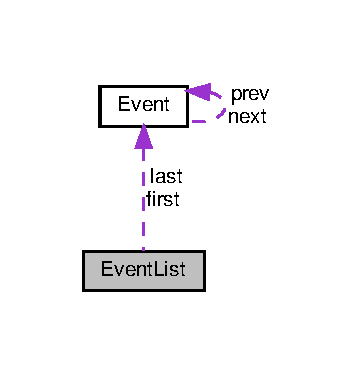
\includegraphics[width=170pt]{struct_event_list__coll__graph}
\end{center}
\end{figure}
\subsection*{Data Fields}
\begin{DoxyCompactItemize}
\item 
\hyperlink{struct_event}{Event} $\ast$ \hyperlink{struct_event_list_ab866d72c6e161e5eb85d4940b0dbc62e}{first}
\item 
\hyperlink{struct_event}{Event} $\ast$ \hyperlink{struct_event_list_a8e52f53a3606d45d86182ce606e9369d}{last}
\end{DoxyCompactItemize}


\subsection{Field Documentation}
\mbox{\Hypertarget{struct_event_list_ab866d72c6e161e5eb85d4940b0dbc62e}\label{struct_event_list_ab866d72c6e161e5eb85d4940b0dbc62e}} 
\index{Event\+List@{Event\+List}!first@{first}}
\index{first@{first}!Event\+List@{Event\+List}}
\subsubsection{\texorpdfstring{first}{first}}
{\footnotesize\ttfamily \hyperlink{struct_event}{Event}$\ast$ first}

\mbox{\Hypertarget{struct_event_list_a8e52f53a3606d45d86182ce606e9369d}\label{struct_event_list_a8e52f53a3606d45d86182ce606e9369d}} 
\index{Event\+List@{Event\+List}!last@{last}}
\index{last@{last}!Event\+List@{Event\+List}}
\subsubsection{\texorpdfstring{last}{last}}
{\footnotesize\ttfamily \hyperlink{struct_event}{Event}$\ast$ last}



The documentation for this struct was generated from the following file\+:\begin{DoxyCompactItemize}
\item 
/home/dani/\+Documents/egyetem/prog1/nagyhazi/hazi2/calendar2/calendar/\hyperlink{structures_8h}{structures.\+h}\end{DoxyCompactItemize}

\hypertarget{struct_find_list}{}\section{Find\+List Struct Reference}
\label{struct_find_list}\index{Find\+List@{Find\+List}}


{\ttfamily \#include $<$structures.\+h$>$}

\subsection*{Data Fields}
\begin{DoxyCompactItemize}
\item 
\hyperlink{struct_found_event}{Found\+Event} $\ast$ \hyperlink{struct_find_list_a9f9781ae49412999177095cb5e8c79d1}{first}
\item 
\hyperlink{struct_found_event}{Found\+Event} $\ast$ \hyperlink{struct_find_list_ab61e64643b8233c6d9feef3e2aaffef2}{last}
\end{DoxyCompactItemize}


\subsection{Detailed Description}
A keresés által talált események listája 

\subsection{Field Documentation}
\mbox{\Hypertarget{struct_find_list_a9f9781ae49412999177095cb5e8c79d1}\label{struct_find_list_a9f9781ae49412999177095cb5e8c79d1}} 
\index{Find\+List@{Find\+List}!first@{first}}
\index{first@{first}!Find\+List@{Find\+List}}
\subsubsection{\texorpdfstring{first}{first}}
{\footnotesize\ttfamily \hyperlink{struct_found_event}{Found\+Event}$\ast$ first}

a találati lista első őrszeme, üres \mbox{\Hypertarget{struct_find_list_ab61e64643b8233c6d9feef3e2aaffef2}\label{struct_find_list_ab61e64643b8233c6d9feef3e2aaffef2}} 
\index{Find\+List@{Find\+List}!last@{last}}
\index{last@{last}!Find\+List@{Find\+List}}
\subsubsection{\texorpdfstring{last}{last}}
{\footnotesize\ttfamily \hyperlink{struct_found_event}{Found\+Event}$\ast$ last}

a találati lista utolsó őrszeme, üres 

The documentation for this struct was generated from the following file\+:\begin{DoxyCompactItemize}
\item 
/home/dani/\+Documents/egyetem/prog1/nagyhazi/hazi2/calendar2/calendar/\hyperlink{structures_8h}{structures.\+h}\end{DoxyCompactItemize}

\hypertarget{struct_found_event}{}\section{Found\+Event Struct Reference}
\label{struct_found_event}\index{Found\+Event@{Found\+Event}}


{\ttfamily \#include $<$structures.\+h$>$}

\subsection*{Data Fields}
\begin{DoxyCompactItemize}
\item 
\hyperlink{struct_event}{Event} $\ast$ \hyperlink{struct_found_event_a9fb10dd8687d775ac50c8824bde19d67}{foundevent}
\item 
struct \hyperlink{struct_found_event}{Found\+Event} $\ast$ \hyperlink{struct_found_event_add29159b298db5eb8c68bd9314e7c498}{prevfound}
\item 
struct \hyperlink{struct_found_event}{Found\+Event} $\ast$ \hyperlink{struct_found_event_acbce65ffd090e8c5d45aa15b2ccdf453}{nextfound}
\end{DoxyCompactItemize}


\subsection{Field Documentation}
\mbox{\Hypertarget{struct_found_event_a9fb10dd8687d775ac50c8824bde19d67}\label{struct_found_event_a9fb10dd8687d775ac50c8824bde19d67}} 
\index{Found\+Event@{Found\+Event}!foundevent@{foundevent}}
\index{foundevent@{foundevent}!Found\+Event@{Found\+Event}}
\subsubsection{\texorpdfstring{foundevent}{foundevent}}
{\footnotesize\ttfamily \hyperlink{struct_event}{Event}$\ast$ foundevent}

\mbox{\Hypertarget{struct_found_event_acbce65ffd090e8c5d45aa15b2ccdf453}\label{struct_found_event_acbce65ffd090e8c5d45aa15b2ccdf453}} 
\index{Found\+Event@{Found\+Event}!nextfound@{nextfound}}
\index{nextfound@{nextfound}!Found\+Event@{Found\+Event}}
\subsubsection{\texorpdfstring{nextfound}{nextfound}}
{\footnotesize\ttfamily struct \hyperlink{struct_found_event}{Found\+Event}$\ast$ nextfound}

\mbox{\Hypertarget{struct_found_event_add29159b298db5eb8c68bd9314e7c498}\label{struct_found_event_add29159b298db5eb8c68bd9314e7c498}} 
\index{Found\+Event@{Found\+Event}!prevfound@{prevfound}}
\index{prevfound@{prevfound}!Found\+Event@{Found\+Event}}
\subsubsection{\texorpdfstring{prevfound}{prevfound}}
{\footnotesize\ttfamily struct \hyperlink{struct_found_event}{Found\+Event}$\ast$ prevfound}



The documentation for this struct was generated from the following file\+:\begin{DoxyCompactItemize}
\item 
/home/dani/\+Documents/egyetem/prog1/nagyhazi/hazi2/calendar2/calendar/\hyperlink{structures_8h}{structures.\+h}\end{DoxyCompactItemize}

\hypertarget{struct_lefoglalt}{}\section{Lefoglalt Struct Reference}
\label{struct_lefoglalt}\index{Lefoglalt@{Lefoglalt}}


Collaboration diagram for Lefoglalt\+:\nopagebreak
\begin{figure}[H]
\begin{center}
\leavevmode
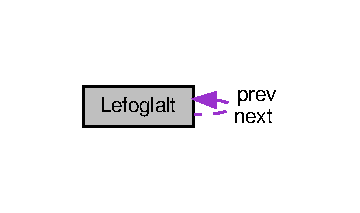
\includegraphics[width=173pt]{struct_lefoglalt__coll__graph}
\end{center}
\end{figure}
\subsection*{Data Fields}
\begin{DoxyCompactItemize}
\item 
void $\ast$ \hyperlink{struct_lefoglalt_a59522ad17870bd526fae5bbbc8125966}{valodi}
\item 
void $\ast$ \hyperlink{struct_lefoglalt_a58c09d4017310a90fad327e926330b96}{usernek}
\item 
size\+\_\+t \hyperlink{struct_lefoglalt_a7054394a4199245d774ead13d3bed5d6}{meret}
\item 
char \hyperlink{struct_lefoglalt_abfdd6d3e984090f35c264b15cf69c81a}{fv} \mbox{[}16\mbox{]}
\item 
char \hyperlink{struct_lefoglalt_aa8cbe4c2c142597b17ff65623129109f}{cel} \mbox{[}128\mbox{]}
\item 
char \hyperlink{struct_lefoglalt_a353d29f9f9cc0db6fca9d49b5f88d34d}{file} \mbox{[}64\mbox{]}
\item 
unsigned \hyperlink{struct_lefoglalt_a05ef0c4dbeec4fc8ccb225de9c26d896}{line}
\item 
struct \hyperlink{struct_lefoglalt}{Lefoglalt} $\ast$ \hyperlink{struct_lefoglalt_a2b1e290e1bec4c24cb7ec2aaf8747687}{prev}
\item 
struct \hyperlink{struct_lefoglalt}{Lefoglalt} $\ast$ \hyperlink{struct_lefoglalt_adc30abdfb5e692e2c216e3673d0d19b9}{next}
\end{DoxyCompactItemize}


\subsection{Field Documentation}
\mbox{\Hypertarget{struct_lefoglalt_aa8cbe4c2c142597b17ff65623129109f}\label{struct_lefoglalt_aa8cbe4c2c142597b17ff65623129109f}} 
\index{Lefoglalt@{Lefoglalt}!cel@{cel}}
\index{cel@{cel}!Lefoglalt@{Lefoglalt}}
\subsubsection{\texorpdfstring{cel}{cel}}
{\footnotesize\ttfamily char cel\mbox{[}128\mbox{]}}

\mbox{\Hypertarget{struct_lefoglalt_a353d29f9f9cc0db6fca9d49b5f88d34d}\label{struct_lefoglalt_a353d29f9f9cc0db6fca9d49b5f88d34d}} 
\index{Lefoglalt@{Lefoglalt}!file@{file}}
\index{file@{file}!Lefoglalt@{Lefoglalt}}
\subsubsection{\texorpdfstring{file}{file}}
{\footnotesize\ttfamily char file\mbox{[}64\mbox{]}}

\mbox{\Hypertarget{struct_lefoglalt_abfdd6d3e984090f35c264b15cf69c81a}\label{struct_lefoglalt_abfdd6d3e984090f35c264b15cf69c81a}} 
\index{Lefoglalt@{Lefoglalt}!fv@{fv}}
\index{fv@{fv}!Lefoglalt@{Lefoglalt}}
\subsubsection{\texorpdfstring{fv}{fv}}
{\footnotesize\ttfamily char fv\mbox{[}16\mbox{]}}

\mbox{\Hypertarget{struct_lefoglalt_a05ef0c4dbeec4fc8ccb225de9c26d896}\label{struct_lefoglalt_a05ef0c4dbeec4fc8ccb225de9c26d896}} 
\index{Lefoglalt@{Lefoglalt}!line@{line}}
\index{line@{line}!Lefoglalt@{Lefoglalt}}
\subsubsection{\texorpdfstring{line}{line}}
{\footnotesize\ttfamily unsigned line}

\mbox{\Hypertarget{struct_lefoglalt_a7054394a4199245d774ead13d3bed5d6}\label{struct_lefoglalt_a7054394a4199245d774ead13d3bed5d6}} 
\index{Lefoglalt@{Lefoglalt}!meret@{meret}}
\index{meret@{meret}!Lefoglalt@{Lefoglalt}}
\subsubsection{\texorpdfstring{meret}{meret}}
{\footnotesize\ttfamily size\+\_\+t meret}

\mbox{\Hypertarget{struct_lefoglalt_adc30abdfb5e692e2c216e3673d0d19b9}\label{struct_lefoglalt_adc30abdfb5e692e2c216e3673d0d19b9}} 
\index{Lefoglalt@{Lefoglalt}!next@{next}}
\index{next@{next}!Lefoglalt@{Lefoglalt}}
\subsubsection{\texorpdfstring{next}{next}}
{\footnotesize\ttfamily struct \hyperlink{struct_lefoglalt}{Lefoglalt} $\ast$ next}

\mbox{\Hypertarget{struct_lefoglalt_a2b1e290e1bec4c24cb7ec2aaf8747687}\label{struct_lefoglalt_a2b1e290e1bec4c24cb7ec2aaf8747687}} 
\index{Lefoglalt@{Lefoglalt}!prev@{prev}}
\index{prev@{prev}!Lefoglalt@{Lefoglalt}}
\subsubsection{\texorpdfstring{prev}{prev}}
{\footnotesize\ttfamily struct \hyperlink{struct_lefoglalt}{Lefoglalt}$\ast$ prev}

\mbox{\Hypertarget{struct_lefoglalt_a58c09d4017310a90fad327e926330b96}\label{struct_lefoglalt_a58c09d4017310a90fad327e926330b96}} 
\index{Lefoglalt@{Lefoglalt}!usernek@{usernek}}
\index{usernek@{usernek}!Lefoglalt@{Lefoglalt}}
\subsubsection{\texorpdfstring{usernek}{usernek}}
{\footnotesize\ttfamily void$\ast$ usernek}

\mbox{\Hypertarget{struct_lefoglalt_a59522ad17870bd526fae5bbbc8125966}\label{struct_lefoglalt_a59522ad17870bd526fae5bbbc8125966}} 
\index{Lefoglalt@{Lefoglalt}!valodi@{valodi}}
\index{valodi@{valodi}!Lefoglalt@{Lefoglalt}}
\subsubsection{\texorpdfstring{valodi}{valodi}}
{\footnotesize\ttfamily void$\ast$ valodi}



The documentation for this struct was generated from the following file\+:\begin{DoxyCompactItemize}
\item 
/home/dani/\+Documents/egyetem/prog1/nagyhazi/hazi2/calendar2/calendar/\hyperlink{debugmalloc_8c}{debugmalloc.\+c}\end{DoxyCompactItemize}

\hypertarget{struct_menu_pont}{}\section{Menu\+Pont Struct Reference}
\label{struct_menu_pont}\index{Menu\+Pont@{Menu\+Pont}}


{\ttfamily \#include $<$structures.\+h$>$}

\subsection*{Data Fields}
\begin{DoxyCompactItemize}
\item 
char const  $\ast$ \hyperlink{struct_menu_pont_a21c8b004e3b92cd18b29f8a51717956d}{nev}
\end{DoxyCompactItemize}


\subsection{Detailed Description}
Menupontok neveinek listája 

\subsection{Field Documentation}
\mbox{\Hypertarget{struct_menu_pont_a21c8b004e3b92cd18b29f8a51717956d}\label{struct_menu_pont_a21c8b004e3b92cd18b29f8a51717956d}} 
\index{Menu\+Pont@{Menu\+Pont}!nev@{nev}}
\index{nev@{nev}!Menu\+Pont@{Menu\+Pont}}
\subsubsection{\texorpdfstring{nev}{nev}}
{\footnotesize\ttfamily char const$\ast$ nev}

menüpont nevére mutató karaktertömb 

The documentation for this struct was generated from the following file\+:\begin{DoxyCompactItemize}
\item 
/home/dani/\+Documents/egyetem/prog1/nagyhazi/hazi2/calendar2/calendar/\hyperlink{structures_8h}{structures.\+h}\end{DoxyCompactItemize}

\hypertarget{struct_search_conditions}{}\section{Search\+Conditions Struct Reference}
\label{struct_search_conditions}\index{Search\+Conditions@{Search\+Conditions}}


{\ttfamily \#include $<$structures.\+h$>$}

\subsection*{Data Fields}
\begin{DoxyCompactItemize}
\item 
char $\ast$ \hyperlink{struct_search_conditions_a5ac083a645d964373f022d03df4849c8}{name}
\item 
int \hyperlink{struct_search_conditions_abeac221e38b7b9ce7df8722c842bf671}{year}
\item 
int \hyperlink{struct_search_conditions_a3560bdec25d509ef8f4f02409eaa9f1d}{week}
\item 
int \hyperlink{struct_search_conditions_aedb06abe5aff12fa3e7e0e71a374edfb}{month}
\item 
int \hyperlink{struct_search_conditions_a4c11afc03fc3ee49bab660def6558f2a}{day}
\end{DoxyCompactItemize}


\subsection{Field Documentation}
\mbox{\Hypertarget{struct_search_conditions_a4c11afc03fc3ee49bab660def6558f2a}\label{struct_search_conditions_a4c11afc03fc3ee49bab660def6558f2a}} 
\index{Search\+Conditions@{Search\+Conditions}!day@{day}}
\index{day@{day}!Search\+Conditions@{Search\+Conditions}}
\subsubsection{\texorpdfstring{day}{day}}
{\footnotesize\ttfamily int day}

\mbox{\Hypertarget{struct_search_conditions_aedb06abe5aff12fa3e7e0e71a374edfb}\label{struct_search_conditions_aedb06abe5aff12fa3e7e0e71a374edfb}} 
\index{Search\+Conditions@{Search\+Conditions}!month@{month}}
\index{month@{month}!Search\+Conditions@{Search\+Conditions}}
\subsubsection{\texorpdfstring{month}{month}}
{\footnotesize\ttfamily int month}

\mbox{\Hypertarget{struct_search_conditions_a5ac083a645d964373f022d03df4849c8}\label{struct_search_conditions_a5ac083a645d964373f022d03df4849c8}} 
\index{Search\+Conditions@{Search\+Conditions}!name@{name}}
\index{name@{name}!Search\+Conditions@{Search\+Conditions}}
\subsubsection{\texorpdfstring{name}{name}}
{\footnotesize\ttfamily char$\ast$ name}

\mbox{\Hypertarget{struct_search_conditions_a3560bdec25d509ef8f4f02409eaa9f1d}\label{struct_search_conditions_a3560bdec25d509ef8f4f02409eaa9f1d}} 
\index{Search\+Conditions@{Search\+Conditions}!week@{week}}
\index{week@{week}!Search\+Conditions@{Search\+Conditions}}
\subsubsection{\texorpdfstring{week}{week}}
{\footnotesize\ttfamily int week}

\mbox{\Hypertarget{struct_search_conditions_abeac221e38b7b9ce7df8722c842bf671}\label{struct_search_conditions_abeac221e38b7b9ce7df8722c842bf671}} 
\index{Search\+Conditions@{Search\+Conditions}!year@{year}}
\index{year@{year}!Search\+Conditions@{Search\+Conditions}}
\subsubsection{\texorpdfstring{year}{year}}
{\footnotesize\ttfamily int year}



The documentation for this struct was generated from the following file\+:\begin{DoxyCompactItemize}
\item 
/home/dani/\+Documents/egyetem/prog1/nagyhazi/hazi2/calendar2/calendar/\hyperlink{structures_8h}{structures.\+h}\end{DoxyCompactItemize}

\chapter{File Documentation}
\hypertarget{debugmalloc_8c}{}\section{/home/dani/\+Documents/egyetem/prog1/nagyhazi/hazi2/calendar2/calendar/debugmalloc.c File Reference}
\label{debugmalloc_8c}\index{/home/dani/\+Documents/egyetem/prog1/nagyhazi/hazi2/calendar2/calendar/debugmalloc.\+c@{/home/dani/\+Documents/egyetem/prog1/nagyhazi/hazi2/calendar2/calendar/debugmalloc.\+c}}
{\ttfamily \#include $<$stdbool.\+h$>$}\newline
{\ttfamily \#include $<$stdlib.\+h$>$}\newline
{\ttfamily \#include $<$stdio.\+h$>$}\newline
{\ttfamily \#include $<$ctype.\+h$>$}\newline
{\ttfamily \#include $<$string.\+h$>$}\newline
{\ttfamily \#include $<$time.\+h$>$}\newline
{\ttfamily \#include $<$stdarg.\+h$>$}\newline
{\ttfamily \#include \char`\"{}debugmalloc.\+h\char`\"{}}\newline
\subsection*{Data Structures}
\begin{DoxyCompactItemize}
\item 
struct \hyperlink{struct_lefoglalt}{Lefoglalt}
\end{DoxyCompactItemize}
\subsection*{Macros}
\begin{DoxyCompactItemize}
\item 
\#define \hyperlink{debugmalloc_8c_a5d5ca1decbb4ee3ccdeb6db6ba45ba41}{T\+A\+B\+L\+A\+\_\+\+O\+S\+Z\+L\+O\+P\+OK}~256
\end{DoxyCompactItemize}
\subsection*{Typedefs}
\begin{DoxyCompactItemize}
\item 
typedef struct \hyperlink{struct_lefoglalt}{Lefoglalt} \hyperlink{debugmalloc_8c_a9045711bae196a1aaff9a38a2c193d19}{Lefoglalt}
\end{DoxyCompactItemize}
\subsection*{Functions}
\begin{DoxyCompactItemize}
\item 
size\+\_\+t \hyperlink{debugmalloc_8c_a8c9ec70628a684e1d6e2781f10a9ce74}{debugmalloc\+\_\+hash} (void $\ast$mem)
\item 
void \hyperlink{debugmalloc_8c_a5a4971a7e15f7777b075985f0dc76624}{debugmalloc\+\_\+naplofajl} (char const $\ast$nev)
\item 
void \hyperlink{debugmalloc_8c_af4f3fa6b1dbe5a06127d3074fee25758}{debugmalloc\+\_\+dump} ()
\item 
void $\ast$ \hyperlink{debugmalloc_8c_ac93439c705b1780a2e0c0392f0fb29ac}{debugmalloc\+\_\+malloc\+\_\+full} (size\+\_\+t meret, char const $\ast$fv, char const $\ast$cel, char const $\ast$file, unsigned line, bool zero)
\item 
void \hyperlink{debugmalloc_8c_a37c186b2e2e471ef7f0a50f98046017e}{debugmalloc\+\_\+free\+\_\+full} (void $\ast$mem, char const $\ast$fv, char const $\ast$file, unsigned line)
\item 
void $\ast$ \hyperlink{debugmalloc_8c_ab7c0c062a428bb154778a9ca6eb40e04}{debugmalloc\+\_\+realloc\+\_\+full} (void $\ast$oldmem, size\+\_\+t newsize, char const $\ast$fv, char const $\ast$cel, char const $\ast$file, unsigned line)
\item 
void $\ast$ \hyperlink{debugmalloc_8c_a2114257904b92a949d3fcc0eda775aaf}{debugmalloc\+\_\+malloc} (size\+\_\+t meret)
\item 
void $\ast$ \hyperlink{debugmalloc_8c_ad88e4b22596045c845856b2e11ddbff9}{debugmalloc\+\_\+calloc} (size\+\_\+t nmemb, size\+\_\+t meret)
\item 
void \hyperlink{debugmalloc_8c_aaefe8f6631edc5b13d5801390295740c}{debugmalloc\+\_\+free} (void $\ast$mem)
\item 
void $\ast$ \hyperlink{debugmalloc_8c_a3aa69b6369a6dfbde0de6e391171ea94}{debugmalloc\+\_\+realloc} (void $\ast$oldmem, size\+\_\+t meret)
\end{DoxyCompactItemize}


\subsection{Macro Definition Documentation}
\mbox{\Hypertarget{debugmalloc_8c_a5d5ca1decbb4ee3ccdeb6db6ba45ba41}\label{debugmalloc_8c_a5d5ca1decbb4ee3ccdeb6db6ba45ba41}} 
\index{debugmalloc.\+c@{debugmalloc.\+c}!T\+A\+B\+L\+A\+\_\+\+O\+S\+Z\+L\+O\+P\+OK@{T\+A\+B\+L\+A\+\_\+\+O\+S\+Z\+L\+O\+P\+OK}}
\index{T\+A\+B\+L\+A\+\_\+\+O\+S\+Z\+L\+O\+P\+OK@{T\+A\+B\+L\+A\+\_\+\+O\+S\+Z\+L\+O\+P\+OK}!debugmalloc.\+c@{debugmalloc.\+c}}
\subsubsection{\texorpdfstring{T\+A\+B\+L\+A\+\_\+\+O\+S\+Z\+L\+O\+P\+OK}{TABLA\_OSZLOPOK}}
{\footnotesize\ttfamily \#define T\+A\+B\+L\+A\+\_\+\+O\+S\+Z\+L\+O\+P\+OK~256}



\subsection{Typedef Documentation}
\mbox{\Hypertarget{debugmalloc_8c_a9045711bae196a1aaff9a38a2c193d19}\label{debugmalloc_8c_a9045711bae196a1aaff9a38a2c193d19}} 
\index{debugmalloc.\+c@{debugmalloc.\+c}!Lefoglalt@{Lefoglalt}}
\index{Lefoglalt@{Lefoglalt}!debugmalloc.\+c@{debugmalloc.\+c}}
\subsubsection{\texorpdfstring{Lefoglalt}{Lefoglalt}}
{\footnotesize\ttfamily typedef struct \hyperlink{struct_lefoglalt}{Lefoglalt}  \hyperlink{struct_lefoglalt}{Lefoglalt}}



\subsection{Function Documentation}
\mbox{\Hypertarget{debugmalloc_8c_ad88e4b22596045c845856b2e11ddbff9}\label{debugmalloc_8c_ad88e4b22596045c845856b2e11ddbff9}} 
\index{debugmalloc.\+c@{debugmalloc.\+c}!debugmalloc\+\_\+calloc@{debugmalloc\+\_\+calloc}}
\index{debugmalloc\+\_\+calloc@{debugmalloc\+\_\+calloc}!debugmalloc.\+c@{debugmalloc.\+c}}
\subsubsection{\texorpdfstring{debugmalloc\+\_\+calloc()}{debugmalloc\_calloc()}}
{\footnotesize\ttfamily void$\ast$ debugmalloc\+\_\+calloc (\begin{DoxyParamCaption}\item[{size\+\_\+t}]{nmemb,  }\item[{size\+\_\+t}]{meret }\end{DoxyParamCaption})}

\mbox{\Hypertarget{debugmalloc_8c_af4f3fa6b1dbe5a06127d3074fee25758}\label{debugmalloc_8c_af4f3fa6b1dbe5a06127d3074fee25758}} 
\index{debugmalloc.\+c@{debugmalloc.\+c}!debugmalloc\+\_\+dump@{debugmalloc\+\_\+dump}}
\index{debugmalloc\+\_\+dump@{debugmalloc\+\_\+dump}!debugmalloc.\+c@{debugmalloc.\+c}}
\subsubsection{\texorpdfstring{debugmalloc\+\_\+dump()}{debugmalloc\_dump()}}
{\footnotesize\ttfamily void debugmalloc\+\_\+dump (\begin{DoxyParamCaption}{ }\end{DoxyParamCaption})}

\mbox{\Hypertarget{debugmalloc_8c_aaefe8f6631edc5b13d5801390295740c}\label{debugmalloc_8c_aaefe8f6631edc5b13d5801390295740c}} 
\index{debugmalloc.\+c@{debugmalloc.\+c}!debugmalloc\+\_\+free@{debugmalloc\+\_\+free}}
\index{debugmalloc\+\_\+free@{debugmalloc\+\_\+free}!debugmalloc.\+c@{debugmalloc.\+c}}
\subsubsection{\texorpdfstring{debugmalloc\+\_\+free()}{debugmalloc\_free()}}
{\footnotesize\ttfamily void debugmalloc\+\_\+free (\begin{DoxyParamCaption}\item[{void $\ast$}]{mem }\end{DoxyParamCaption})}

\mbox{\Hypertarget{debugmalloc_8c_a37c186b2e2e471ef7f0a50f98046017e}\label{debugmalloc_8c_a37c186b2e2e471ef7f0a50f98046017e}} 
\index{debugmalloc.\+c@{debugmalloc.\+c}!debugmalloc\+\_\+free\+\_\+full@{debugmalloc\+\_\+free\+\_\+full}}
\index{debugmalloc\+\_\+free\+\_\+full@{debugmalloc\+\_\+free\+\_\+full}!debugmalloc.\+c@{debugmalloc.\+c}}
\subsubsection{\texorpdfstring{debugmalloc\+\_\+free\+\_\+full()}{debugmalloc\_free\_full()}}
{\footnotesize\ttfamily void debugmalloc\+\_\+free\+\_\+full (\begin{DoxyParamCaption}\item[{void $\ast$}]{mem,  }\item[{char const $\ast$}]{fv,  }\item[{char const $\ast$}]{file,  }\item[{unsigned}]{line }\end{DoxyParamCaption})}

\mbox{\Hypertarget{debugmalloc_8c_a8c9ec70628a684e1d6e2781f10a9ce74}\label{debugmalloc_8c_a8c9ec70628a684e1d6e2781f10a9ce74}} 
\index{debugmalloc.\+c@{debugmalloc.\+c}!debugmalloc\+\_\+hash@{debugmalloc\+\_\+hash}}
\index{debugmalloc\+\_\+hash@{debugmalloc\+\_\+hash}!debugmalloc.\+c@{debugmalloc.\+c}}
\subsubsection{\texorpdfstring{debugmalloc\+\_\+hash()}{debugmalloc\_hash()}}
{\footnotesize\ttfamily size\+\_\+t debugmalloc\+\_\+hash (\begin{DoxyParamCaption}\item[{void $\ast$}]{mem }\end{DoxyParamCaption})}

\mbox{\Hypertarget{debugmalloc_8c_a2114257904b92a949d3fcc0eda775aaf}\label{debugmalloc_8c_a2114257904b92a949d3fcc0eda775aaf}} 
\index{debugmalloc.\+c@{debugmalloc.\+c}!debugmalloc\+\_\+malloc@{debugmalloc\+\_\+malloc}}
\index{debugmalloc\+\_\+malloc@{debugmalloc\+\_\+malloc}!debugmalloc.\+c@{debugmalloc.\+c}}
\subsubsection{\texorpdfstring{debugmalloc\+\_\+malloc()}{debugmalloc\_malloc()}}
{\footnotesize\ttfamily void$\ast$ debugmalloc\+\_\+malloc (\begin{DoxyParamCaption}\item[{size\+\_\+t}]{meret }\end{DoxyParamCaption})}

\mbox{\Hypertarget{debugmalloc_8c_ac93439c705b1780a2e0c0392f0fb29ac}\label{debugmalloc_8c_ac93439c705b1780a2e0c0392f0fb29ac}} 
\index{debugmalloc.\+c@{debugmalloc.\+c}!debugmalloc\+\_\+malloc\+\_\+full@{debugmalloc\+\_\+malloc\+\_\+full}}
\index{debugmalloc\+\_\+malloc\+\_\+full@{debugmalloc\+\_\+malloc\+\_\+full}!debugmalloc.\+c@{debugmalloc.\+c}}
\subsubsection{\texorpdfstring{debugmalloc\+\_\+malloc\+\_\+full()}{debugmalloc\_malloc\_full()}}
{\footnotesize\ttfamily void$\ast$ debugmalloc\+\_\+malloc\+\_\+full (\begin{DoxyParamCaption}\item[{size\+\_\+t}]{meret,  }\item[{char const $\ast$}]{fv,  }\item[{char const $\ast$}]{cel,  }\item[{char const $\ast$}]{file,  }\item[{unsigned}]{line,  }\item[{bool}]{zero }\end{DoxyParamCaption})}

\mbox{\Hypertarget{debugmalloc_8c_a5a4971a7e15f7777b075985f0dc76624}\label{debugmalloc_8c_a5a4971a7e15f7777b075985f0dc76624}} 
\index{debugmalloc.\+c@{debugmalloc.\+c}!debugmalloc\+\_\+naplofajl@{debugmalloc\+\_\+naplofajl}}
\index{debugmalloc\+\_\+naplofajl@{debugmalloc\+\_\+naplofajl}!debugmalloc.\+c@{debugmalloc.\+c}}
\subsubsection{\texorpdfstring{debugmalloc\+\_\+naplofajl()}{debugmalloc\_naplofajl()}}
{\footnotesize\ttfamily void debugmalloc\+\_\+naplofajl (\begin{DoxyParamCaption}\item[{char const $\ast$}]{nev }\end{DoxyParamCaption})}

\mbox{\Hypertarget{debugmalloc_8c_a3aa69b6369a6dfbde0de6e391171ea94}\label{debugmalloc_8c_a3aa69b6369a6dfbde0de6e391171ea94}} 
\index{debugmalloc.\+c@{debugmalloc.\+c}!debugmalloc\+\_\+realloc@{debugmalloc\+\_\+realloc}}
\index{debugmalloc\+\_\+realloc@{debugmalloc\+\_\+realloc}!debugmalloc.\+c@{debugmalloc.\+c}}
\subsubsection{\texorpdfstring{debugmalloc\+\_\+realloc()}{debugmalloc\_realloc()}}
{\footnotesize\ttfamily void$\ast$ debugmalloc\+\_\+realloc (\begin{DoxyParamCaption}\item[{void $\ast$}]{oldmem,  }\item[{size\+\_\+t}]{meret }\end{DoxyParamCaption})}

\mbox{\Hypertarget{debugmalloc_8c_ab7c0c062a428bb154778a9ca6eb40e04}\label{debugmalloc_8c_ab7c0c062a428bb154778a9ca6eb40e04}} 
\index{debugmalloc.\+c@{debugmalloc.\+c}!debugmalloc\+\_\+realloc\+\_\+full@{debugmalloc\+\_\+realloc\+\_\+full}}
\index{debugmalloc\+\_\+realloc\+\_\+full@{debugmalloc\+\_\+realloc\+\_\+full}!debugmalloc.\+c@{debugmalloc.\+c}}
\subsubsection{\texorpdfstring{debugmalloc\+\_\+realloc\+\_\+full()}{debugmalloc\_realloc\_full()}}
{\footnotesize\ttfamily void$\ast$ debugmalloc\+\_\+realloc\+\_\+full (\begin{DoxyParamCaption}\item[{void $\ast$}]{oldmem,  }\item[{size\+\_\+t}]{newsize,  }\item[{char const $\ast$}]{fv,  }\item[{char const $\ast$}]{cel,  }\item[{char const $\ast$}]{file,  }\item[{unsigned}]{line }\end{DoxyParamCaption})}


\hypertarget{debugmalloc_8h}{}\section{/home/dani/\+Documents/egyetem/prog1/nagyhazi/hazi2/calendar2/calendar/debugmalloc.h File Reference}
\label{debugmalloc_8h}\index{/home/dani/\+Documents/egyetem/prog1/nagyhazi/hazi2/calendar2/calendar/debugmalloc.\+h@{/home/dani/\+Documents/egyetem/prog1/nagyhazi/hazi2/calendar2/calendar/debugmalloc.\+h}}
{\ttfamily \#include $<$stdlib.\+h$>$}\newline
{\ttfamily \#include $<$stdbool.\+h$>$}\newline
Include dependency graph for debugmalloc.\+h\+:\nopagebreak
\begin{figure}[H]
\begin{center}
\leavevmode
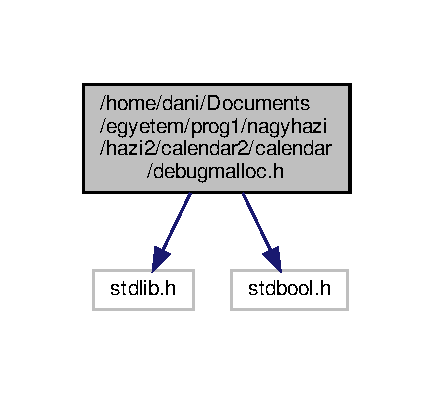
\includegraphics[width=208pt]{debugmalloc_8h__incl}
\end{center}
\end{figure}
This graph shows which files directly or indirectly include this file\+:\nopagebreak
\begin{figure}[H]
\begin{center}
\leavevmode
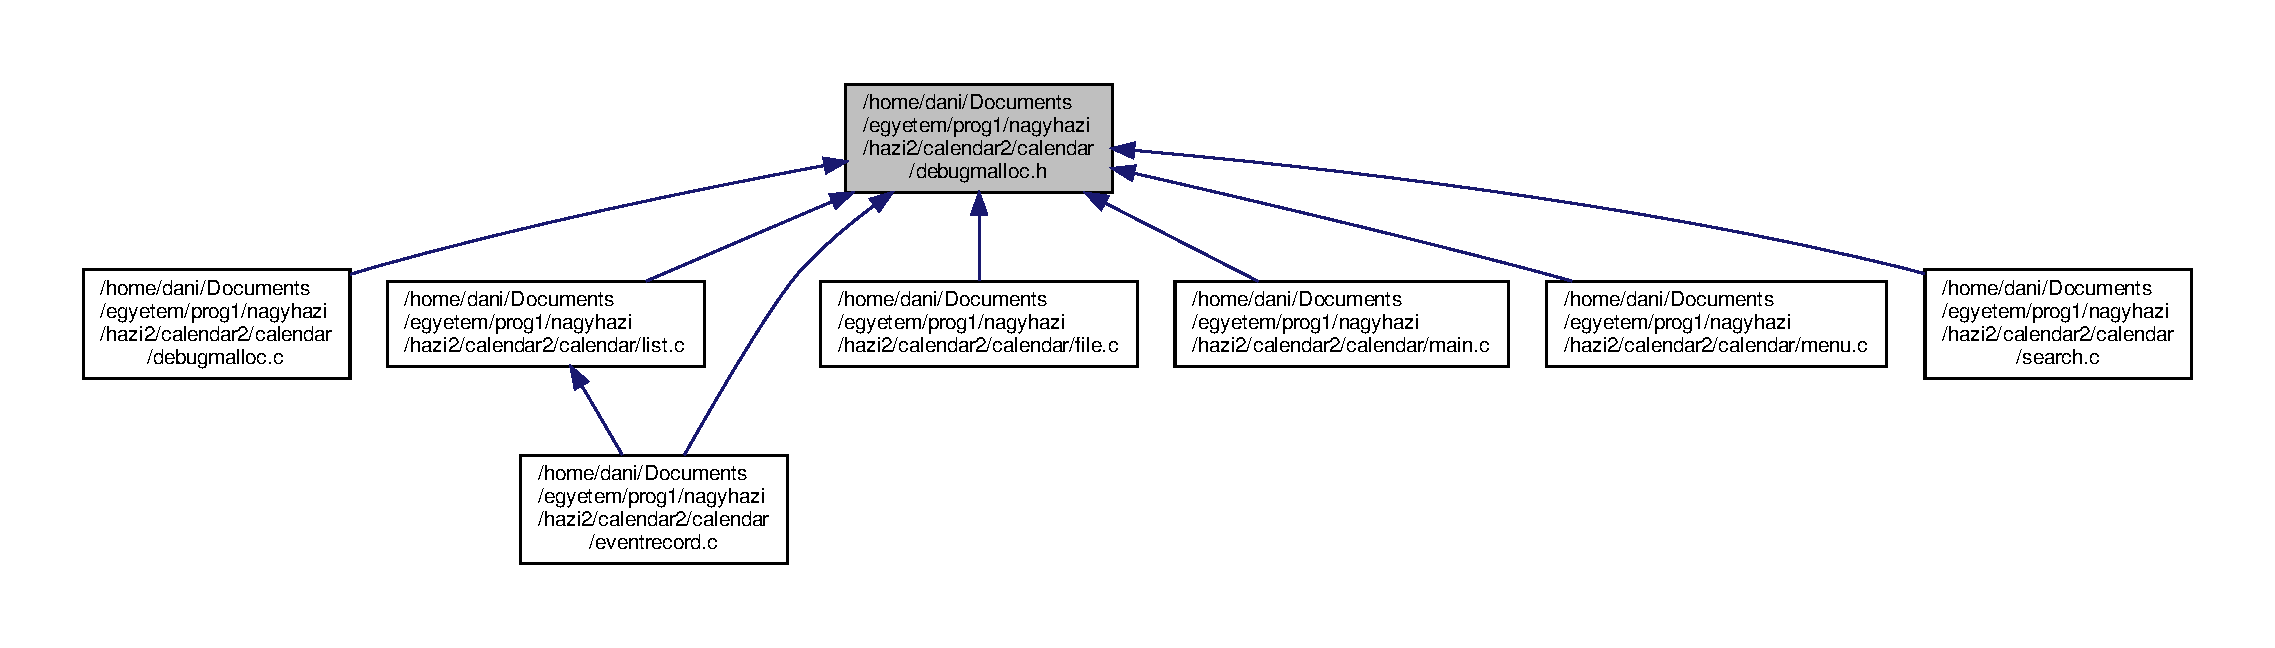
\includegraphics[width=350pt]{debugmalloc_8h__dep__incl}
\end{center}
\end{figure}
\subsection*{Macros}
\begin{DoxyCompactItemize}
\item 
\#define \hyperlink{debugmalloc_8h_a183c59bc3a5f5116f8490a9335db33a3}{malloc}(X)~\hyperlink{debugmalloc_8h_ac93439c705b1780a2e0c0392f0fb29ac}{debugmalloc\+\_\+malloc\+\_\+full}(X, \char`\"{}malloc\char`\"{}, \#X, \+\_\+\+\_\+\+F\+I\+L\+E\+\_\+\+\_\+, \+\_\+\+\_\+\+L\+I\+N\+E\+\_\+\+\_\+, false)
\item 
\#define \hyperlink{debugmalloc_8h_a1df39f6160f230fb8ed801481dbde0c0}{calloc}(X,  Y)~\hyperlink{debugmalloc_8h_ac93439c705b1780a2e0c0392f0fb29ac}{debugmalloc\+\_\+malloc\+\_\+full}(X$\ast$Y, \char`\"{}calloc\char`\"{}, \#X \char`\"{}, \char`\"{} \#Y, \+\_\+\+\_\+\+F\+I\+L\+E\+\_\+\+\_\+, \+\_\+\+\_\+\+L\+I\+N\+E\+\_\+\+\_\+, true)
\item 
\#define \hyperlink{debugmalloc_8h_adcb4d5ff54f988a9e07d7640e0b333e5}{realloc}(P,  X)~\hyperlink{debugmalloc_8h_a4668760068bcb278408fe4299c91ed42}{debugmalloc\+\_\+realloc\+\_\+full}(P, X, \char`\"{}realloc\char`\"{}, \#X, \+\_\+\+\_\+\+F\+I\+L\+E\+\_\+\+\_\+, \+\_\+\+\_\+\+L\+I\+N\+E\+\_\+\+\_\+)
\item 
\#define \hyperlink{debugmalloc_8h_aa7943e5d135734f6801bebcc37401fc0}{free}(P)~\hyperlink{debugmalloc_8h_a37c186b2e2e471ef7f0a50f98046017e}{debugmalloc\+\_\+free\+\_\+full}(P, \char`\"{}free\char`\"{}, \+\_\+\+\_\+\+F\+I\+L\+E\+\_\+\+\_\+, \+\_\+\+\_\+\+L\+I\+N\+E\+\_\+\+\_\+)
\end{DoxyCompactItemize}
\subsection*{Functions}
\begin{DoxyCompactItemize}
\item 
void \hyperlink{debugmalloc_8h_a5a4971a7e15f7777b075985f0dc76624}{debugmalloc\+\_\+naplofajl} (char const $\ast$nev)
\item 
void \hyperlink{debugmalloc_8h_af4f3fa6b1dbe5a06127d3074fee25758}{debugmalloc\+\_\+dump} ()
\item 
void $\ast$ \hyperlink{debugmalloc_8h_ac93439c705b1780a2e0c0392f0fb29ac}{debugmalloc\+\_\+malloc\+\_\+full} (size\+\_\+t meret, char const $\ast$fv, char const $\ast$cel, char const $\ast$file, unsigned line, bool zero)
\item 
void $\ast$ \hyperlink{debugmalloc_8h_a4668760068bcb278408fe4299c91ed42}{debugmalloc\+\_\+realloc\+\_\+full} (void $\ast$regimem, size\+\_\+t newsize, char const $\ast$fv, char const $\ast$cel, char const $\ast$file, unsigned line)
\item 
void \hyperlink{debugmalloc_8h_a37c186b2e2e471ef7f0a50f98046017e}{debugmalloc\+\_\+free\+\_\+full} (void $\ast$mem, char const $\ast$fv, char const $\ast$file, unsigned line)
\item 
void $\ast$ \hyperlink{debugmalloc_8h_a2114257904b92a949d3fcc0eda775aaf}{debugmalloc\+\_\+malloc} (size\+\_\+t meret)
\item 
void $\ast$ \hyperlink{debugmalloc_8h_ad88e4b22596045c845856b2e11ddbff9}{debugmalloc\+\_\+calloc} (size\+\_\+t nmemb, size\+\_\+t meret)
\item 
void $\ast$ \hyperlink{debugmalloc_8h_aae4fb167c406177989b98c73cb95e130}{debugmalloc\+\_\+realloc} (void $\ast$regimem, size\+\_\+t meret)
\item 
void \hyperlink{debugmalloc_8h_aaefe8f6631edc5b13d5801390295740c}{debugmalloc\+\_\+free} (void $\ast$mem)
\end{DoxyCompactItemize}


\subsection{Macro Definition Documentation}
\mbox{\Hypertarget{debugmalloc_8h_a1df39f6160f230fb8ed801481dbde0c0}\label{debugmalloc_8h_a1df39f6160f230fb8ed801481dbde0c0}} 
\index{debugmalloc.\+h@{debugmalloc.\+h}!calloc@{calloc}}
\index{calloc@{calloc}!debugmalloc.\+h@{debugmalloc.\+h}}
\subsubsection{\texorpdfstring{calloc}{calloc}}
{\footnotesize\ttfamily \#define calloc(\begin{DoxyParamCaption}\item[{}]{X,  }\item[{}]{Y }\end{DoxyParamCaption})~\hyperlink{debugmalloc_8h_ac93439c705b1780a2e0c0392f0fb29ac}{debugmalloc\+\_\+malloc\+\_\+full}(X$\ast$Y, \char`\"{}calloc\char`\"{}, \#X \char`\"{}, \char`\"{} \#Y, \+\_\+\+\_\+\+F\+I\+L\+E\+\_\+\+\_\+, \+\_\+\+\_\+\+L\+I\+N\+E\+\_\+\+\_\+, true)}

\mbox{\Hypertarget{debugmalloc_8h_aa7943e5d135734f6801bebcc37401fc0}\label{debugmalloc_8h_aa7943e5d135734f6801bebcc37401fc0}} 
\index{debugmalloc.\+h@{debugmalloc.\+h}!free@{free}}
\index{free@{free}!debugmalloc.\+h@{debugmalloc.\+h}}
\subsubsection{\texorpdfstring{free}{free}}
{\footnotesize\ttfamily \#define free(\begin{DoxyParamCaption}\item[{}]{P }\end{DoxyParamCaption})~\hyperlink{debugmalloc_8h_a37c186b2e2e471ef7f0a50f98046017e}{debugmalloc\+\_\+free\+\_\+full}(P, \char`\"{}free\char`\"{}, \+\_\+\+\_\+\+F\+I\+L\+E\+\_\+\+\_\+, \+\_\+\+\_\+\+L\+I\+N\+E\+\_\+\+\_\+)}

\mbox{\Hypertarget{debugmalloc_8h_a183c59bc3a5f5116f8490a9335db33a3}\label{debugmalloc_8h_a183c59bc3a5f5116f8490a9335db33a3}} 
\index{debugmalloc.\+h@{debugmalloc.\+h}!malloc@{malloc}}
\index{malloc@{malloc}!debugmalloc.\+h@{debugmalloc.\+h}}
\subsubsection{\texorpdfstring{malloc}{malloc}}
{\footnotesize\ttfamily \#define malloc(\begin{DoxyParamCaption}\item[{}]{X }\end{DoxyParamCaption})~\hyperlink{debugmalloc_8h_ac93439c705b1780a2e0c0392f0fb29ac}{debugmalloc\+\_\+malloc\+\_\+full}(X, \char`\"{}malloc\char`\"{}, \#X, \+\_\+\+\_\+\+F\+I\+L\+E\+\_\+\+\_\+, \+\_\+\+\_\+\+L\+I\+N\+E\+\_\+\+\_\+, false)}

\mbox{\Hypertarget{debugmalloc_8h_adcb4d5ff54f988a9e07d7640e0b333e5}\label{debugmalloc_8h_adcb4d5ff54f988a9e07d7640e0b333e5}} 
\index{debugmalloc.\+h@{debugmalloc.\+h}!realloc@{realloc}}
\index{realloc@{realloc}!debugmalloc.\+h@{debugmalloc.\+h}}
\subsubsection{\texorpdfstring{realloc}{realloc}}
{\footnotesize\ttfamily \#define realloc(\begin{DoxyParamCaption}\item[{}]{P,  }\item[{}]{X }\end{DoxyParamCaption})~\hyperlink{debugmalloc_8h_a4668760068bcb278408fe4299c91ed42}{debugmalloc\+\_\+realloc\+\_\+full}(P, X, \char`\"{}realloc\char`\"{}, \#X, \+\_\+\+\_\+\+F\+I\+L\+E\+\_\+\+\_\+, \+\_\+\+\_\+\+L\+I\+N\+E\+\_\+\+\_\+)}



\subsection{Function Documentation}
\mbox{\Hypertarget{debugmalloc_8h_ad88e4b22596045c845856b2e11ddbff9}\label{debugmalloc_8h_ad88e4b22596045c845856b2e11ddbff9}} 
\index{debugmalloc.\+h@{debugmalloc.\+h}!debugmalloc\+\_\+calloc@{debugmalloc\+\_\+calloc}}
\index{debugmalloc\+\_\+calloc@{debugmalloc\+\_\+calloc}!debugmalloc.\+h@{debugmalloc.\+h}}
\subsubsection{\texorpdfstring{debugmalloc\+\_\+calloc()}{debugmalloc\_calloc()}}
{\footnotesize\ttfamily void$\ast$ debugmalloc\+\_\+calloc (\begin{DoxyParamCaption}\item[{size\+\_\+t}]{nmemb,  }\item[{size\+\_\+t}]{meret }\end{DoxyParamCaption})}

Here is the call graph for this function\+:\nopagebreak
\begin{figure}[H]
\begin{center}
\leavevmode
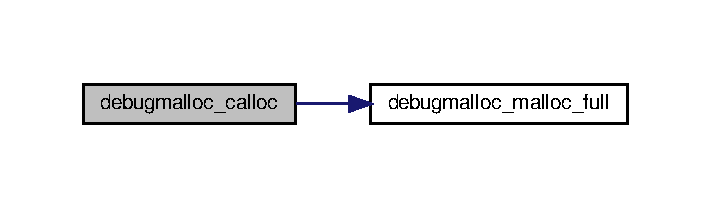
\includegraphics[width=341pt]{debugmalloc_8h_ad88e4b22596045c845856b2e11ddbff9_cgraph}
\end{center}
\end{figure}
\mbox{\Hypertarget{debugmalloc_8h_af4f3fa6b1dbe5a06127d3074fee25758}\label{debugmalloc_8h_af4f3fa6b1dbe5a06127d3074fee25758}} 
\index{debugmalloc.\+h@{debugmalloc.\+h}!debugmalloc\+\_\+dump@{debugmalloc\+\_\+dump}}
\index{debugmalloc\+\_\+dump@{debugmalloc\+\_\+dump}!debugmalloc.\+h@{debugmalloc.\+h}}
\subsubsection{\texorpdfstring{debugmalloc\+\_\+dump()}{debugmalloc\_dump()}}
{\footnotesize\ttfamily void debugmalloc\+\_\+dump (\begin{DoxyParamCaption}{ }\end{DoxyParamCaption})}

\mbox{\Hypertarget{debugmalloc_8h_aaefe8f6631edc5b13d5801390295740c}\label{debugmalloc_8h_aaefe8f6631edc5b13d5801390295740c}} 
\index{debugmalloc.\+h@{debugmalloc.\+h}!debugmalloc\+\_\+free@{debugmalloc\+\_\+free}}
\index{debugmalloc\+\_\+free@{debugmalloc\+\_\+free}!debugmalloc.\+h@{debugmalloc.\+h}}
\subsubsection{\texorpdfstring{debugmalloc\+\_\+free()}{debugmalloc\_free()}}
{\footnotesize\ttfamily void debugmalloc\+\_\+free (\begin{DoxyParamCaption}\item[{void $\ast$}]{mem }\end{DoxyParamCaption})}

Here is the call graph for this function\+:\nopagebreak
\begin{figure}[H]
\begin{center}
\leavevmode
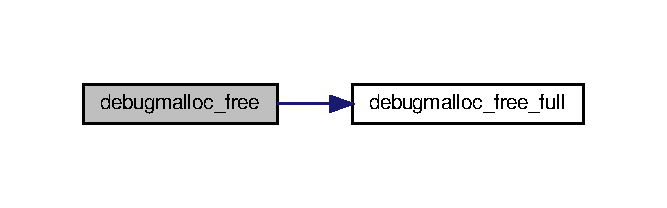
\includegraphics[width=320pt]{debugmalloc_8h_aaefe8f6631edc5b13d5801390295740c_cgraph}
\end{center}
\end{figure}
\mbox{\Hypertarget{debugmalloc_8h_a37c186b2e2e471ef7f0a50f98046017e}\label{debugmalloc_8h_a37c186b2e2e471ef7f0a50f98046017e}} 
\index{debugmalloc.\+h@{debugmalloc.\+h}!debugmalloc\+\_\+free\+\_\+full@{debugmalloc\+\_\+free\+\_\+full}}
\index{debugmalloc\+\_\+free\+\_\+full@{debugmalloc\+\_\+free\+\_\+full}!debugmalloc.\+h@{debugmalloc.\+h}}
\subsubsection{\texorpdfstring{debugmalloc\+\_\+free\+\_\+full()}{debugmalloc\_free\_full()}}
{\footnotesize\ttfamily void debugmalloc\+\_\+free\+\_\+full (\begin{DoxyParamCaption}\item[{void $\ast$}]{mem,  }\item[{char const $\ast$}]{fv,  }\item[{char const $\ast$}]{file,  }\item[{unsigned}]{line }\end{DoxyParamCaption})}

Here is the caller graph for this function\+:\nopagebreak
\begin{figure}[H]
\begin{center}
\leavevmode
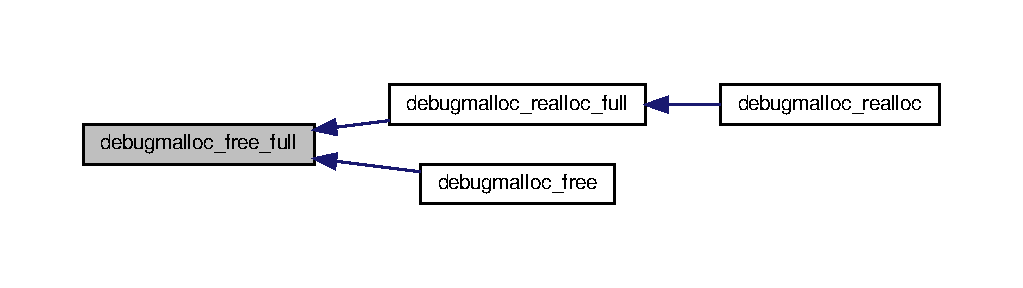
\includegraphics[width=350pt]{debugmalloc_8h_a37c186b2e2e471ef7f0a50f98046017e_icgraph}
\end{center}
\end{figure}
\mbox{\Hypertarget{debugmalloc_8h_a2114257904b92a949d3fcc0eda775aaf}\label{debugmalloc_8h_a2114257904b92a949d3fcc0eda775aaf}} 
\index{debugmalloc.\+h@{debugmalloc.\+h}!debugmalloc\+\_\+malloc@{debugmalloc\+\_\+malloc}}
\index{debugmalloc\+\_\+malloc@{debugmalloc\+\_\+malloc}!debugmalloc.\+h@{debugmalloc.\+h}}
\subsubsection{\texorpdfstring{debugmalloc\+\_\+malloc()}{debugmalloc\_malloc()}}
{\footnotesize\ttfamily void$\ast$ debugmalloc\+\_\+malloc (\begin{DoxyParamCaption}\item[{size\+\_\+t}]{meret }\end{DoxyParamCaption})}

Here is the call graph for this function\+:\nopagebreak
\begin{figure}[H]
\begin{center}
\leavevmode
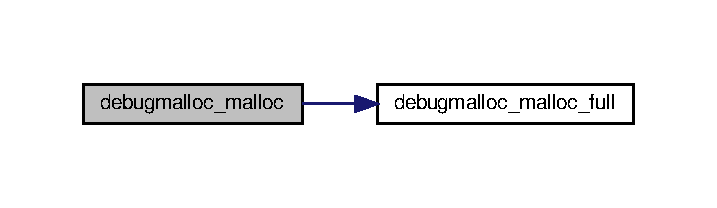
\includegraphics[width=344pt]{debugmalloc_8h_a2114257904b92a949d3fcc0eda775aaf_cgraph}
\end{center}
\end{figure}
\mbox{\Hypertarget{debugmalloc_8h_ac93439c705b1780a2e0c0392f0fb29ac}\label{debugmalloc_8h_ac93439c705b1780a2e0c0392f0fb29ac}} 
\index{debugmalloc.\+h@{debugmalloc.\+h}!debugmalloc\+\_\+malloc\+\_\+full@{debugmalloc\+\_\+malloc\+\_\+full}}
\index{debugmalloc\+\_\+malloc\+\_\+full@{debugmalloc\+\_\+malloc\+\_\+full}!debugmalloc.\+h@{debugmalloc.\+h}}
\subsubsection{\texorpdfstring{debugmalloc\+\_\+malloc\+\_\+full()}{debugmalloc\_malloc\_full()}}
{\footnotesize\ttfamily void$\ast$ debugmalloc\+\_\+malloc\+\_\+full (\begin{DoxyParamCaption}\item[{size\+\_\+t}]{meret,  }\item[{char const $\ast$}]{fv,  }\item[{char const $\ast$}]{cel,  }\item[{char const $\ast$}]{file,  }\item[{unsigned}]{line,  }\item[{bool}]{zero }\end{DoxyParamCaption})}

Here is the caller graph for this function\+:\nopagebreak
\begin{figure}[H]
\begin{center}
\leavevmode
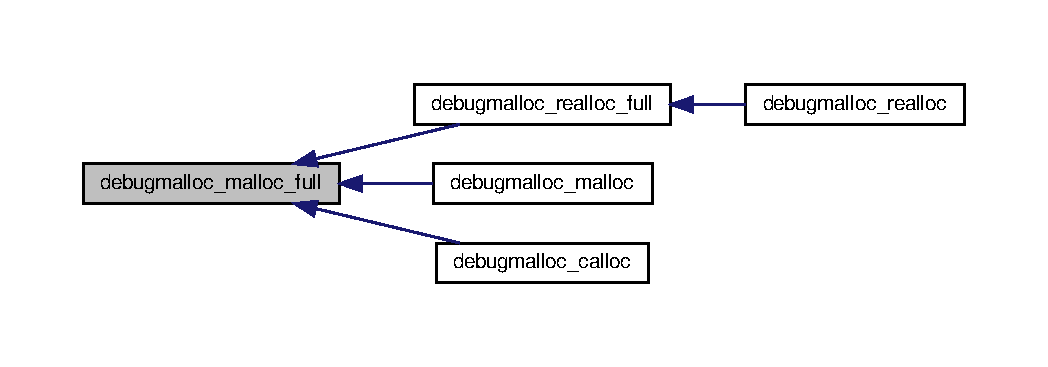
\includegraphics[width=350pt]{debugmalloc_8h_ac93439c705b1780a2e0c0392f0fb29ac_icgraph}
\end{center}
\end{figure}
\mbox{\Hypertarget{debugmalloc_8h_a5a4971a7e15f7777b075985f0dc76624}\label{debugmalloc_8h_a5a4971a7e15f7777b075985f0dc76624}} 
\index{debugmalloc.\+h@{debugmalloc.\+h}!debugmalloc\+\_\+naplofajl@{debugmalloc\+\_\+naplofajl}}
\index{debugmalloc\+\_\+naplofajl@{debugmalloc\+\_\+naplofajl}!debugmalloc.\+h@{debugmalloc.\+h}}
\subsubsection{\texorpdfstring{debugmalloc\+\_\+naplofajl()}{debugmalloc\_naplofajl()}}
{\footnotesize\ttfamily void debugmalloc\+\_\+naplofajl (\begin{DoxyParamCaption}\item[{char const $\ast$}]{nev }\end{DoxyParamCaption})}

\mbox{\Hypertarget{debugmalloc_8h_aae4fb167c406177989b98c73cb95e130}\label{debugmalloc_8h_aae4fb167c406177989b98c73cb95e130}} 
\index{debugmalloc.\+h@{debugmalloc.\+h}!debugmalloc\+\_\+realloc@{debugmalloc\+\_\+realloc}}
\index{debugmalloc\+\_\+realloc@{debugmalloc\+\_\+realloc}!debugmalloc.\+h@{debugmalloc.\+h}}
\subsubsection{\texorpdfstring{debugmalloc\+\_\+realloc()}{debugmalloc\_realloc()}}
{\footnotesize\ttfamily void$\ast$ debugmalloc\+\_\+realloc (\begin{DoxyParamCaption}\item[{void $\ast$}]{regimem,  }\item[{size\+\_\+t}]{meret }\end{DoxyParamCaption})}

Here is the call graph for this function\+:\nopagebreak
\begin{figure}[H]
\begin{center}
\leavevmode
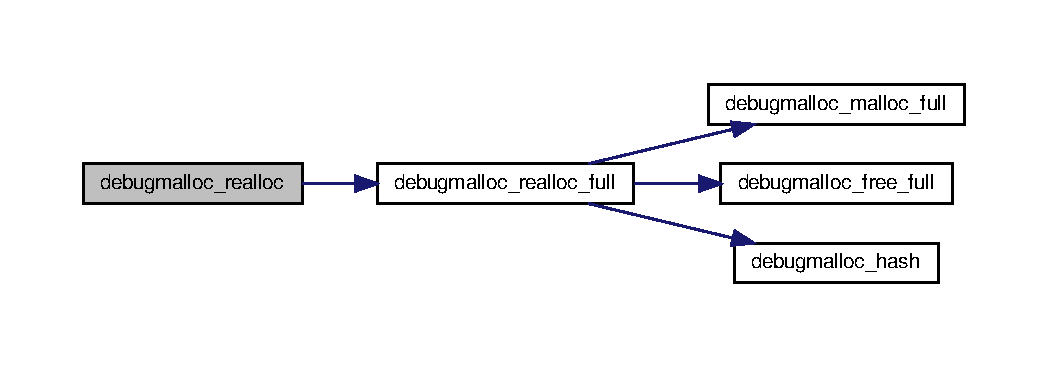
\includegraphics[width=350pt]{debugmalloc_8h_aae4fb167c406177989b98c73cb95e130_cgraph}
\end{center}
\end{figure}
\mbox{\Hypertarget{debugmalloc_8h_a4668760068bcb278408fe4299c91ed42}\label{debugmalloc_8h_a4668760068bcb278408fe4299c91ed42}} 
\index{debugmalloc.\+h@{debugmalloc.\+h}!debugmalloc\+\_\+realloc\+\_\+full@{debugmalloc\+\_\+realloc\+\_\+full}}
\index{debugmalloc\+\_\+realloc\+\_\+full@{debugmalloc\+\_\+realloc\+\_\+full}!debugmalloc.\+h@{debugmalloc.\+h}}
\subsubsection{\texorpdfstring{debugmalloc\+\_\+realloc\+\_\+full()}{debugmalloc\_realloc\_full()}}
{\footnotesize\ttfamily void$\ast$ debugmalloc\+\_\+realloc\+\_\+full (\begin{DoxyParamCaption}\item[{void $\ast$}]{regimem,  }\item[{size\+\_\+t}]{newsize,  }\item[{char const $\ast$}]{fv,  }\item[{char const $\ast$}]{cel,  }\item[{char const $\ast$}]{file,  }\item[{unsigned}]{line }\end{DoxyParamCaption})}

Here is the call graph for this function\+:\nopagebreak
\begin{figure}[H]
\begin{center}
\leavevmode
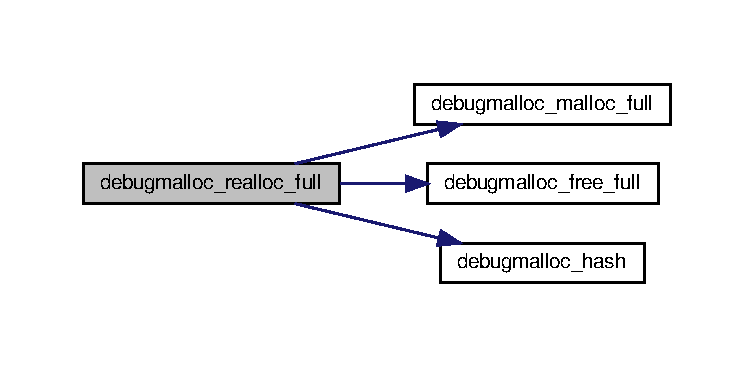
\includegraphics[width=350pt]{debugmalloc_8h_a4668760068bcb278408fe4299c91ed42_cgraph}
\end{center}
\end{figure}
Here is the caller graph for this function\+:\nopagebreak
\begin{figure}[H]
\begin{center}
\leavevmode
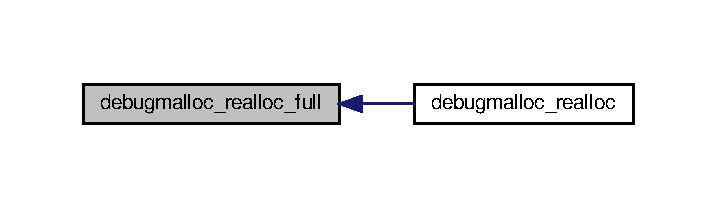
\includegraphics[width=344pt]{debugmalloc_8h_a4668760068bcb278408fe4299c91ed42_icgraph}
\end{center}
\end{figure}

\hypertarget{eventrecord_8c}{}\section{/home/dani/\+Documents/egyetem/prog1/nagyhazi/hazi2/calendar2/calendar/eventrecord.c File Reference}
\label{eventrecord_8c}\index{/home/dani/\+Documents/egyetem/prog1/nagyhazi/hazi2/calendar2/calendar/eventrecord.\+c@{/home/dani/\+Documents/egyetem/prog1/nagyhazi/hazi2/calendar2/calendar/eventrecord.\+c}}
{\ttfamily \#include \char`\"{}eventrecord.\+h\char`\"{}}\newline
{\ttfamily \#include \char`\"{}structures.\+h\char`\"{}}\newline
{\ttfamily \#include $<$stdio.\+h$>$}\newline
{\ttfamily \#include $<$stdbool.\+h$>$}\newline
{\ttfamily \#include \char`\"{}menu.\+h\char`\"{}}\newline
{\ttfamily \#include \char`\"{}list.\+h\char`\"{}}\newline
{\ttfamily \#include $<$stdlib.\+h$>$}\newline
\subsection*{Functions}
\begin{DoxyCompactItemize}
\item 
void \hyperlink{group__eventrecord_ga610dc34a1e251a16311ca7ac15f64e05}{moveevent} (\hyperlink{struct_event}{Event} $\ast$event, \hyperlink{struct_event_list}{Event\+List} const $\ast$eventlist, \hyperlink{group__eventrecord_ga643f8b09cbc45afc4ad36b27c077b1fd}{Mod\+By} modby)
\item 
void \hyperlink{group__eventrecord_gaf69a5ee77b139263897d5e6bfe7d7f2a}{deleteevent} (\hyperlink{struct_event}{Event} $\ast$event)
\item 
int \hyperlink{group__eventrecord_gac6e06e3186496cd8eb6618baf3ca9d3e}{scanrecordcommand} (bool isnewevent, int i, \hyperlink{struct_event}{Event} $\ast$event, \hyperlink{struct_event_list}{Event\+List} const $\ast$eventlist)
\item 
int \hyperlink{group__eventrecord_ga43a7dc247171d596d8d808776d8d40f5}{printeventrecord} (\hyperlink{struct_event}{Event} $\ast$event, \hyperlink{struct_search_conditions}{Search\+Conditions} condition, \hyperlink{struct_event_list}{Event\+List} $\ast$eventlist)
\end{DoxyCompactItemize}

\hypertarget{eventrecord_8h}{}\section{/home/dani/\+Documents/egyetem/prog1/nagyhazi/hazi2/calendar2/calendar/eventrecord.h File Reference}
\label{eventrecord_8h}\index{/home/dani/\+Documents/egyetem/prog1/nagyhazi/hazi2/calendar2/calendar/eventrecord.\+h@{/home/dani/\+Documents/egyetem/prog1/nagyhazi/hazi2/calendar2/calendar/eventrecord.\+h}}
{\ttfamily \#include \char`\"{}structures.\+h\char`\"{}}\newline
Include dependency graph for eventrecord.\+h\+:\nopagebreak
\begin{figure}[H]
\begin{center}
\leavevmode
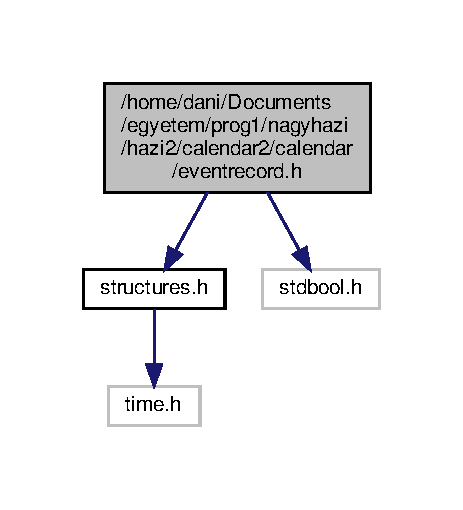
\includegraphics[width=208pt]{eventrecord_8h__incl}
\end{center}
\end{figure}
This graph shows which files directly or indirectly include this file\+:
\nopagebreak
\begin{figure}[H]
\begin{center}
\leavevmode
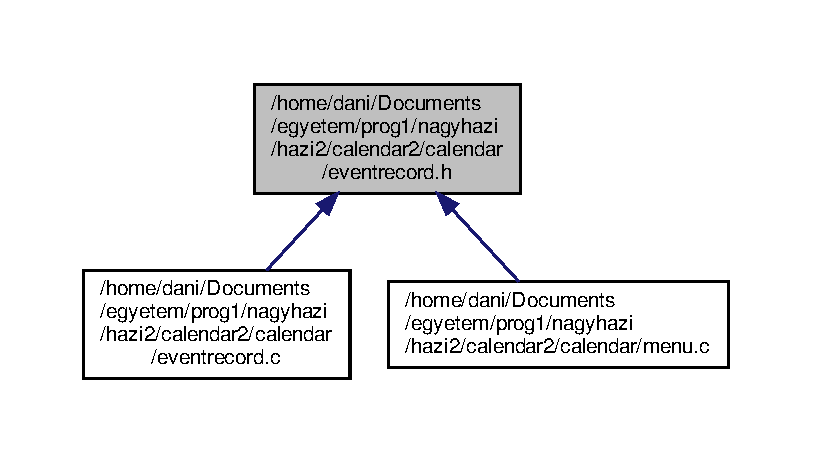
\includegraphics[width=350pt]{eventrecord_8h__dep__incl}
\end{center}
\end{figure}

\hypertarget{file_8c}{}\section{/home/dani/\+Documents/egyetem/prog1/nagyhazi/hazi2/calendar2/calendar/file.c File Reference}
\label{file_8c}\index{/home/dani/\+Documents/egyetem/prog1/nagyhazi/hazi2/calendar2/calendar/file.\+c@{/home/dani/\+Documents/egyetem/prog1/nagyhazi/hazi2/calendar2/calendar/file.\+c}}
{\ttfamily \#include \char`\"{}file.\+h\char`\"{}}\newline
{\ttfamily \#include $<$stdio.\+h$>$}\newline
{\ttfamily \#include $<$stdbool.\+h$>$}\newline
{\ttfamily \#include \char`\"{}structures.\+h\char`\"{}}\newline
{\ttfamily \#include \char`\"{}list.\+h\char`\"{}}\newline
{\ttfamily \#include $<$string.\+h$>$}\newline
{\ttfamily \#include $<$stdlib.\+h$>$}\newline
\subsection*{Functions}
\begin{DoxyCompactItemize}
\item 
char $\ast$ \hyperlink{group__file_ga91b52505951ff88321e947b6e1c4b779}{dstrcpy} (char const $\ast$str)
\item 
bool \hyperlink{group__file_gaf4efa1e078c7552b2f70daf3a40039c7}{calendarload} (\hyperlink{struct_event_list}{Event\+List} const $\ast$eventlist)
\item 
bool \hyperlink{group__file_ga7f69872489b7c1c4bcdd125319a87b2e}{calendarsave} (\hyperlink{struct_event_list}{Event\+List} const $\ast$eventlist)
\end{DoxyCompactItemize}

\hypertarget{file_8h}{}\section{/home/dani/\+Documents/egyetem/prog1/nagyhazi/hazi2/calendar2/calendar/file.h File Reference}
\label{file_8h}\index{/home/dani/\+Documents/egyetem/prog1/nagyhazi/hazi2/calendar2/calendar/file.\+h@{/home/dani/\+Documents/egyetem/prog1/nagyhazi/hazi2/calendar2/calendar/file.\+h}}
{\ttfamily \#include $<$stdio.\+h$>$}\newline
{\ttfamily \#include \char`\"{}structures.\+h\char`\"{}}\newline
Include dependency graph for file.\+h\+:\nopagebreak
\begin{figure}[H]
\begin{center}
\leavevmode
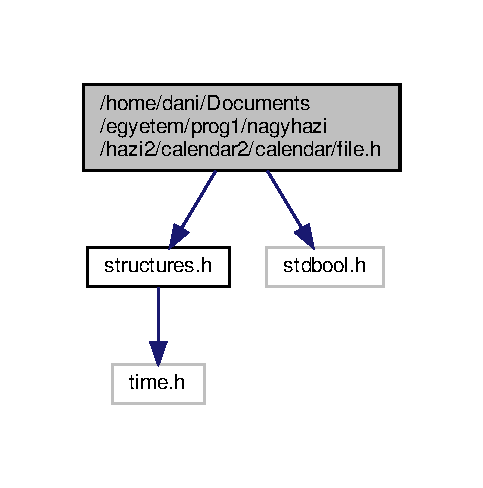
\includegraphics[width=232pt]{file_8h__incl}
\end{center}
\end{figure}
This graph shows which files directly or indirectly include this file\+:\nopagebreak
\begin{figure}[H]
\begin{center}
\leavevmode
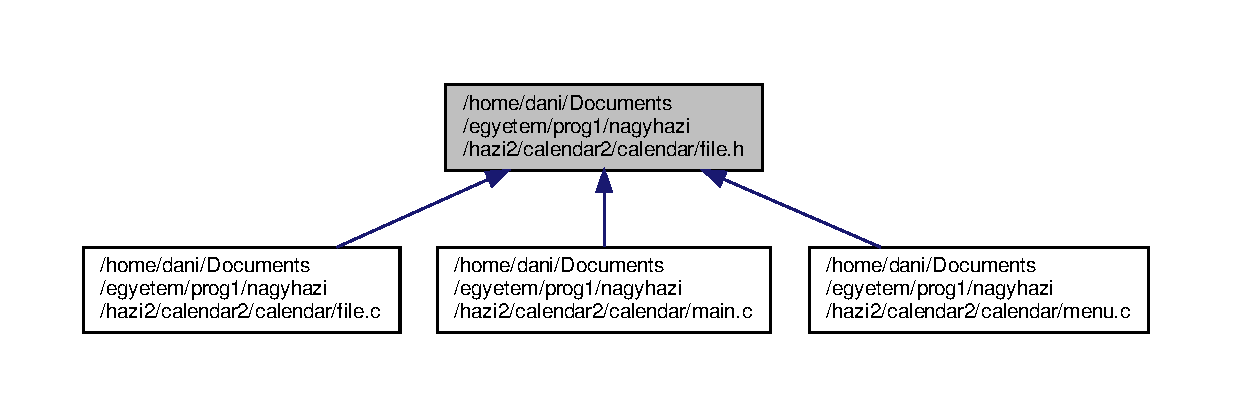
\includegraphics[width=350pt]{file_8h__dep__incl}
\end{center}
\end{figure}
\subsection*{Functions}
\begin{DoxyCompactItemize}
\item 
void \hyperlink{file_8h_a31d677237f8b1f618a6183133eae616d}{fileload} ()
\item 
void \hyperlink{file_8h_afc715bc6c0b9a9e85af15dc509a8d34b}{filesave} (\hyperlink{struct_event_list}{Event\+List} $\ast$eventlist)
\end{DoxyCompactItemize}


\subsection{Function Documentation}
\mbox{\Hypertarget{file_8h_a31d677237f8b1f618a6183133eae616d}\label{file_8h_a31d677237f8b1f618a6183133eae616d}} 
\index{file.\+h@{file.\+h}!fileload@{fileload}}
\index{fileload@{fileload}!file.\+h@{file.\+h}}
\subsubsection{\texorpdfstring{fileload()}{fileload()}}
{\footnotesize\ttfamily void fileload (\begin{DoxyParamCaption}{ }\end{DoxyParamCaption})}

\mbox{\Hypertarget{file_8h_afc715bc6c0b9a9e85af15dc509a8d34b}\label{file_8h_afc715bc6c0b9a9e85af15dc509a8d34b}} 
\index{file.\+h@{file.\+h}!filesave@{filesave}}
\index{filesave@{filesave}!file.\+h@{file.\+h}}
\subsubsection{\texorpdfstring{filesave()}{filesave()}}
{\footnotesize\ttfamily void filesave (\begin{DoxyParamCaption}\item[{\hyperlink{struct_event_list}{Event\+List} $\ast$}]{eventlist }\end{DoxyParamCaption})}

Here is the call graph for this function\+:
\nopagebreak
\begin{figure}[H]
\begin{center}
\leavevmode
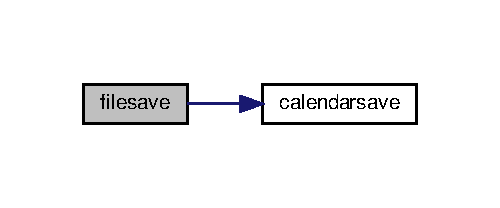
\includegraphics[width=240pt]{file_8h_afc715bc6c0b9a9e85af15dc509a8d34b_cgraph}
\end{center}
\end{figure}
Here is the caller graph for this function\+:
\nopagebreak
\begin{figure}[H]
\begin{center}
\leavevmode
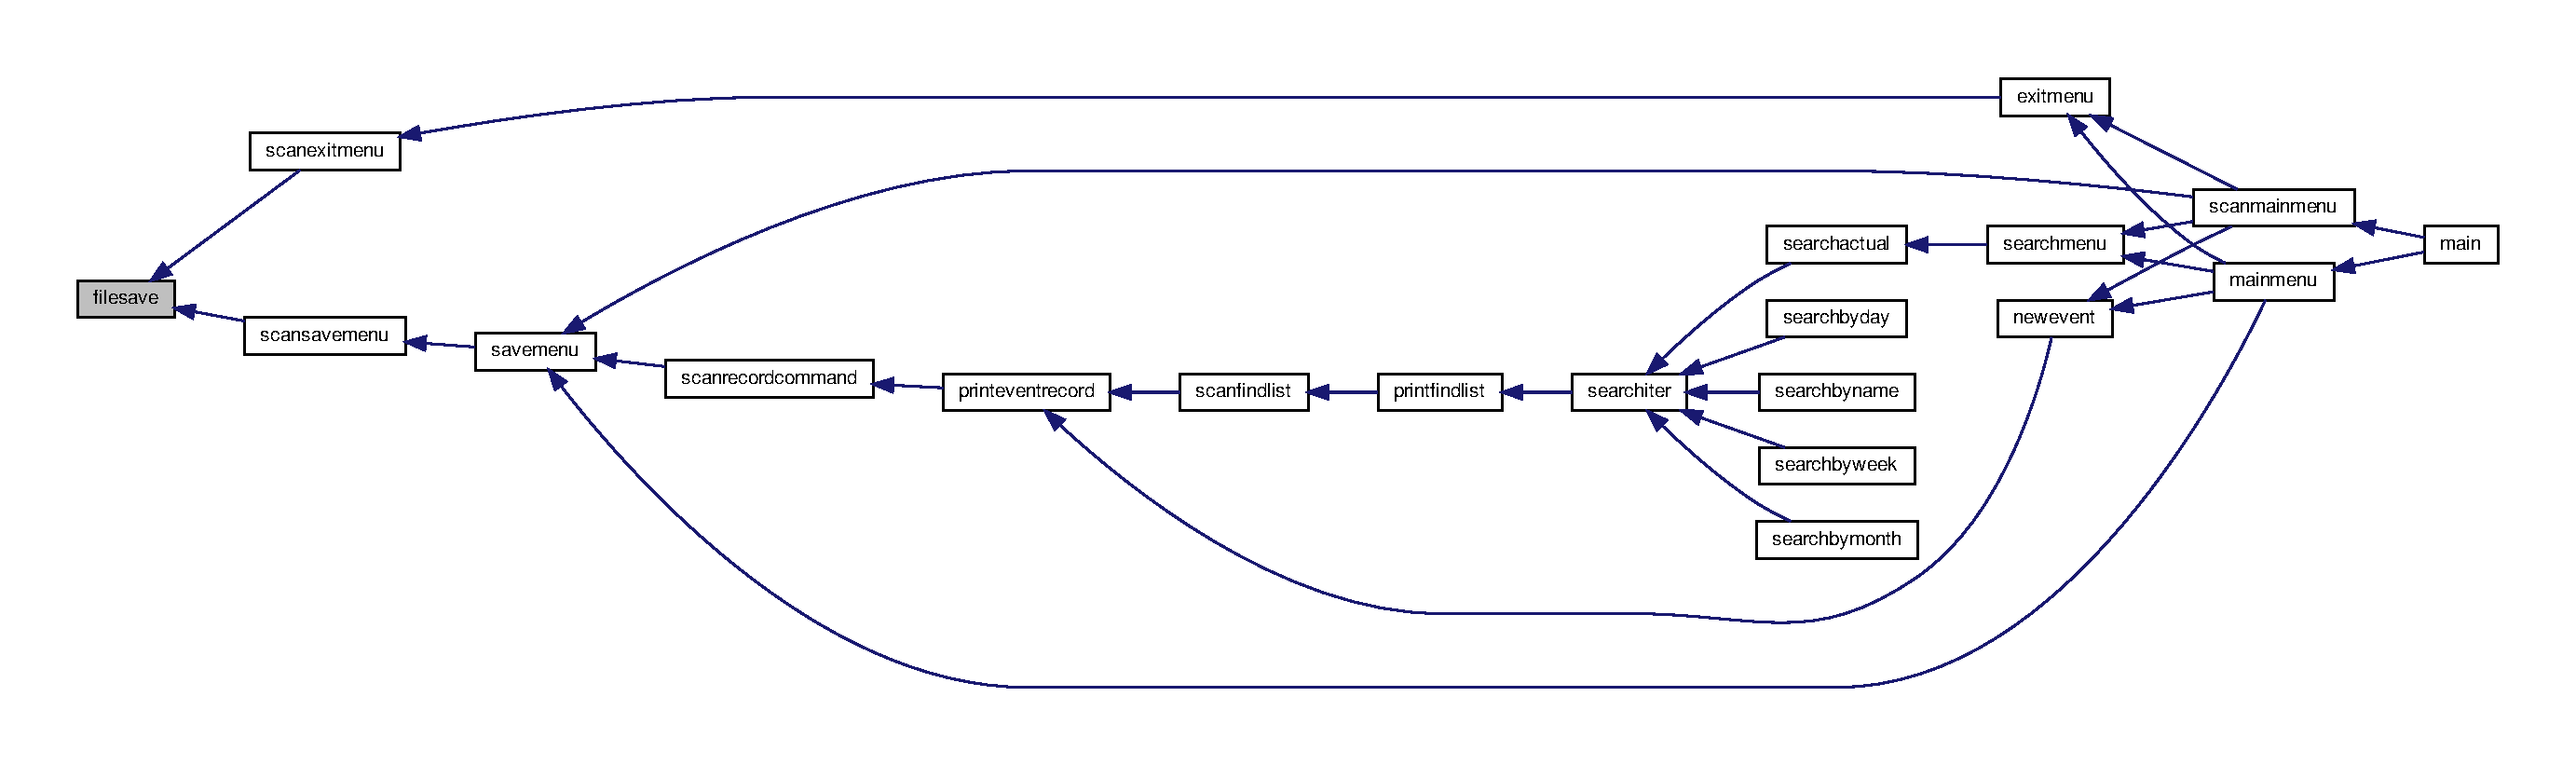
\includegraphics[width=350pt]{file_8h_afc715bc6c0b9a9e85af15dc509a8d34b_icgraph}
\end{center}
\end{figure}

\hypertarget{list_8c}{}\section{/home/dani/\+Documents/egyetem/prog1/nagyhazi/hazi2/calendar2/calendar/list.c File Reference}
\label{list_8c}\index{/home/dani/\+Documents/egyetem/prog1/nagyhazi/hazi2/calendar2/calendar/list.\+c@{/home/dani/\+Documents/egyetem/prog1/nagyhazi/hazi2/calendar2/calendar/list.\+c}}
{\ttfamily \#include \char`\"{}list.\+h\char`\"{}}\newline
{\ttfamily \#include $<$stdlib.\+h$>$}\newline
{\ttfamily \#include \char`\"{}structures.\+h\char`\"{}}\newline
{\ttfamily \#include $<$time.\+h$>$}\newline
Include dependency graph for list.\+c\+:\nopagebreak
\begin{figure}[H]
\begin{center}
\leavevmode
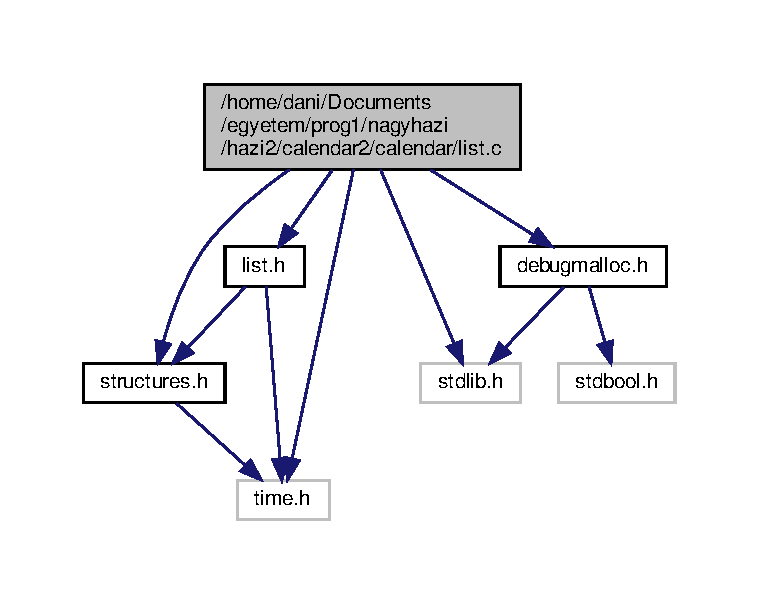
\includegraphics[width=290pt]{list_8c__incl}
\end{center}
\end{figure}
\subsection*{Functions}
\begin{DoxyCompactItemize}
\item 
\hyperlink{struct_event_list}{Event\+List} $\ast$ \hyperlink{list_8c_a48f44148563512bd32274821f478bd1b}{initeventlist} ()
\item 
\hyperlink{struct_event}{Event} $\ast$ \hyperlink{list_8c_a24fd1b37eee54600b66c42e86b52244a}{createevent} (int ev, int honap, int nap, int ora, int perc, int bora, int bperc, char $\ast$nev, char $\ast$hely, char $\ast$comment)
\item 
void \hyperlink{list_8c_a7ef519287e473ee333204280a5d91403}{insertevent} (\hyperlink{struct_event_list}{Event\+List} $\ast$eventlist, \hyperlink{struct_event}{Event} $\ast$event)
\item 
int \hyperlink{list_8c_a8f7708495c6e39bb6e712218711b331f}{starttime} (\hyperlink{struct_event}{Event} $\ast$event)
\item 
void \hyperlink{list_8c_a2561d96be1299fd3f5730c6d82143709}{printevent\+\_\+short} (\hyperlink{struct_event}{Event} $\ast$event)
\end{DoxyCompactItemize}


\subsection{Function Documentation}
\mbox{\Hypertarget{list_8c_a24fd1b37eee54600b66c42e86b52244a}\label{list_8c_a24fd1b37eee54600b66c42e86b52244a}} 
\index{list.\+c@{list.\+c}!createevent@{createevent}}
\index{createevent@{createevent}!list.\+c@{list.\+c}}
\subsubsection{\texorpdfstring{createevent()}{createevent()}}
{\footnotesize\ttfamily \hyperlink{struct_event}{Event}$\ast$ createevent (\begin{DoxyParamCaption}\item[{int}]{ev,  }\item[{int}]{honap,  }\item[{int}]{nap,  }\item[{int}]{ora,  }\item[{int}]{perc,  }\item[{int}]{bora,  }\item[{int}]{bperc,  }\item[{char $\ast$}]{nev,  }\item[{char $\ast$}]{hely,  }\item[{char $\ast$}]{comment }\end{DoxyParamCaption})}

Here is the caller graph for this function\+:
\nopagebreak
\begin{figure}[H]
\begin{center}
\leavevmode
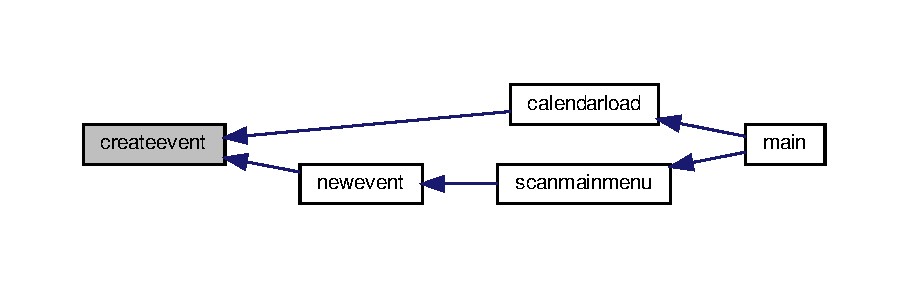
\includegraphics[width=350pt]{list_8c_a24fd1b37eee54600b66c42e86b52244a_icgraph}
\end{center}
\end{figure}
\mbox{\Hypertarget{list_8c_a48f44148563512bd32274821f478bd1b}\label{list_8c_a48f44148563512bd32274821f478bd1b}} 
\index{list.\+c@{list.\+c}!initeventlist@{initeventlist}}
\index{initeventlist@{initeventlist}!list.\+c@{list.\+c}}
\subsubsection{\texorpdfstring{initeventlist()}{initeventlist()}}
{\footnotesize\ttfamily \hyperlink{struct_event_list}{Event\+List}$\ast$ initeventlist (\begin{DoxyParamCaption}{ }\end{DoxyParamCaption})}

Here is the caller graph for this function\+:
\nopagebreak
\begin{figure}[H]
\begin{center}
\leavevmode
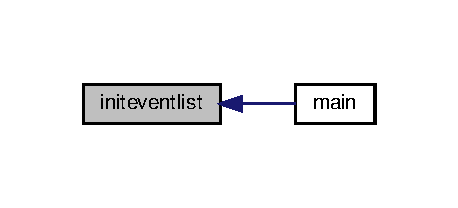
\includegraphics[width=220pt]{list_8c_a48f44148563512bd32274821f478bd1b_icgraph}
\end{center}
\end{figure}
\mbox{\Hypertarget{list_8c_a7ef519287e473ee333204280a5d91403}\label{list_8c_a7ef519287e473ee333204280a5d91403}} 
\index{list.\+c@{list.\+c}!insertevent@{insertevent}}
\index{insertevent@{insertevent}!list.\+c@{list.\+c}}
\subsubsection{\texorpdfstring{insertevent()}{insertevent()}}
{\footnotesize\ttfamily void insertevent (\begin{DoxyParamCaption}\item[{\hyperlink{struct_event_list}{Event\+List} $\ast$}]{eventlist,  }\item[{\hyperlink{struct_event}{Event} $\ast$}]{event }\end{DoxyParamCaption})}

Here is the call graph for this function\+:
\nopagebreak
\begin{figure}[H]
\begin{center}
\leavevmode
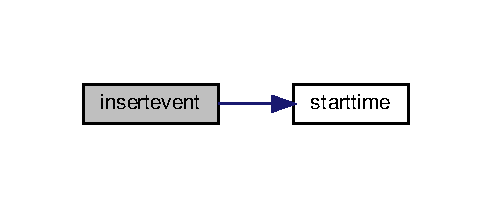
\includegraphics[width=236pt]{list_8c_a7ef519287e473ee333204280a5d91403_cgraph}
\end{center}
\end{figure}
Here is the caller graph for this function\+:
\nopagebreak
\begin{figure}[H]
\begin{center}
\leavevmode
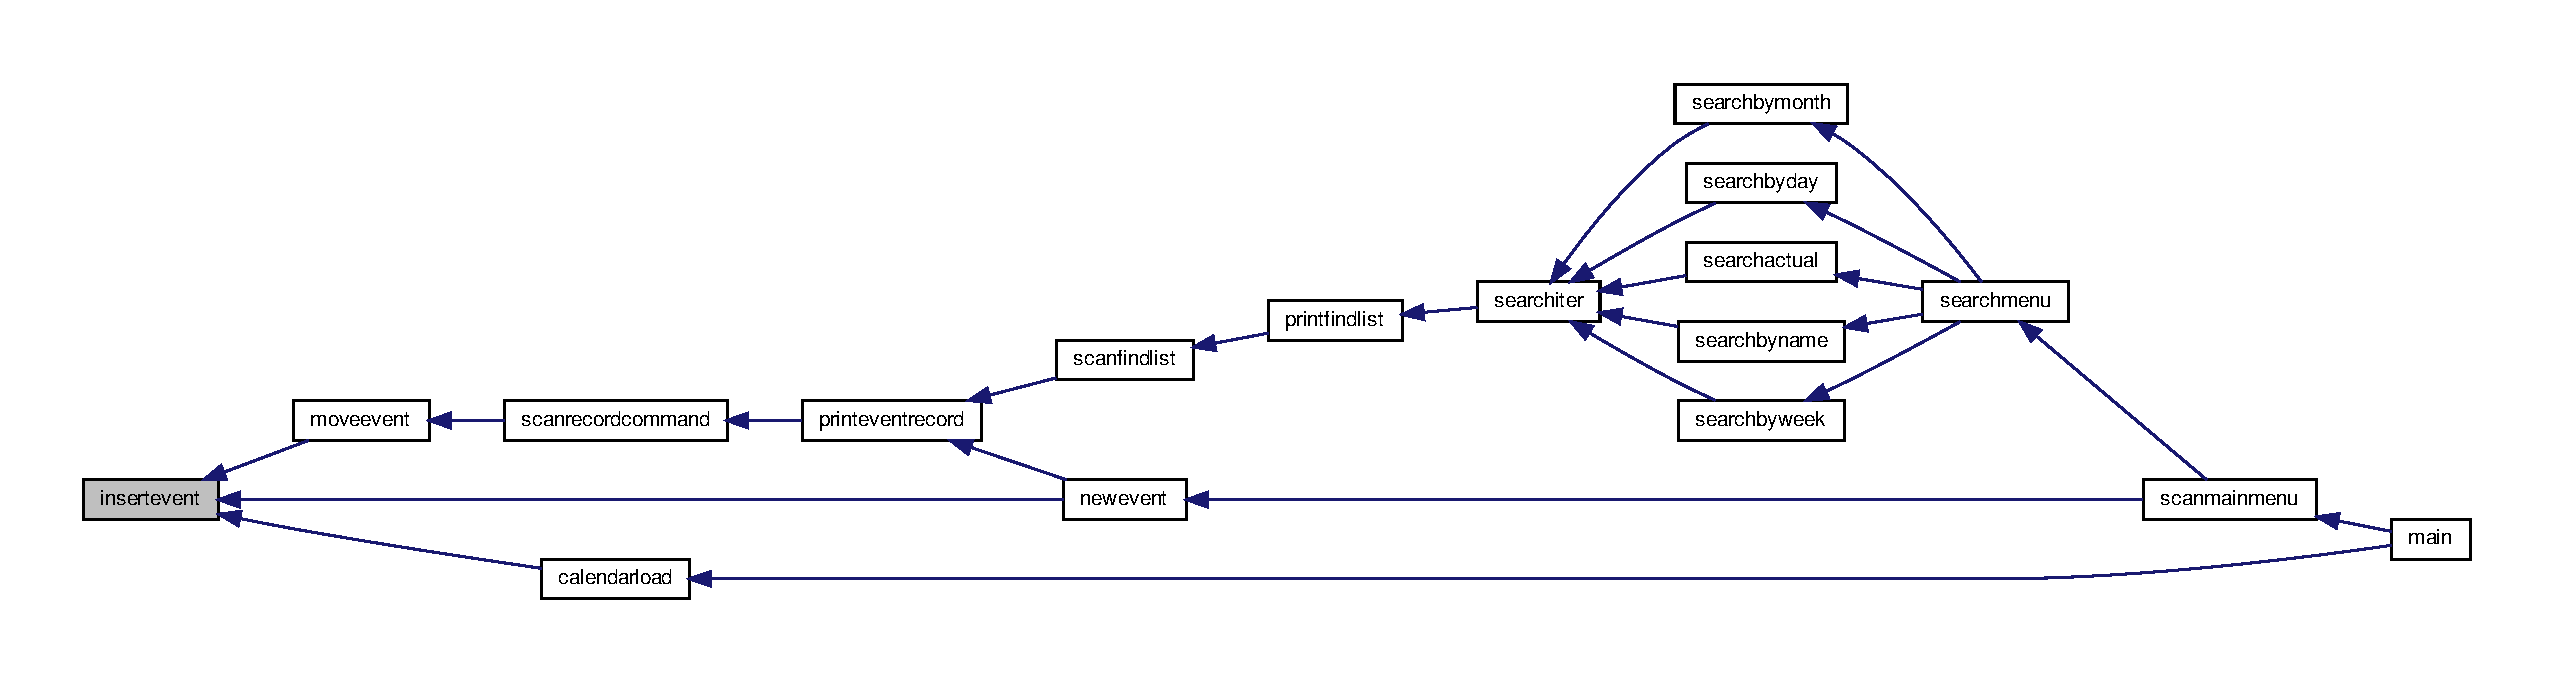
\includegraphics[width=350pt]{list_8c_a7ef519287e473ee333204280a5d91403_icgraph}
\end{center}
\end{figure}
\mbox{\Hypertarget{list_8c_a2561d96be1299fd3f5730c6d82143709}\label{list_8c_a2561d96be1299fd3f5730c6d82143709}} 
\index{list.\+c@{list.\+c}!printevent\+\_\+short@{printevent\+\_\+short}}
\index{printevent\+\_\+short@{printevent\+\_\+short}!list.\+c@{list.\+c}}
\subsubsection{\texorpdfstring{printevent\+\_\+short()}{printevent\_short()}}
{\footnotesize\ttfamily void printevent\+\_\+short (\begin{DoxyParamCaption}\item[{\hyperlink{struct_event}{Event} $\ast$}]{event }\end{DoxyParamCaption})}

Here is the caller graph for this function\+:
\nopagebreak
\begin{figure}[H]
\begin{center}
\leavevmode
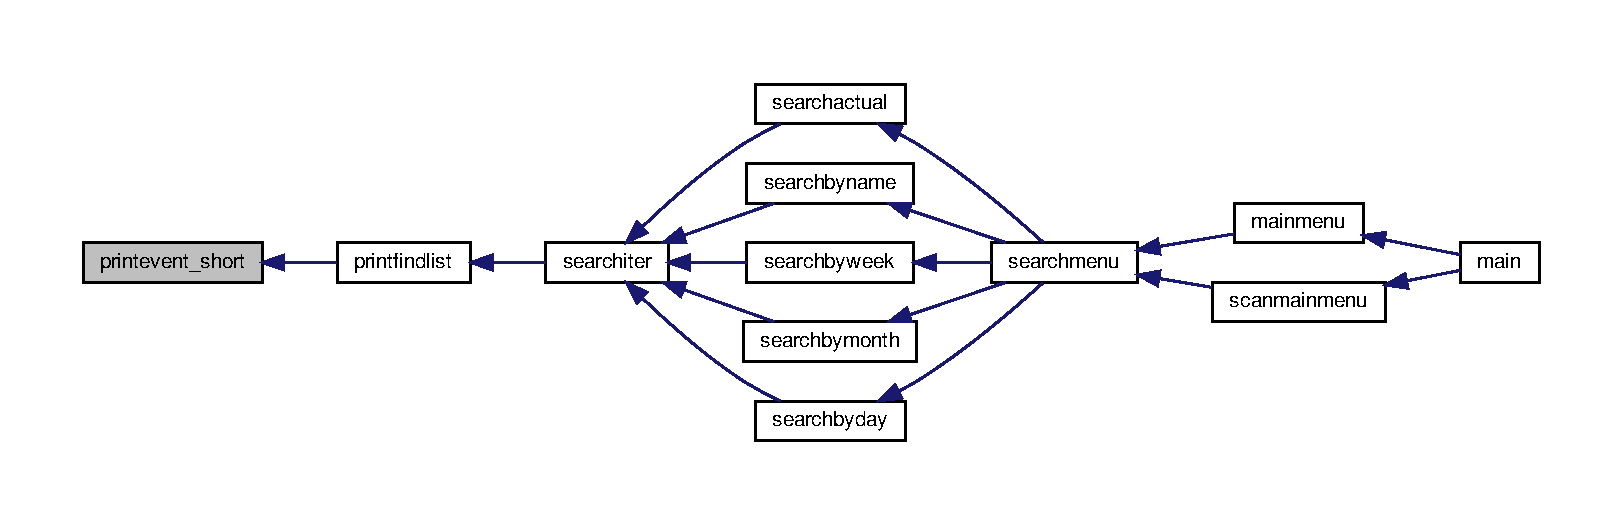
\includegraphics[width=350pt]{list_8c_a2561d96be1299fd3f5730c6d82143709_icgraph}
\end{center}
\end{figure}
\mbox{\Hypertarget{list_8c_a8f7708495c6e39bb6e712218711b331f}\label{list_8c_a8f7708495c6e39bb6e712218711b331f}} 
\index{list.\+c@{list.\+c}!starttime@{starttime}}
\index{starttime@{starttime}!list.\+c@{list.\+c}}
\subsubsection{\texorpdfstring{starttime()}{starttime()}}
{\footnotesize\ttfamily int starttime (\begin{DoxyParamCaption}\item[{\hyperlink{struct_event}{Event} $\ast$}]{event }\end{DoxyParamCaption})}

Here is the caller graph for this function\+:
\nopagebreak
\begin{figure}[H]
\begin{center}
\leavevmode
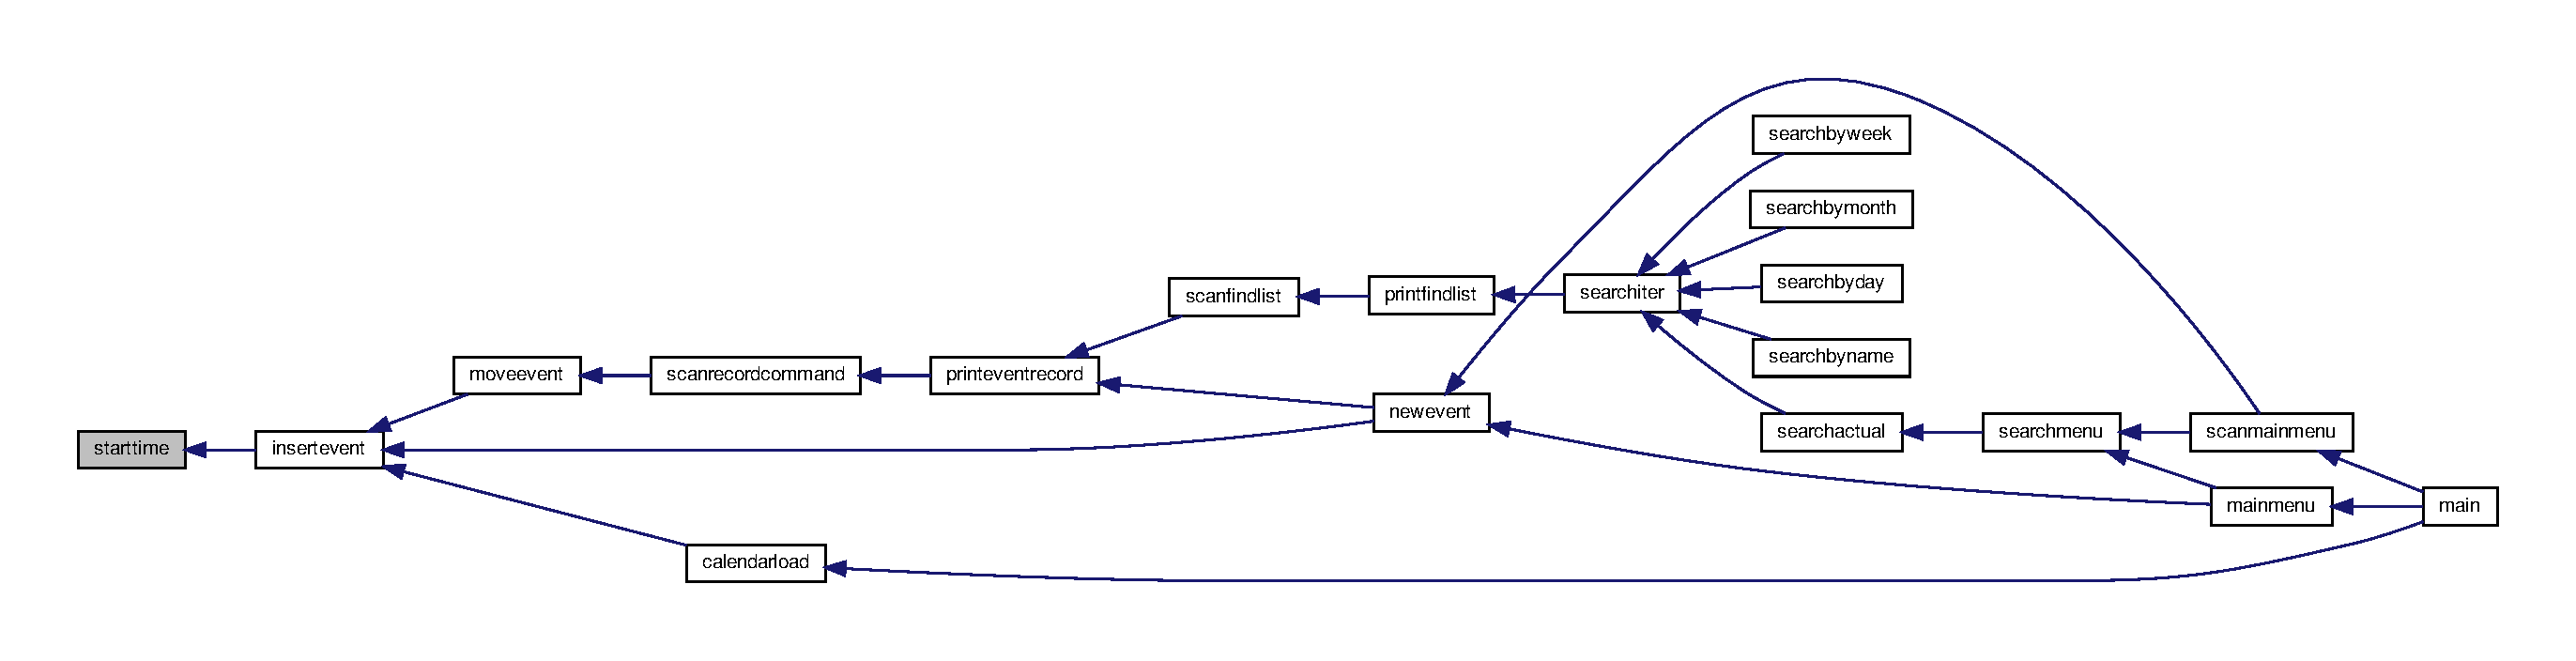
\includegraphics[width=350pt]{list_8c_a8f7708495c6e39bb6e712218711b331f_icgraph}
\end{center}
\end{figure}

\hypertarget{list_8h}{}\section{/home/dani/\+Documents/egyetem/prog1/nagyhazi/hazi2/calendar2/calendar/list.h File Reference}
\label{list_8h}\index{/home/dani/\+Documents/egyetem/prog1/nagyhazi/hazi2/calendar2/calendar/list.\+h@{/home/dani/\+Documents/egyetem/prog1/nagyhazi/hazi2/calendar2/calendar/list.\+h}}
{\ttfamily \#include \char`\"{}structures.\+h\char`\"{}}\newline
{\ttfamily \#include $<$time.\+h$>$}\newline
Include dependency graph for list.\+h\+:\nopagebreak
\begin{figure}[H]
\begin{center}
\leavevmode
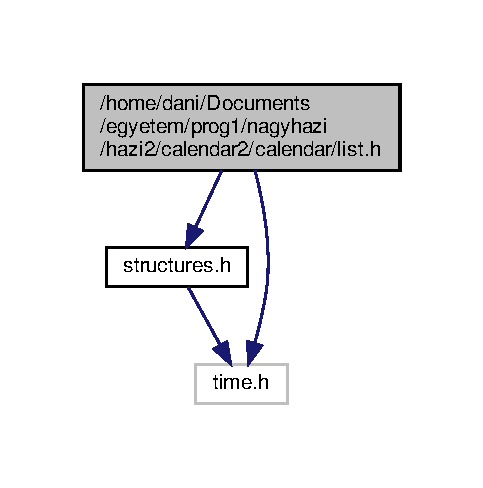
\includegraphics[width=232pt]{list_8h__incl}
\end{center}
\end{figure}
This graph shows which files directly or indirectly include this file\+:
\nopagebreak
\begin{figure}[H]
\begin{center}
\leavevmode
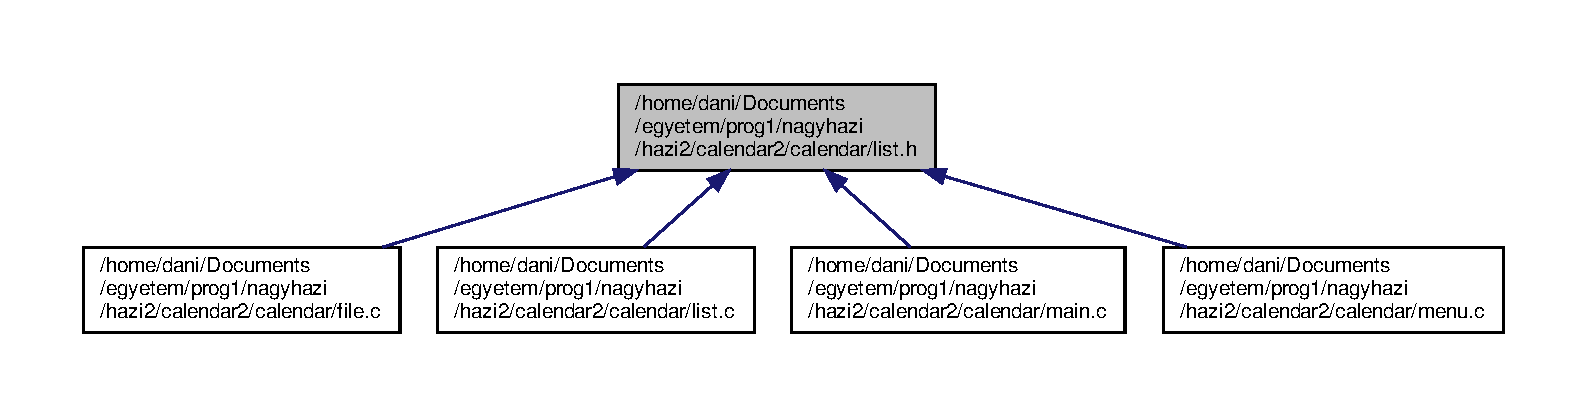
\includegraphics[width=350pt]{list_8h__dep__incl}
\end{center}
\end{figure}
\subsection*{Typedefs}
\begin{DoxyCompactItemize}
\item 
typedef struct tm \hyperlink{list_8h_affc453d30a4a6ce81ed778fd04d2d256}{Tm}
\end{DoxyCompactItemize}
\subsection*{Functions}
\begin{DoxyCompactItemize}
\item 
\hyperlink{struct_event_list}{Event\+List} $\ast$ \hyperlink{list_8h_a48f44148563512bd32274821f478bd1b}{initeventlist} ()
\item 
void \hyperlink{list_8h_a2561d96be1299fd3f5730c6d82143709}{printevent\+\_\+short} (\hyperlink{struct_event}{Event} $\ast$event)
\item 
void \hyperlink{list_8h_a7ef519287e473ee333204280a5d91403}{insertevent} (\hyperlink{struct_event_list}{Event\+List} $\ast$eventlist, \hyperlink{struct_event}{Event} $\ast$event)
\item 
\hyperlink{struct_event}{Event} $\ast$ \hyperlink{list_8h_a24fd1b37eee54600b66c42e86b52244a}{createevent} (int ev, int honap, int nap, int ora, int perc, int bora, int bperc, char $\ast$nev, char $\ast$hely, char $\ast$comment)
\end{DoxyCompactItemize}


\subsection{Typedef Documentation}
\mbox{\Hypertarget{list_8h_affc453d30a4a6ce81ed778fd04d2d256}\label{list_8h_affc453d30a4a6ce81ed778fd04d2d256}} 
\index{list.\+h@{list.\+h}!Tm@{Tm}}
\index{Tm@{Tm}!list.\+h@{list.\+h}}
\subsubsection{\texorpdfstring{Tm}{Tm}}
{\footnotesize\ttfamily typedef struct tm \hyperlink{list_8h_affc453d30a4a6ce81ed778fd04d2d256}{Tm}}



\subsection{Function Documentation}
\mbox{\Hypertarget{list_8h_a24fd1b37eee54600b66c42e86b52244a}\label{list_8h_a24fd1b37eee54600b66c42e86b52244a}} 
\index{list.\+h@{list.\+h}!createevent@{createevent}}
\index{createevent@{createevent}!list.\+h@{list.\+h}}
\subsubsection{\texorpdfstring{createevent()}{createevent()}}
{\footnotesize\ttfamily \hyperlink{struct_event}{Event}$\ast$ createevent (\begin{DoxyParamCaption}\item[{int}]{ev,  }\item[{int}]{honap,  }\item[{int}]{nap,  }\item[{int}]{ora,  }\item[{int}]{perc,  }\item[{int}]{bora,  }\item[{int}]{bperc,  }\item[{char $\ast$}]{nev,  }\item[{char $\ast$}]{hely,  }\item[{char $\ast$}]{comment }\end{DoxyParamCaption})}

Here is the caller graph for this function\+:
\nopagebreak
\begin{figure}[H]
\begin{center}
\leavevmode
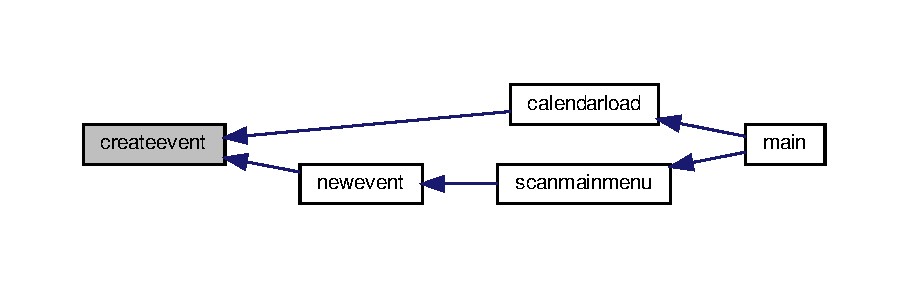
\includegraphics[width=350pt]{list_8h_a24fd1b37eee54600b66c42e86b52244a_icgraph}
\end{center}
\end{figure}
\mbox{\Hypertarget{list_8h_a48f44148563512bd32274821f478bd1b}\label{list_8h_a48f44148563512bd32274821f478bd1b}} 
\index{list.\+h@{list.\+h}!initeventlist@{initeventlist}}
\index{initeventlist@{initeventlist}!list.\+h@{list.\+h}}
\subsubsection{\texorpdfstring{initeventlist()}{initeventlist()}}
{\footnotesize\ttfamily \hyperlink{struct_event_list}{Event\+List}$\ast$ initeventlist (\begin{DoxyParamCaption}{ }\end{DoxyParamCaption})}

Here is the caller graph for this function\+:
\nopagebreak
\begin{figure}[H]
\begin{center}
\leavevmode
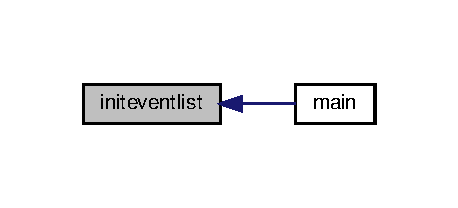
\includegraphics[width=220pt]{list_8h_a48f44148563512bd32274821f478bd1b_icgraph}
\end{center}
\end{figure}
\mbox{\Hypertarget{list_8h_a7ef519287e473ee333204280a5d91403}\label{list_8h_a7ef519287e473ee333204280a5d91403}} 
\index{list.\+h@{list.\+h}!insertevent@{insertevent}}
\index{insertevent@{insertevent}!list.\+h@{list.\+h}}
\subsubsection{\texorpdfstring{insertevent()}{insertevent()}}
{\footnotesize\ttfamily void insertevent (\begin{DoxyParamCaption}\item[{\hyperlink{struct_event_list}{Event\+List} $\ast$}]{eventlist,  }\item[{\hyperlink{struct_event}{Event} $\ast$}]{event }\end{DoxyParamCaption})}

Here is the call graph for this function\+:
\nopagebreak
\begin{figure}[H]
\begin{center}
\leavevmode
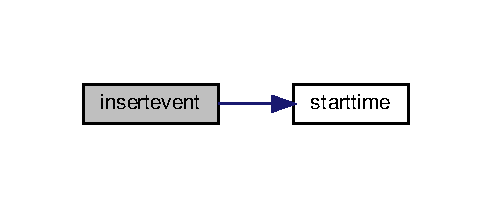
\includegraphics[width=236pt]{list_8h_a7ef519287e473ee333204280a5d91403_cgraph}
\end{center}
\end{figure}
Here is the caller graph for this function\+:
\nopagebreak
\begin{figure}[H]
\begin{center}
\leavevmode
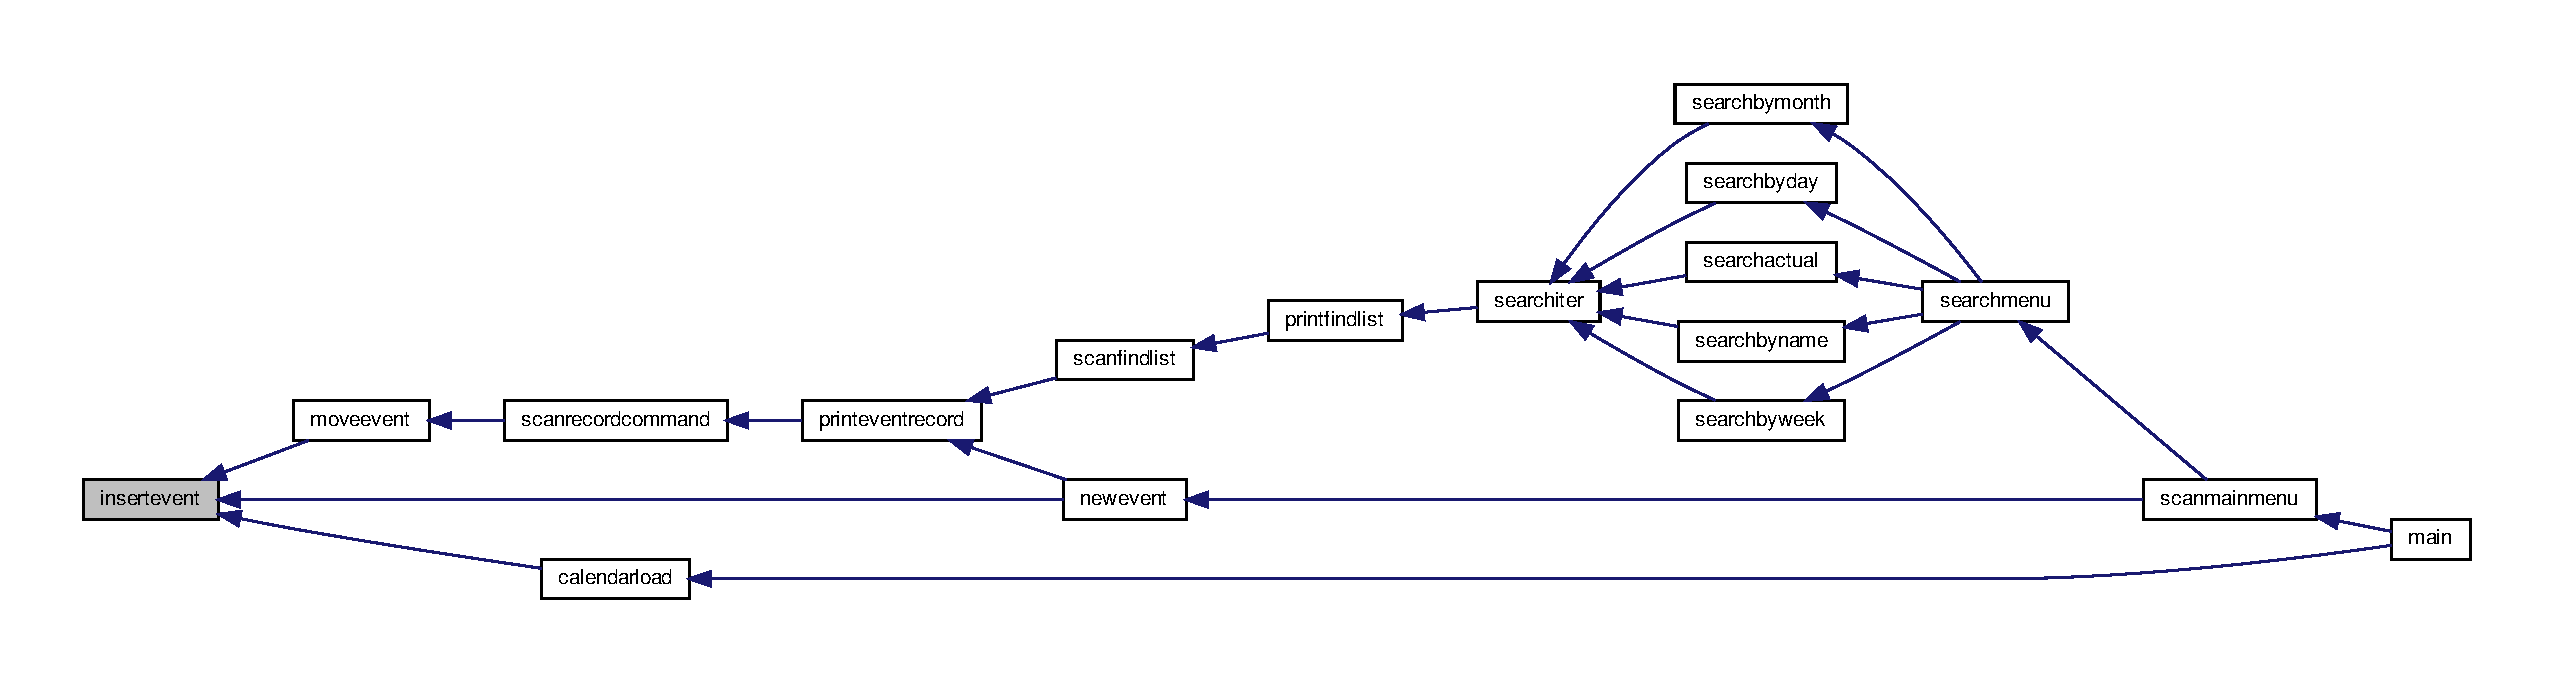
\includegraphics[width=350pt]{list_8h_a7ef519287e473ee333204280a5d91403_icgraph}
\end{center}
\end{figure}
\mbox{\Hypertarget{list_8h_a2561d96be1299fd3f5730c6d82143709}\label{list_8h_a2561d96be1299fd3f5730c6d82143709}} 
\index{list.\+h@{list.\+h}!printevent\+\_\+short@{printevent\+\_\+short}}
\index{printevent\+\_\+short@{printevent\+\_\+short}!list.\+h@{list.\+h}}
\subsubsection{\texorpdfstring{printevent\+\_\+short()}{printevent\_short()}}
{\footnotesize\ttfamily void printevent\+\_\+short (\begin{DoxyParamCaption}\item[{\hyperlink{struct_event}{Event} $\ast$}]{event }\end{DoxyParamCaption})}

Here is the caller graph for this function\+:
\nopagebreak
\begin{figure}[H]
\begin{center}
\leavevmode
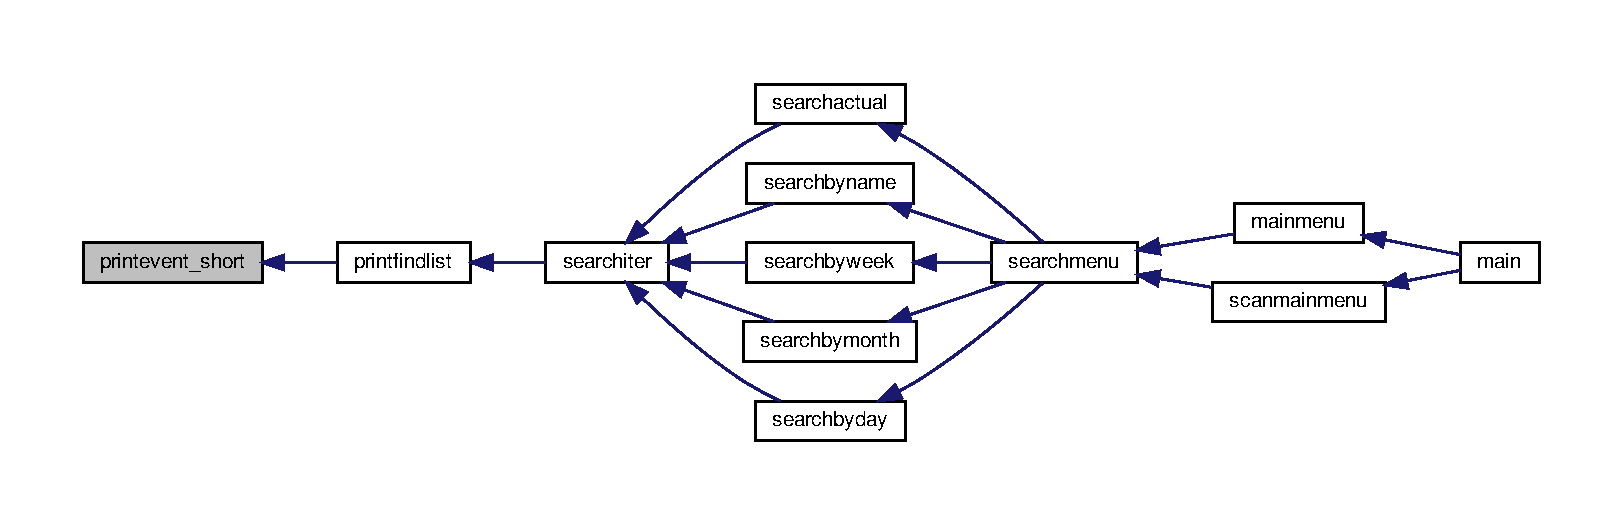
\includegraphics[width=350pt]{list_8h_a2561d96be1299fd3f5730c6d82143709_icgraph}
\end{center}
\end{figure}

\hypertarget{main_8c}{}\section{/home/dani/\+Documents/egyetem/prog1/nagyhazi/hazi2/calendar2/calendar/main.c File Reference}
\label{main_8c}\index{/home/dani/\+Documents/egyetem/prog1/nagyhazi/hazi2/calendar2/calendar/main.\+c@{/home/dani/\+Documents/egyetem/prog1/nagyhazi/hazi2/calendar2/calendar/main.\+c}}
{\ttfamily \#include $<$stdio.\+h$>$}\newline
{\ttfamily \#include $<$stdlib.\+h$>$}\newline
{\ttfamily \#include \char`\"{}structures.\+h\char`\"{}}\newline
{\ttfamily \#include \char`\"{}file.\+h\char`\"{}}\newline
{\ttfamily \#include \char`\"{}list.\+h\char`\"{}}\newline
{\ttfamily \#include \char`\"{}menu.\+h\char`\"{}}\newline
{\ttfamily \#include $<$stdbool.\+h$>$}\newline
{\ttfamily \#include \char`\"{}debugmalloc.\+h\char`\"{}}\newline
\subsection*{Functions}
\begin{DoxyCompactItemize}
\item 
int \hyperlink{main_8c_ae66f6b31b5ad750f1fe042a706a4e3d4}{main} ()
\end{DoxyCompactItemize}


\subsection{Function Documentation}
\mbox{\Hypertarget{main_8c_ae66f6b31b5ad750f1fe042a706a4e3d4}\label{main_8c_ae66f6b31b5ad750f1fe042a706a4e3d4}} 
\index{main.\+c@{main.\+c}!main@{main}}
\index{main@{main}!main.\+c@{main.\+c}}
\subsubsection{\texorpdfstring{main()}{main()}}
{\footnotesize\ttfamily int main (\begin{DoxyParamCaption}{ }\end{DoxyParamCaption})}


\hypertarget{menu_8c}{}\section{/home/dani/\+Documents/egyetem/prog1/nagyhazi/hazi2/calendar2/calendar/menu.c File Reference}
\label{menu_8c}\index{/home/dani/\+Documents/egyetem/prog1/nagyhazi/hazi2/calendar2/calendar/menu.\+c@{/home/dani/\+Documents/egyetem/prog1/nagyhazi/hazi2/calendar2/calendar/menu.\+c}}
{\ttfamily \#include \char`\"{}menu.\+h\char`\"{}}\newline
{\ttfamily \#include \char`\"{}structures.\+h\char`\"{}}\newline
{\ttfamily \#include $<$stdlib.\+h$>$}\newline
{\ttfamily \#include \char`\"{}file.\+h\char`\"{}}\newline
{\ttfamily \#include $<$stdio.\+h$>$}\newline
{\ttfamily \#include $<$string.\+h$>$}\newline
{\ttfamily \#include $<$stdbool.\+h$>$}\newline
Include dependency graph for menu.\+c\+:\nopagebreak
\begin{figure}[H]
\begin{center}
\leavevmode
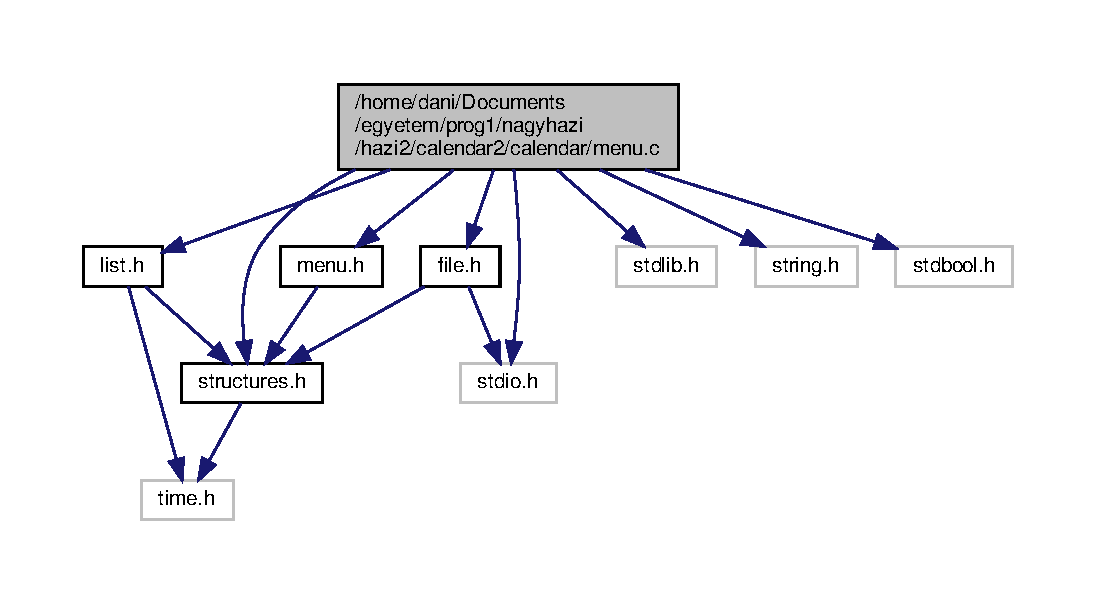
\includegraphics[width=350pt]{menu_8c__incl}
\end{center}
\end{figure}
\subsection*{Functions}
\begin{DoxyCompactItemize}
\item 
void \hyperlink{menu_8c_afc715bc6c0b9a9e85af15dc509a8d34b}{filesave} (\hyperlink{struct_event_list}{Event\+List} $\ast$eventlist)
\item 
void \hyperlink{menu_8c_ac2c3136ef241a7150d7cff391a0eb048}{newevent} (\hyperlink{struct_event_list}{Event\+List} $\ast$eventlist)
\item 
char $\ast$ \hyperlink{menu_8c_ab9ac014b764791c1dc71c187dca898f7}{hosszu\+\_\+sort\+\_\+olvas} (int bufferhossz)
\item 
void \hyperlink{menu_8c_ac86d3169260f5cacd0f792743957b054}{mainmenu} ()
\item 
void \hyperlink{menu_8c_a8e572ab27981dcd7144340fd25a24c80}{scanmainmenu} (\hyperlink{struct_event_list}{Event\+List} $\ast$eventlist)
\item 
void \hyperlink{menu_8c_a38d64ff02f60ebcb1988655ea12540a6}{searchmenu} (\hyperlink{struct_event_list}{Event\+List} $\ast$eventlist)
\item 
void \hyperlink{menu_8c_aa28daf84be098b64b8dfea8a88050f13}{savemenu} (\hyperlink{struct_event_list}{Event\+List} $\ast$eventlist)
\item 
int \hyperlink{menu_8c_a6ef5647864065ede4ef3b2773cbb9e8d}{scansavemenu} (\hyperlink{struct_event_list}{Event\+List} $\ast$eventlist)
\item 
void \hyperlink{menu_8c_ac651d3838f4da7bf6055fa839621e289}{exitmenu} (\hyperlink{struct_event_list}{Event\+List} $\ast$eventlist)
\item 
int \hyperlink{menu_8c_aa12eba16d2e2bd5dfc70240d19bd5c8e}{scanexitmenu} (\hyperlink{struct_event_list}{Event\+List} $\ast$eventlist)
\item 
int \hyperlink{menu_8c_a1aa7ba6b6941a272c34eea491e4a650d}{printmenu} (\hyperlink{struct_menu_pont}{Menu\+Pont} $\ast$menupontok)
\item 
void \hyperlink{menu_8c_a00af175f266f31d352be878cfb5d5640}{callmenu} (int meret, \hyperlink{struct_menu_pont}{Menu\+Pont} $\ast$menupontok, \hyperlink{struct_event_list}{Event\+List} $\ast$eventlist)
\end{DoxyCompactItemize}


\subsection{Function Documentation}
\mbox{\Hypertarget{menu_8c_a00af175f266f31d352be878cfb5d5640}\label{menu_8c_a00af175f266f31d352be878cfb5d5640}} 
\index{menu.\+c@{menu.\+c}!callmenu@{callmenu}}
\index{callmenu@{callmenu}!menu.\+c@{menu.\+c}}
\subsubsection{\texorpdfstring{callmenu()}{callmenu()}}
{\footnotesize\ttfamily void callmenu (\begin{DoxyParamCaption}\item[{int}]{meret,  }\item[{\hyperlink{struct_menu_pont}{Menu\+Pont} $\ast$}]{menupontok,  }\item[{\hyperlink{struct_event_list}{Event\+List} $\ast$}]{eventlist }\end{DoxyParamCaption})}

\mbox{\Hypertarget{menu_8c_ac651d3838f4da7bf6055fa839621e289}\label{menu_8c_ac651d3838f4da7bf6055fa839621e289}} 
\index{menu.\+c@{menu.\+c}!exitmenu@{exitmenu}}
\index{exitmenu@{exitmenu}!menu.\+c@{menu.\+c}}
\subsubsection{\texorpdfstring{exitmenu()}{exitmenu()}}
{\footnotesize\ttfamily void exitmenu (\begin{DoxyParamCaption}\item[{\hyperlink{struct_event_list}{Event\+List} $\ast$}]{eventlist }\end{DoxyParamCaption})}

Here is the call graph for this function\+:\nopagebreak
\begin{figure}[H]
\begin{center}
\leavevmode
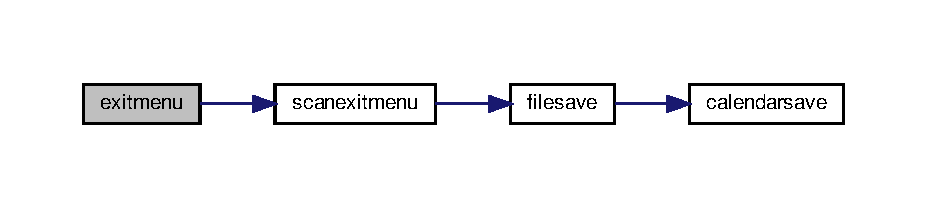
\includegraphics[width=335pt]{menu_8c_ac651d3838f4da7bf6055fa839621e289_cgraph}
\end{center}
\end{figure}
Here is the caller graph for this function\+:
\nopagebreak
\begin{figure}[H]
\begin{center}
\leavevmode
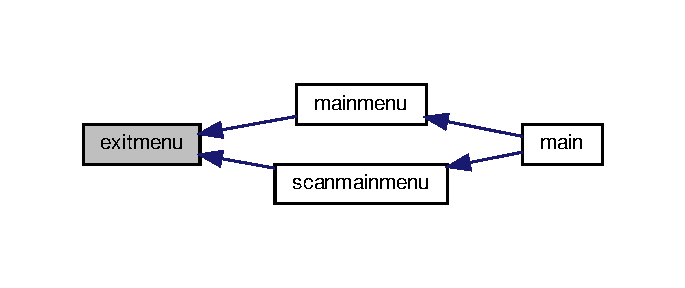
\includegraphics[width=329pt]{menu_8c_ac651d3838f4da7bf6055fa839621e289_icgraph}
\end{center}
\end{figure}
\mbox{\Hypertarget{menu_8c_afc715bc6c0b9a9e85af15dc509a8d34b}\label{menu_8c_afc715bc6c0b9a9e85af15dc509a8d34b}} 
\index{menu.\+c@{menu.\+c}!filesave@{filesave}}
\index{filesave@{filesave}!menu.\+c@{menu.\+c}}
\subsubsection{\texorpdfstring{filesave()}{filesave()}}
{\footnotesize\ttfamily void filesave (\begin{DoxyParamCaption}\item[{\hyperlink{struct_event_list}{Event\+List} $\ast$}]{eventlist }\end{DoxyParamCaption})}

Here is the caller graph for this function\+:
\nopagebreak
\begin{figure}[H]
\begin{center}
\leavevmode
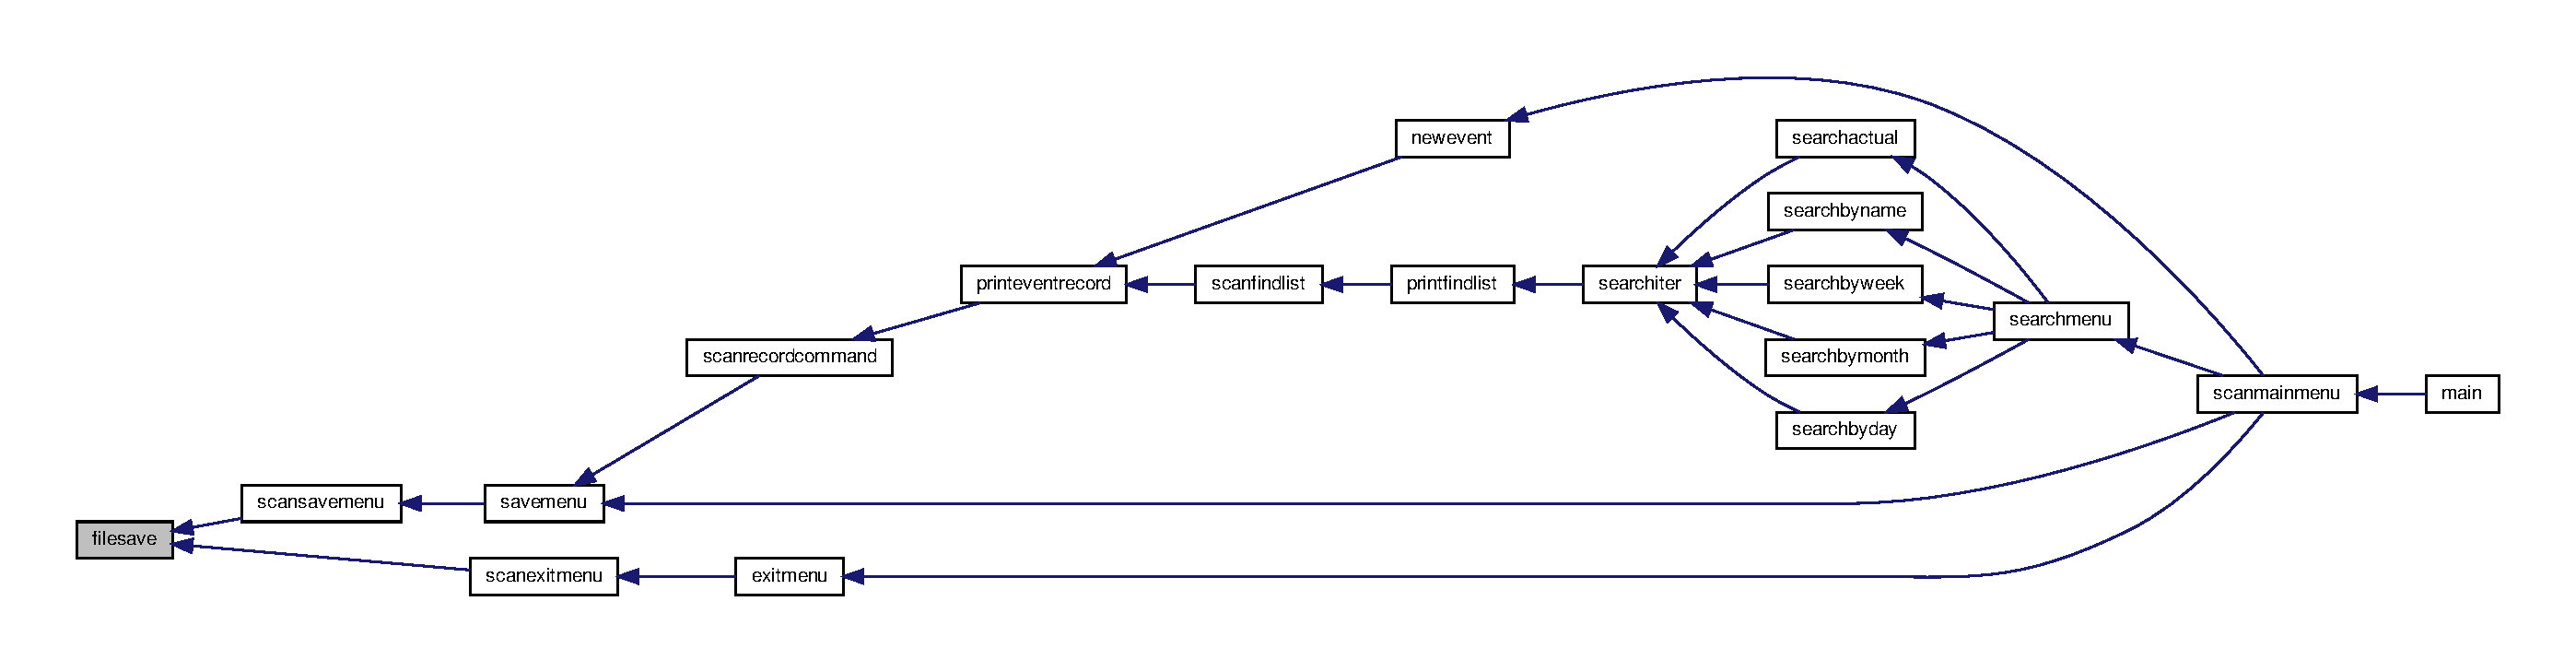
\includegraphics[width=350pt]{menu_8c_afc715bc6c0b9a9e85af15dc509a8d34b_icgraph}
\end{center}
\end{figure}
\mbox{\Hypertarget{menu_8c_ab9ac014b764791c1dc71c187dca898f7}\label{menu_8c_ab9ac014b764791c1dc71c187dca898f7}} 
\index{menu.\+c@{menu.\+c}!hosszu\+\_\+sort\+\_\+olvas@{hosszu\+\_\+sort\+\_\+olvas}}
\index{hosszu\+\_\+sort\+\_\+olvas@{hosszu\+\_\+sort\+\_\+olvas}!menu.\+c@{menu.\+c}}
\subsubsection{\texorpdfstring{hosszu\+\_\+sort\+\_\+olvas()}{hosszu\_sort\_olvas()}}
{\footnotesize\ttfamily char$\ast$ hosszu\+\_\+sort\+\_\+olvas (\begin{DoxyParamCaption}\item[{int}]{bufferhossz }\end{DoxyParamCaption})}

\mbox{\Hypertarget{menu_8c_ac86d3169260f5cacd0f792743957b054}\label{menu_8c_ac86d3169260f5cacd0f792743957b054}} 
\index{menu.\+c@{menu.\+c}!mainmenu@{mainmenu}}
\index{mainmenu@{mainmenu}!menu.\+c@{menu.\+c}}
\subsubsection{\texorpdfstring{mainmenu()}{mainmenu()}}
{\footnotesize\ttfamily void mainmenu (\begin{DoxyParamCaption}{ }\end{DoxyParamCaption})}

Here is the call graph for this function\+:
\nopagebreak
\begin{figure}[H]
\begin{center}
\leavevmode
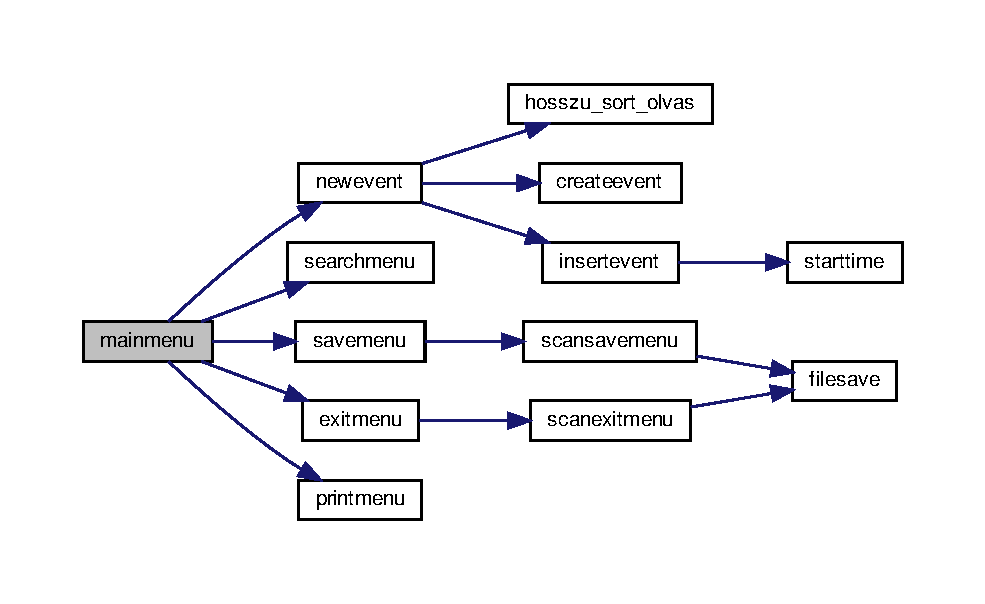
\includegraphics[width=350pt]{menu_8c_ac86d3169260f5cacd0f792743957b054_cgraph}
\end{center}
\end{figure}
Here is the caller graph for this function\+:
\nopagebreak
\begin{figure}[H]
\begin{center}
\leavevmode
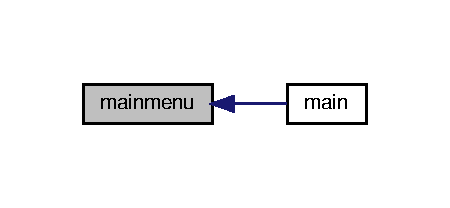
\includegraphics[width=216pt]{menu_8c_ac86d3169260f5cacd0f792743957b054_icgraph}
\end{center}
\end{figure}
\mbox{\Hypertarget{menu_8c_ac2c3136ef241a7150d7cff391a0eb048}\label{menu_8c_ac2c3136ef241a7150d7cff391a0eb048}} 
\index{menu.\+c@{menu.\+c}!newevent@{newevent}}
\index{newevent@{newevent}!menu.\+c@{menu.\+c}}
\subsubsection{\texorpdfstring{newevent()}{newevent()}}
{\footnotesize\ttfamily void newevent (\begin{DoxyParamCaption}\item[{\hyperlink{struct_event_list}{Event\+List} $\ast$}]{eventlist }\end{DoxyParamCaption})}

Here is the call graph for this function\+:
\nopagebreak
\begin{figure}[H]
\begin{center}
\leavevmode
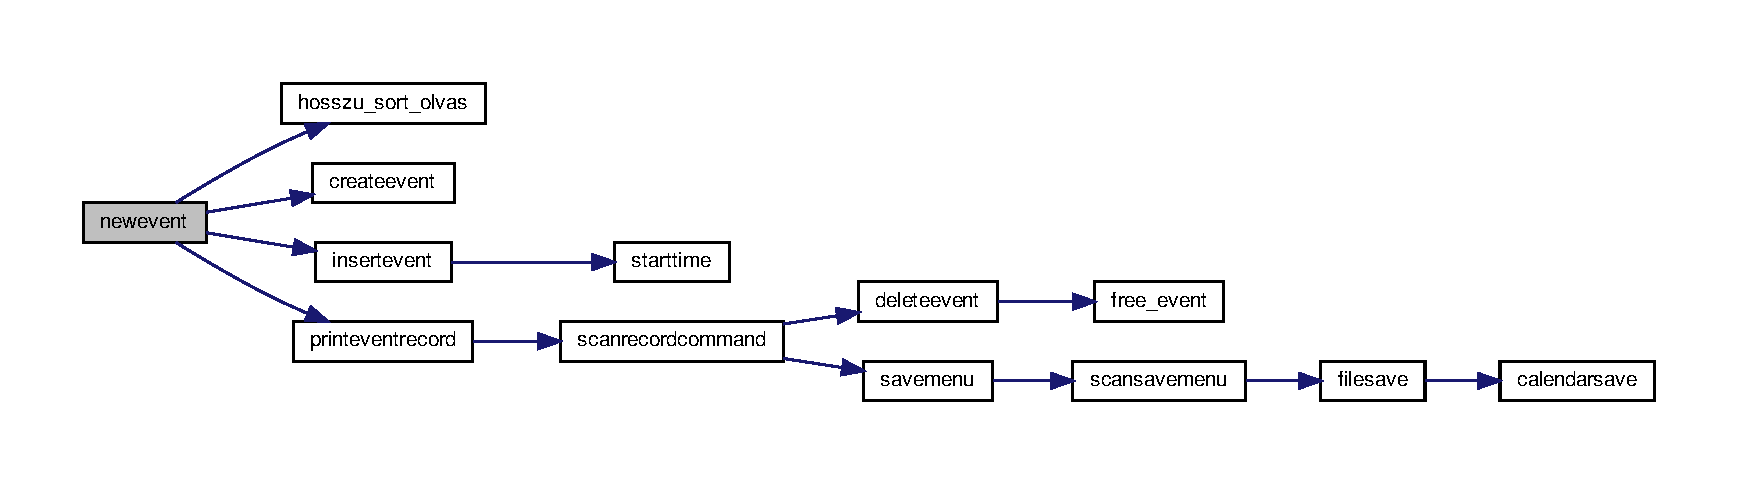
\includegraphics[width=240pt]{menu_8c_ac2c3136ef241a7150d7cff391a0eb048_cgraph}
\end{center}
\end{figure}
Here is the caller graph for this function\+:
\nopagebreak
\begin{figure}[H]
\begin{center}
\leavevmode
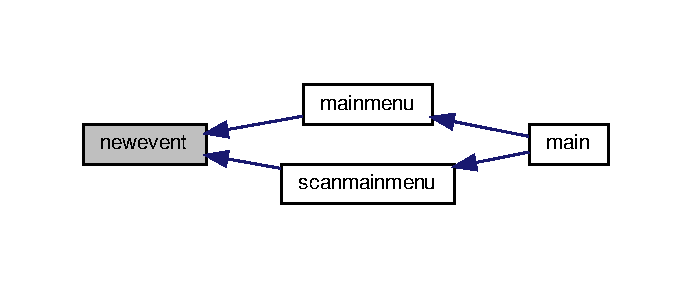
\includegraphics[width=332pt]{menu_8c_ac2c3136ef241a7150d7cff391a0eb048_icgraph}
\end{center}
\end{figure}
\mbox{\Hypertarget{menu_8c_a1aa7ba6b6941a272c34eea491e4a650d}\label{menu_8c_a1aa7ba6b6941a272c34eea491e4a650d}} 
\index{menu.\+c@{menu.\+c}!printmenu@{printmenu}}
\index{printmenu@{printmenu}!menu.\+c@{menu.\+c}}
\subsubsection{\texorpdfstring{printmenu()}{printmenu()}}
{\footnotesize\ttfamily int printmenu (\begin{DoxyParamCaption}\item[{\hyperlink{struct_menu_pont}{Menu\+Pont} $\ast$}]{menupontok }\end{DoxyParamCaption})}

Here is the caller graph for this function\+:
\nopagebreak
\begin{figure}[H]
\begin{center}
\leavevmode
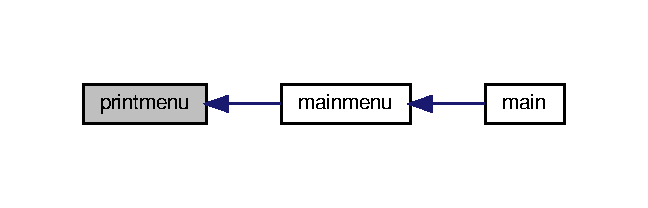
\includegraphics[width=311pt]{menu_8c_a1aa7ba6b6941a272c34eea491e4a650d_icgraph}
\end{center}
\end{figure}
\mbox{\Hypertarget{menu_8c_aa28daf84be098b64b8dfea8a88050f13}\label{menu_8c_aa28daf84be098b64b8dfea8a88050f13}} 
\index{menu.\+c@{menu.\+c}!savemenu@{savemenu}}
\index{savemenu@{savemenu}!menu.\+c@{menu.\+c}}
\subsubsection{\texorpdfstring{savemenu()}{savemenu()}}
{\footnotesize\ttfamily void savemenu (\begin{DoxyParamCaption}\item[{\hyperlink{struct_event_list}{Event\+List} $\ast$}]{eventlist }\end{DoxyParamCaption})}

Here is the call graph for this function\+:
\nopagebreak
\begin{figure}[H]
\begin{center}
\leavevmode
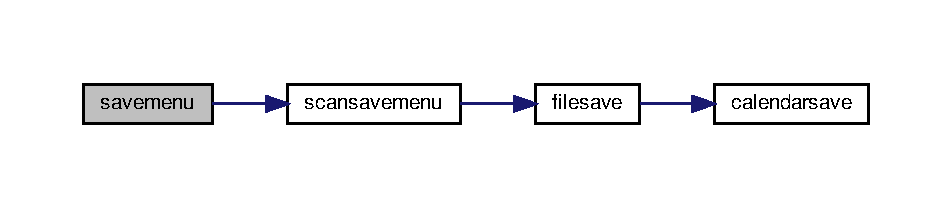
\includegraphics[width=347pt]{menu_8c_aa28daf84be098b64b8dfea8a88050f13_cgraph}
\end{center}
\end{figure}
Here is the caller graph for this function\+:
\nopagebreak
\begin{figure}[H]
\begin{center}
\leavevmode
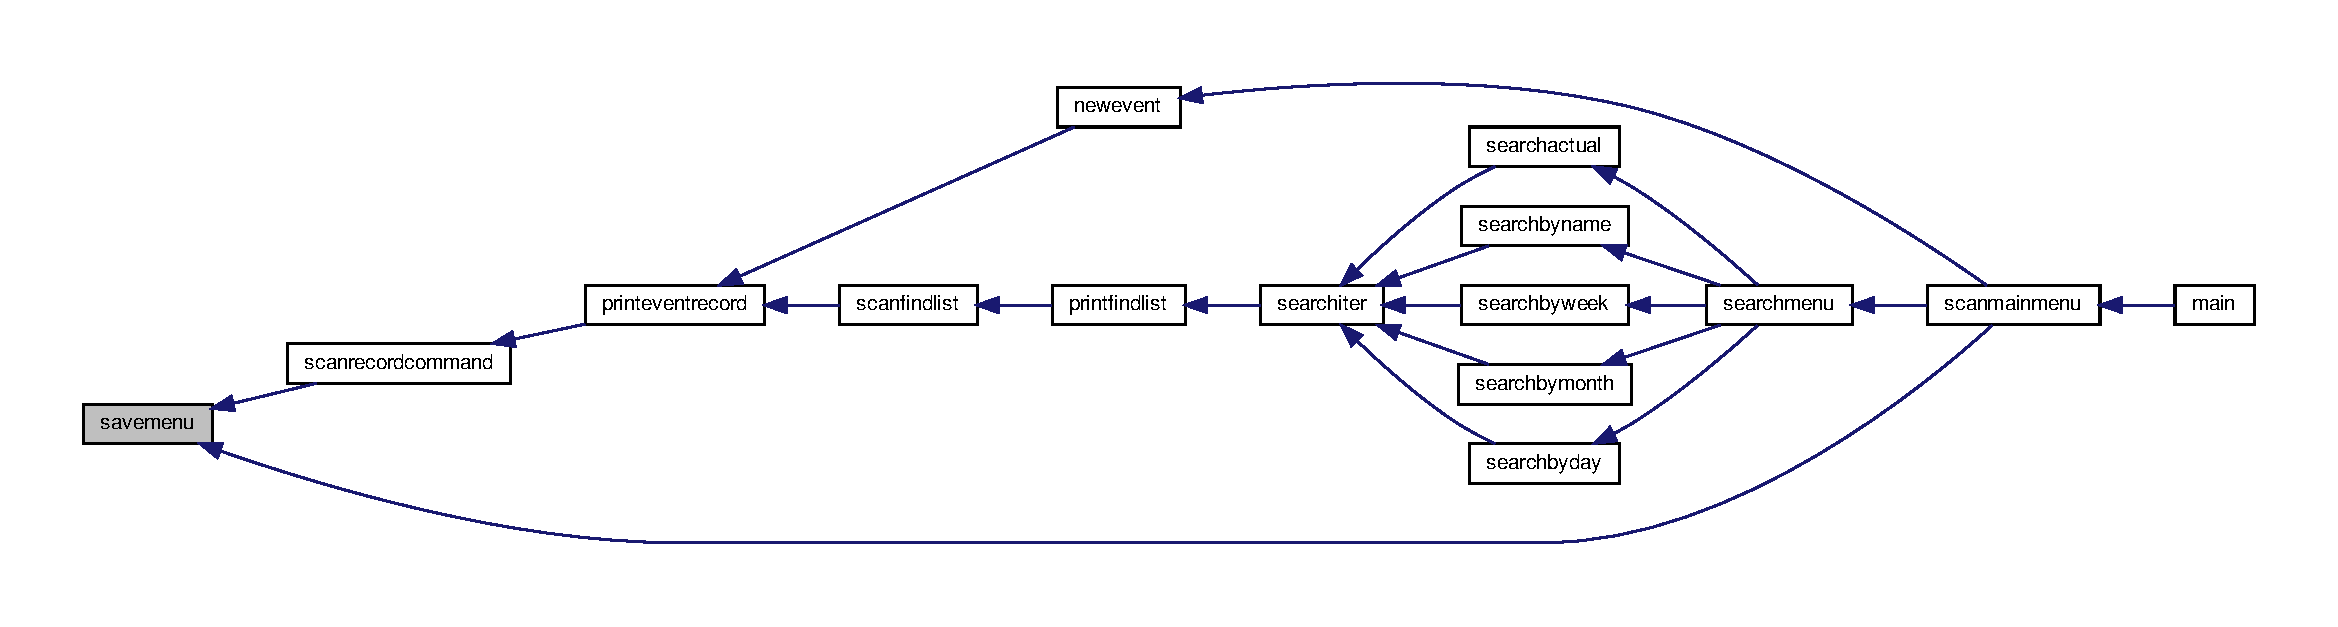
\includegraphics[width=335pt]{menu_8c_aa28daf84be098b64b8dfea8a88050f13_icgraph}
\end{center}
\end{figure}
\mbox{\Hypertarget{menu_8c_aa12eba16d2e2bd5dfc70240d19bd5c8e}\label{menu_8c_aa12eba16d2e2bd5dfc70240d19bd5c8e}} 
\index{menu.\+c@{menu.\+c}!scanexitmenu@{scanexitmenu}}
\index{scanexitmenu@{scanexitmenu}!menu.\+c@{menu.\+c}}
\subsubsection{\texorpdfstring{scanexitmenu()}{scanexitmenu()}}
{\footnotesize\ttfamily int scanexitmenu (\begin{DoxyParamCaption}\item[{\hyperlink{struct_event_list}{Event\+List} $\ast$}]{eventlist }\end{DoxyParamCaption})}

Here is the call graph for this function\+:
\nopagebreak
\begin{figure}[H]
\begin{center}
\leavevmode
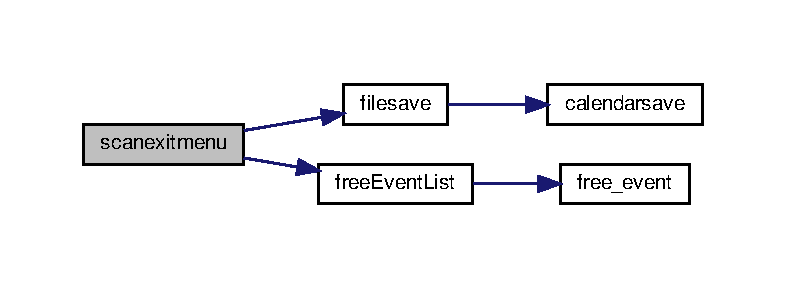
\includegraphics[width=243pt]{menu_8c_aa12eba16d2e2bd5dfc70240d19bd5c8e_cgraph}
\end{center}
\end{figure}
Here is the caller graph for this function\+:
\nopagebreak
\begin{figure}[H]
\begin{center}
\leavevmode
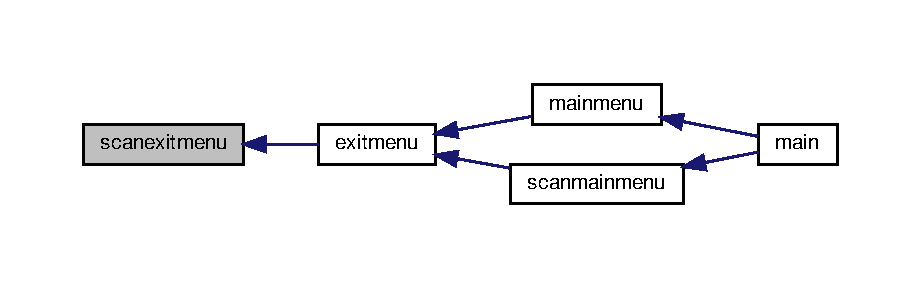
\includegraphics[width=350pt]{menu_8c_aa12eba16d2e2bd5dfc70240d19bd5c8e_icgraph}
\end{center}
\end{figure}
\mbox{\Hypertarget{menu_8c_a8e572ab27981dcd7144340fd25a24c80}\label{menu_8c_a8e572ab27981dcd7144340fd25a24c80}} 
\index{menu.\+c@{menu.\+c}!scanmainmenu@{scanmainmenu}}
\index{scanmainmenu@{scanmainmenu}!menu.\+c@{menu.\+c}}
\subsubsection{\texorpdfstring{scanmainmenu()}{scanmainmenu()}}
{\footnotesize\ttfamily void scanmainmenu (\begin{DoxyParamCaption}\item[{\hyperlink{struct_event_list}{Event\+List} $\ast$}]{eventlist }\end{DoxyParamCaption})}

Here is the call graph for this function\+:
\nopagebreak
\begin{figure}[H]
\begin{center}
\leavevmode
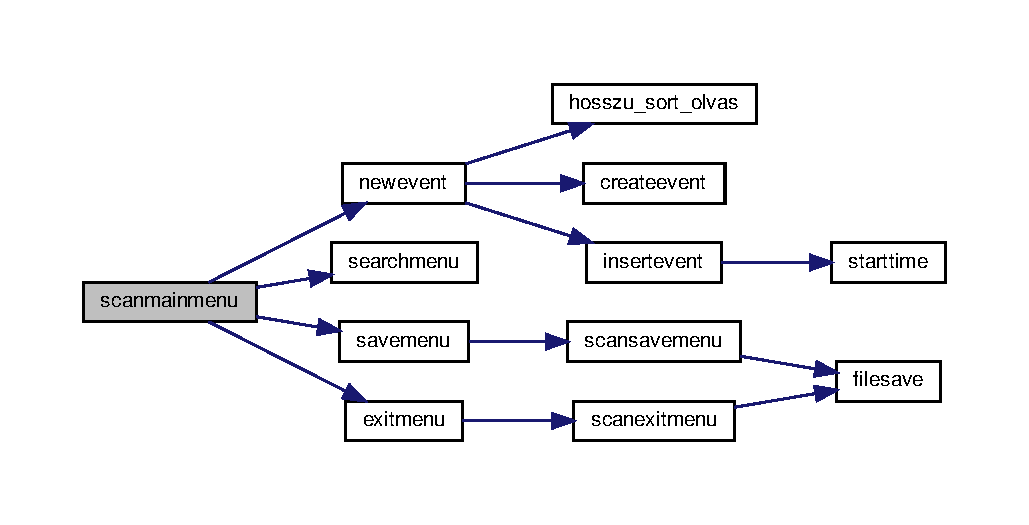
\includegraphics[width=350pt]{menu_8c_a8e572ab27981dcd7144340fd25a24c80_cgraph}
\end{center}
\end{figure}
Here is the caller graph for this function\+:
\nopagebreak
\begin{figure}[H]
\begin{center}
\leavevmode
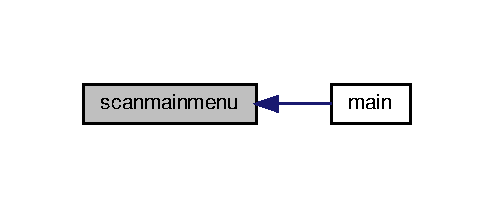
\includegraphics[width=237pt]{menu_8c_a8e572ab27981dcd7144340fd25a24c80_icgraph}
\end{center}
\end{figure}
\mbox{\Hypertarget{menu_8c_a6ef5647864065ede4ef3b2773cbb9e8d}\label{menu_8c_a6ef5647864065ede4ef3b2773cbb9e8d}} 
\index{menu.\+c@{menu.\+c}!scansavemenu@{scansavemenu}}
\index{scansavemenu@{scansavemenu}!menu.\+c@{menu.\+c}}
\subsubsection{\texorpdfstring{scansavemenu()}{scansavemenu()}}
{\footnotesize\ttfamily int scansavemenu (\begin{DoxyParamCaption}\item[{\hyperlink{struct_event_list}{Event\+List} $\ast$}]{eventlist }\end{DoxyParamCaption})}

Here is the call graph for this function\+:
\nopagebreak
\begin{figure}[H]
\begin{center}
\leavevmode
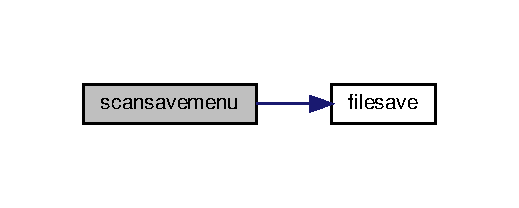
\includegraphics[width=249pt]{menu_8c_a6ef5647864065ede4ef3b2773cbb9e8d_cgraph}
\end{center}
\end{figure}
Here is the caller graph for this function\+:
\nopagebreak
\begin{figure}[H]
\begin{center}
\leavevmode
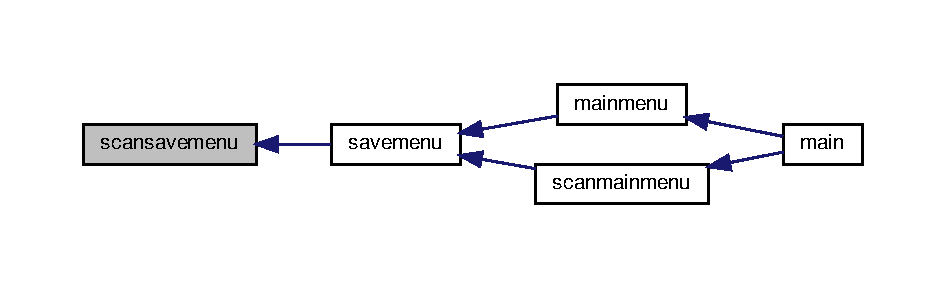
\includegraphics[width=350pt]{menu_8c_a6ef5647864065ede4ef3b2773cbb9e8d_icgraph}
\end{center}
\end{figure}
\mbox{\Hypertarget{menu_8c_a38d64ff02f60ebcb1988655ea12540a6}\label{menu_8c_a38d64ff02f60ebcb1988655ea12540a6}} 
\index{menu.\+c@{menu.\+c}!searchmenu@{searchmenu}}
\index{searchmenu@{searchmenu}!menu.\+c@{menu.\+c}}
\subsubsection{\texorpdfstring{searchmenu()}{searchmenu()}}
{\footnotesize\ttfamily void searchmenu (\begin{DoxyParamCaption}\item[{\hyperlink{struct_event_list}{Event\+List} $\ast$}]{eventlist }\end{DoxyParamCaption})}

Here is the caller graph for this function\+:
\nopagebreak
\begin{figure}[H]
\begin{center}
\leavevmode
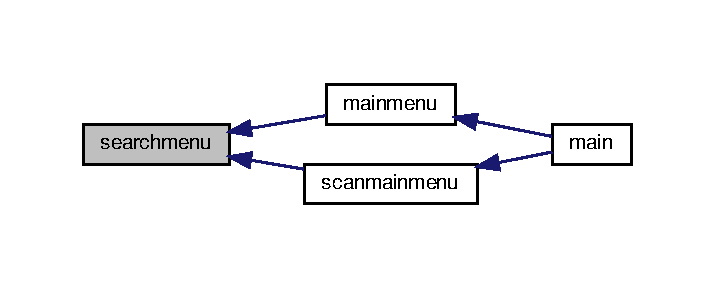
\includegraphics[width=343pt]{menu_8c_a38d64ff02f60ebcb1988655ea12540a6_icgraph}
\end{center}
\end{figure}

\hypertarget{menu_8h}{}\section{/home/dani/\+Documents/egyetem/prog1/nagyhazi/hazi2/calendar2/calendar/menu.h File Reference}
\label{menu_8h}\index{/home/dani/\+Documents/egyetem/prog1/nagyhazi/hazi2/calendar2/calendar/menu.\+h@{/home/dani/\+Documents/egyetem/prog1/nagyhazi/hazi2/calendar2/calendar/menu.\+h}}
{\ttfamily \#include \char`\"{}structures.\+h\char`\"{}}\newline
Include dependency graph for menu.\+h\+:
\nopagebreak
\begin{figure}[H]
\begin{center}
\leavevmode
\includegraphics[width=243pt]{menu_8h__incl}
\end{center}
\end{figure}
This graph shows which files directly or indirectly include this file\+:
\nopagebreak
\begin{figure}[H]
\begin{center}
\leavevmode
\includegraphics[width=350pt]{menu_8h__dep__incl}
\end{center}
\end{figure}
\subsection*{Functions}
\begin{DoxyCompactItemize}
\item 
void \hyperlink{menu_8h_a3fdfc75c2b95c21791f612f12c5a375d}{newevent} ()
\item 
void \hyperlink{menu_8h_a10d0e656ac5ff3a51135fee280274efa}{searchmenu} ()
\item 
void \hyperlink{menu_8h_a928aa131670ac3515aaacdeebb3e278a}{savemenu} ()
\item 
void \hyperlink{menu_8h_ada5bc1a6285c236343ce8a43ac9ab6cc}{exitmenu} ()
\item 
int \hyperlink{menu_8h_a1aa7ba6b6941a272c34eea491e4a650d}{printmenu} (\hyperlink{struct_menu_pont}{Menu\+Pont} $\ast$menupontok)
\item 
char $\ast$ \hyperlink{menu_8h_ab9ac014b764791c1dc71c187dca898f7}{hosszu\+\_\+sort\+\_\+olvas} (int bufferhossz)
\end{DoxyCompactItemize}


\subsection{Function Documentation}
\mbox{\Hypertarget{menu_8h_ada5bc1a6285c236343ce8a43ac9ab6cc}\label{menu_8h_ada5bc1a6285c236343ce8a43ac9ab6cc}} 
\index{menu.\+h@{menu.\+h}!exitmenu@{exitmenu}}
\index{exitmenu@{exitmenu}!menu.\+h@{menu.\+h}}
\subsubsection{\texorpdfstring{exitmenu()}{exitmenu()}}
{\footnotesize\ttfamily void exitmenu (\begin{DoxyParamCaption}{ }\end{DoxyParamCaption})}

\mbox{\Hypertarget{menu_8h_ab9ac014b764791c1dc71c187dca898f7}\label{menu_8h_ab9ac014b764791c1dc71c187dca898f7}} 
\index{menu.\+h@{menu.\+h}!hosszu\+\_\+sort\+\_\+olvas@{hosszu\+\_\+sort\+\_\+olvas}}
\index{hosszu\+\_\+sort\+\_\+olvas@{hosszu\+\_\+sort\+\_\+olvas}!menu.\+h@{menu.\+h}}
\subsubsection{\texorpdfstring{hosszu\+\_\+sort\+\_\+olvas()}{hosszu\_sort\_olvas()}}
{\footnotesize\ttfamily char$\ast$ hosszu\+\_\+sort\+\_\+olvas (\begin{DoxyParamCaption}\item[{int}]{bufferhossz }\end{DoxyParamCaption})}

Here is the caller graph for this function\+:
\nopagebreak
\begin{figure}[H]
\begin{center}
\leavevmode
\includegraphics[width=350pt]{menu_8h_ab9ac014b764791c1dc71c187dca898f7_icgraph}
\end{center}
\end{figure}
\mbox{\Hypertarget{menu_8h_a3fdfc75c2b95c21791f612f12c5a375d}\label{menu_8h_a3fdfc75c2b95c21791f612f12c5a375d}} 
\index{menu.\+h@{menu.\+h}!newevent@{newevent}}
\index{newevent@{newevent}!menu.\+h@{menu.\+h}}
\subsubsection{\texorpdfstring{newevent()}{newevent()}}
{\footnotesize\ttfamily void newevent (\begin{DoxyParamCaption}{ }\end{DoxyParamCaption})}

\mbox{\Hypertarget{menu_8h_a1aa7ba6b6941a272c34eea491e4a650d}\label{menu_8h_a1aa7ba6b6941a272c34eea491e4a650d}} 
\index{menu.\+h@{menu.\+h}!printmenu@{printmenu}}
\index{printmenu@{printmenu}!menu.\+h@{menu.\+h}}
\subsubsection{\texorpdfstring{printmenu()}{printmenu()}}
{\footnotesize\ttfamily int printmenu (\begin{DoxyParamCaption}\item[{\hyperlink{struct_menu_pont}{Menu\+Pont} $\ast$}]{menupontok }\end{DoxyParamCaption})}

Here is the caller graph for this function\+:
\nopagebreak
\begin{figure}[H]
\begin{center}
\leavevmode
\includegraphics[width=311pt]{menu_8h_a1aa7ba6b6941a272c34eea491e4a650d_icgraph}
\end{center}
\end{figure}
\mbox{\Hypertarget{menu_8h_a928aa131670ac3515aaacdeebb3e278a}\label{menu_8h_a928aa131670ac3515aaacdeebb3e278a}} 
\index{menu.\+h@{menu.\+h}!savemenu@{savemenu}}
\index{savemenu@{savemenu}!menu.\+h@{menu.\+h}}
\subsubsection{\texorpdfstring{savemenu()}{savemenu()}}
{\footnotesize\ttfamily void savemenu (\begin{DoxyParamCaption}{ }\end{DoxyParamCaption})}

\mbox{\Hypertarget{menu_8h_a10d0e656ac5ff3a51135fee280274efa}\label{menu_8h_a10d0e656ac5ff3a51135fee280274efa}} 
\index{menu.\+h@{menu.\+h}!searchmenu@{searchmenu}}
\index{searchmenu@{searchmenu}!menu.\+h@{menu.\+h}}
\subsubsection{\texorpdfstring{searchmenu()}{searchmenu()}}
{\footnotesize\ttfamily void searchmenu (\begin{DoxyParamCaption}{ }\end{DoxyParamCaption})}


\hypertarget{search_8c}{}\section{/home/dani/\+Documents/egyetem/prog1/nagyhazi/hazi2/calendar2/calendar/search.c File Reference}
\label{search_8c}\index{/home/dani/\+Documents/egyetem/prog1/nagyhazi/hazi2/calendar2/calendar/search.\+c@{/home/dani/\+Documents/egyetem/prog1/nagyhazi/hazi2/calendar2/calendar/search.\+c}}
{\ttfamily \#include \char`\"{}search.\+h\char`\"{}}\newline
{\ttfamily \#include \char`\"{}structures.\+h\char`\"{}}\newline
{\ttfamily \#include $<$stdlib.\+h$>$}\newline
{\ttfamily \#include $<$string.\+h$>$}\newline
{\ttfamily \#include $<$stdbool.\+h$>$}\newline
{\ttfamily \#include $<$time.\+h$>$}\newline
{\ttfamily \#include $<$stdio.\+h$>$}\newline
{\ttfamily \#include \char`\"{}searchui.\+h\char`\"{}}\newline
\subsection*{Functions}
\begin{DoxyCompactItemize}
\item 
int \hyperlink{group__search_ga199722ea7869f598848648238f88d274}{searchiter} (\hyperlink{struct_event_list}{Event\+List} $\ast$eventlist, \hyperlink{struct_search_conditions}{Search\+Conditions} condition)
\item 
int \hyperlink{group__search_ga9a7e3230097d2f97a58082ff6eb864ac}{searchactual} (\hyperlink{struct_event_list}{Event\+List} $\ast$eventlist, \hyperlink{group__search_gaf9df49b17c9441844cafc15064ec50fc}{Search\+By} searchmode)
\item 
void \hyperlink{group__search_gace601ce27f555e73988b2db946d1ca5e}{inserttofindlist} (\hyperlink{struct_find_list}{Find\+List} $\ast$findlist, \hyperlink{struct_event}{Event} $\ast$event)
\item 
int \hyperlink{group__search_ga4e80bfd47c2fef45e9f6f50632544931}{tmtoweek} (\hyperlink{group__list_gaffc453d30a4a6ce81ed778fd04d2d256}{Tm} $\ast$tm)
\item 
\hyperlink{group__list_gaffc453d30a4a6ce81ed778fd04d2d256}{Tm} $\ast$ \hyperlink{group__search_gaa13cd0a956bc531fe1e1329b6aebdef9}{eventtotm} (\hyperlink{struct_event}{Event} $\ast$event)
\end{DoxyCompactItemize}

\hypertarget{search_8h}{}\section{/home/dani/\+Documents/egyetem/prog1/nagyhazi/hazi2/calendar2/calendar/search.h File Reference}
\label{search_8h}\index{/home/dani/\+Documents/egyetem/prog1/nagyhazi/hazi2/calendar2/calendar/search.\+h@{/home/dani/\+Documents/egyetem/prog1/nagyhazi/hazi2/calendar2/calendar/search.\+h}}
{\ttfamily \#include $<$stdbool.\+h$>$}\newline
{\ttfamily \#include \char`\"{}structures.\+h\char`\"{}}\newline
\subsection*{Typedefs}
\begin{DoxyCompactItemize}
\item 
typedef enum \hyperlink{group__search_gaf9df49b17c9441844cafc15064ec50fc}{Search\+By} \hyperlink{group__search_ga2ab4e565bcf990b57e010007e13bec43}{Search\+By}
\end{DoxyCompactItemize}
\subsection*{Enumerations}
\begin{DoxyCompactItemize}
\item 
enum \hyperlink{group__search_gaf9df49b17c9441844cafc15064ec50fc}{Search\+By} \{ \hyperlink{group__search_ggaf9df49b17c9441844cafc15064ec50fca22234af7e39a964f41baef92fdd17c14}{byweek}, 
\hyperlink{group__search_ggaf9df49b17c9441844cafc15064ec50fca5efad3bcd6c0ae75087b25e99c9483fa}{byday}, 
\hyperlink{group__search_ggaf9df49b17c9441844cafc15064ec50fca1079e56084842bedf75f880e98175b84}{bymonth}
 \}
\end{DoxyCompactItemize}
\subsection*{Functions}
\begin{DoxyCompactItemize}
\item 
int \hyperlink{group__search_ga199722ea7869f598848648238f88d274}{searchiter} (\hyperlink{struct_event_list}{Event\+List} $\ast$eventlist, \hyperlink{struct_search_conditions}{Search\+Conditions} condition)
\item 
int \hyperlink{group__search_ga9a7e3230097d2f97a58082ff6eb864ac}{searchactual} (\hyperlink{struct_event_list}{Event\+List} $\ast$eventlist, \hyperlink{group__search_gaf9df49b17c9441844cafc15064ec50fc}{Search\+By} searchmode)
\item 
void \hyperlink{group__search_gace601ce27f555e73988b2db946d1ca5e}{inserttofindlist} (\hyperlink{struct_find_list}{Find\+List} $\ast$findlist, \hyperlink{struct_event}{Event} $\ast$event)
\item 
int \hyperlink{group__search_ga4e80bfd47c2fef45e9f6f50632544931}{tmtoweek} (\hyperlink{group__list_gaffc453d30a4a6ce81ed778fd04d2d256}{Tm} $\ast$tm)
\item 
\hyperlink{group__list_gaffc453d30a4a6ce81ed778fd04d2d256}{Tm} $\ast$ \hyperlink{group__search_gaa13cd0a956bc531fe1e1329b6aebdef9}{eventtotm} (\hyperlink{struct_event}{Event} $\ast$event)
\end{DoxyCompactItemize}

\hypertarget{searchui_8c}{}\section{/home/dani/\+Documents/egyetem/prog1/nagyhazi/hazi2/calendar2/calendar/searchui.c File Reference}
\label{searchui_8c}\index{/home/dani/\+Documents/egyetem/prog1/nagyhazi/hazi2/calendar2/calendar/searchui.\+c@{/home/dani/\+Documents/egyetem/prog1/nagyhazi/hazi2/calendar2/calendar/searchui.\+c}}
{\ttfamily \#include \char`\"{}structures.\+h\char`\"{}}\newline
{\ttfamily \#include $<$stdbool.\+h$>$}\newline
{\ttfamily \#include $<$stdio.\+h$>$}\newline
\subsection*{Functions}
\begin{DoxyCompactItemize}
\item 
int \hyperlink{group__search_ga0ab78ad9b3d9c7fe1975fd416a1f1c5c}{scaninput} ()
\item 
int \hyperlink{group__search_gadaf3bc7221b1fe4f2cffb3aaea00415d}{searchbyname} (\hyperlink{struct_event_list}{Event\+List} $\ast$eventlist)
\item 
int \hyperlink{group__search_ga6b219250779d3af5972611513010a013}{searchbyweek} (\hyperlink{struct_event_list}{Event\+List} $\ast$eventlist)
\item 
int \hyperlink{group__search_gac2a6873263c1a8146c04126b48f8431e}{searchbymonth} (\hyperlink{struct_event_list}{Event\+List} $\ast$eventlist)
\item 
int \hyperlink{group__search_ga5a5f902f17fae2dda3b8ec6bb7e1a6e9}{searchbyday} (\hyperlink{struct_event_list}{Event\+List} $\ast$eventlist)
\item 
int \hyperlink{group__search_ga4fc3c2695bbc6aacac6fcdddbbc2c9ea}{printfindlist} (\hyperlink{struct_find_list}{Find\+List} $\ast$findlist, \hyperlink{struct_search_conditions}{Search\+Conditions} condition, \hyperlink{struct_event_list}{Event\+List} $\ast$eventlist)
\item 
int \hyperlink{group__search_ga70f4e24bc56ccfdd7d63df4a84054538}{scanfindlist} (int i, \hyperlink{struct_find_list}{Find\+List} $\ast$findlist, \hyperlink{struct_search_conditions}{Search\+Conditions} condition, \hyperlink{struct_event_list}{Event\+List} $\ast$eventlist)
\item 
void \hyperlink{group__search_ga2561d96be1299fd3f5730c6d82143709}{printevent\+\_\+short} (\hyperlink{struct_event}{Event} $\ast$event)
\end{DoxyCompactItemize}

\hypertarget{searchui_8h}{}\section{/home/dani/\+Documents/egyetem/prog1/nagyhazi/hazi2/calendar2/calendar/searchui.h File Reference}
\label{searchui_8h}\index{/home/dani/\+Documents/egyetem/prog1/nagyhazi/hazi2/calendar2/calendar/searchui.\+h@{/home/dani/\+Documents/egyetem/prog1/nagyhazi/hazi2/calendar2/calendar/searchui.\+h}}
\subsection*{Functions}
\begin{DoxyCompactItemize}
\item 
int \hyperlink{group__search_ga0ab78ad9b3d9c7fe1975fd416a1f1c5c}{scaninput} ()
\item 
int \hyperlink{group__search_gadaf3bc7221b1fe4f2cffb3aaea00415d}{searchbyname} (\hyperlink{struct_event_list}{Event\+List} $\ast$eventlist)
\item 
int \hyperlink{group__search_ga6b219250779d3af5972611513010a013}{searchbyweek} (\hyperlink{struct_event_list}{Event\+List} $\ast$eventlist)
\item 
int \hyperlink{group__search_gac2a6873263c1a8146c04126b48f8431e}{searchbymonth} (\hyperlink{struct_event_list}{Event\+List} $\ast$eventlist)
\item 
int \hyperlink{group__search_ga5a5f902f17fae2dda3b8ec6bb7e1a6e9}{searchbyday} (\hyperlink{struct_event_list}{Event\+List} $\ast$eventlist)
\item 
int \hyperlink{group__search_ga4fc3c2695bbc6aacac6fcdddbbc2c9ea}{printfindlist} (\hyperlink{struct_find_list}{Find\+List} $\ast$findlist, \hyperlink{struct_search_conditions}{Search\+Conditions} condition, \hyperlink{struct_event_list}{Event\+List} $\ast$eventlist)
\item 
int \hyperlink{group__search_ga70f4e24bc56ccfdd7d63df4a84054538}{scanfindlist} (int i, \hyperlink{struct_find_list}{Find\+List} $\ast$findlist, \hyperlink{struct_search_conditions}{Search\+Conditions} condition, \hyperlink{struct_event_list}{Event\+List} $\ast$eventlist)
\item 
void \hyperlink{group__search_ga2561d96be1299fd3f5730c6d82143709}{printevent\+\_\+short} (\hyperlink{struct_event}{Event} $\ast$event)
\end{DoxyCompactItemize}

\hypertarget{structures_8h}{}\section{/home/dani/\+Documents/egyetem/prog1/nagyhazi/hazi2/calendar2/calendar/structures.h File Reference}
\label{structures_8h}\index{/home/dani/\+Documents/egyetem/prog1/nagyhazi/hazi2/calendar2/calendar/structures.\+h@{/home/dani/\+Documents/egyetem/prog1/nagyhazi/hazi2/calendar2/calendar/structures.\+h}}
{\ttfamily \#include $<$time.\+h$>$}\newline
Include dependency graph for structures.\+h\+:\nopagebreak
\begin{figure}[H]
\begin{center}
\leavevmode
\includegraphics[width=208pt]{structures_8h__incl}
\end{center}
\end{figure}
This graph shows which files directly or indirectly include this file\+:\nopagebreak
\begin{figure}[H]
\begin{center}
\leavevmode
\includegraphics[width=350pt]{structures_8h__dep__incl}
\end{center}
\end{figure}
\subsection*{Data Structures}
\begin{DoxyCompactItemize}
\item 
struct \hyperlink{struct_event}{Event}
\item 
struct \hyperlink{struct_event_list}{Event\+List}
\item 
struct \hyperlink{struct_found_event}{Found\+Event}
\item 
struct \hyperlink{struct_find_list}{Find\+List}
\item 
struct \hyperlink{struct_search_conditions}{Search\+Conditions}
\item 
struct \hyperlink{struct_menu_pont}{Menu\+Pont}
\end{DoxyCompactItemize}
\subsection*{Typedefs}
\begin{DoxyCompactItemize}
\item 
typedef struct \hyperlink{struct_event}{Event} \hyperlink{structures_8h_a607b119a19e65e2c1c7a606f21ab7a46}{Event}
\item 
typedef struct \hyperlink{struct_event_list}{Event\+List} \hyperlink{structures_8h_a7faf24c32c52b92939a97982baf9dedf}{Event\+List}
\item 
typedef struct \hyperlink{struct_found_event}{Found\+Event} \hyperlink{structures_8h_ac0286403197d5147979a4986c9425222}{Found\+Event}
\item 
typedef struct \hyperlink{struct_find_list}{Find\+List} \hyperlink{structures_8h_ad7aca260cf976ef8a90cbe97ab5dba48}{Find\+List}
\item 
typedef struct \hyperlink{struct_search_conditions}{Search\+Conditions} \hyperlink{structures_8h_adc5706147428e7cb68faa6fb19085d7a}{Search\+Conditions}
\item 
typedef void($\ast$ \hyperlink{structures_8h_aa04041873905737ffeb12c611f7c5bde}{Menu\+Fv}) (\hyperlink{struct_event_list}{Event\+List} $\ast$)
\item 
typedef struct \hyperlink{struct_menu_pont}{Menu\+Pont} \hyperlink{structures_8h_a0ef80ab3e0ae7fe6915f17204e5f6211}{Menu\+Pont}
\item 
typedef struct tm \hyperlink{structures_8h_affc453d30a4a6ce81ed778fd04d2d256}{Tm}
\end{DoxyCompactItemize}


\subsection{Typedef Documentation}
\mbox{\Hypertarget{structures_8h_a607b119a19e65e2c1c7a606f21ab7a46}\label{structures_8h_a607b119a19e65e2c1c7a606f21ab7a46}} 
\index{structures.\+h@{structures.\+h}!Event@{Event}}
\index{Event@{Event}!structures.\+h@{structures.\+h}}
\subsubsection{\texorpdfstring{Event}{Event}}
{\footnotesize\ttfamily typedef struct \hyperlink{struct_event}{Event} \hyperlink{struct_event}{Event}}

\mbox{\Hypertarget{structures_8h_a7faf24c32c52b92939a97982baf9dedf}\label{structures_8h_a7faf24c32c52b92939a97982baf9dedf}} 
\index{structures.\+h@{structures.\+h}!Event\+List@{Event\+List}}
\index{Event\+List@{Event\+List}!structures.\+h@{structures.\+h}}
\subsubsection{\texorpdfstring{Event\+List}{EventList}}
{\footnotesize\ttfamily typedef struct \hyperlink{struct_event_list}{Event\+List} \hyperlink{struct_event_list}{Event\+List}}

\mbox{\Hypertarget{structures_8h_ad7aca260cf976ef8a90cbe97ab5dba48}\label{structures_8h_ad7aca260cf976ef8a90cbe97ab5dba48}} 
\index{structures.\+h@{structures.\+h}!Find\+List@{Find\+List}}
\index{Find\+List@{Find\+List}!structures.\+h@{structures.\+h}}
\subsubsection{\texorpdfstring{Find\+List}{FindList}}
{\footnotesize\ttfamily typedef struct \hyperlink{struct_find_list}{Find\+List} \hyperlink{struct_find_list}{Find\+List}}

\mbox{\Hypertarget{structures_8h_ac0286403197d5147979a4986c9425222}\label{structures_8h_ac0286403197d5147979a4986c9425222}} 
\index{structures.\+h@{structures.\+h}!Found\+Event@{Found\+Event}}
\index{Found\+Event@{Found\+Event}!structures.\+h@{structures.\+h}}
\subsubsection{\texorpdfstring{Found\+Event}{FoundEvent}}
{\footnotesize\ttfamily typedef struct \hyperlink{struct_found_event}{Found\+Event} \hyperlink{struct_found_event}{Found\+Event}}

\mbox{\Hypertarget{structures_8h_aa04041873905737ffeb12c611f7c5bde}\label{structures_8h_aa04041873905737ffeb12c611f7c5bde}} 
\index{structures.\+h@{structures.\+h}!Menu\+Fv@{Menu\+Fv}}
\index{Menu\+Fv@{Menu\+Fv}!structures.\+h@{structures.\+h}}
\subsubsection{\texorpdfstring{Menu\+Fv}{MenuFv}}
{\footnotesize\ttfamily typedef void($\ast$ Menu\+Fv) (\hyperlink{struct_event_list}{Event\+List} $\ast$)}

\mbox{\Hypertarget{structures_8h_a0ef80ab3e0ae7fe6915f17204e5f6211}\label{structures_8h_a0ef80ab3e0ae7fe6915f17204e5f6211}} 
\index{structures.\+h@{structures.\+h}!Menu\+Pont@{Menu\+Pont}}
\index{Menu\+Pont@{Menu\+Pont}!structures.\+h@{structures.\+h}}
\subsubsection{\texorpdfstring{Menu\+Pont}{MenuPont}}
{\footnotesize\ttfamily typedef struct \hyperlink{struct_menu_pont}{Menu\+Pont}  \hyperlink{struct_menu_pont}{Menu\+Pont}}

\mbox{\Hypertarget{structures_8h_adc5706147428e7cb68faa6fb19085d7a}\label{structures_8h_adc5706147428e7cb68faa6fb19085d7a}} 
\index{structures.\+h@{structures.\+h}!Search\+Conditions@{Search\+Conditions}}
\index{Search\+Conditions@{Search\+Conditions}!structures.\+h@{structures.\+h}}
\subsubsection{\texorpdfstring{Search\+Conditions}{SearchConditions}}
{\footnotesize\ttfamily typedef struct \hyperlink{struct_search_conditions}{Search\+Conditions} \hyperlink{struct_search_conditions}{Search\+Conditions}}

\mbox{\Hypertarget{structures_8h_affc453d30a4a6ce81ed778fd04d2d256}\label{structures_8h_affc453d30a4a6ce81ed778fd04d2d256}} 
\index{structures.\+h@{structures.\+h}!Tm@{Tm}}
\index{Tm@{Tm}!structures.\+h@{structures.\+h}}
\subsubsection{\texorpdfstring{Tm}{Tm}}
{\footnotesize\ttfamily typedef struct tm \hyperlink{list_8h_affc453d30a4a6ce81ed778fd04d2d256}{Tm}}


%--- End generated contents ---

% Index
\backmatter
\newpage
\phantomsection
\clearemptydoublepage
\addcontentsline{toc}{chapter}{Index}
\printindex

\end{document}
